\documentclass[12pt, a4paper, reqno, oneside]{book}
\usepackage[left=2.5cm, right=2cm, top=2cm, bottom=2cm]{geometry}
\usepackage{amsmath,amsxtra,amssymb,latexsym, amscd,amsthm}
\usepackage{microtype}
\usepackage{indentfirst}
\usepackage{color}
\usepackage{empheq}
\usepackage{iftex}
\ifXeTeX
  \usepackage{fontspec}
  \setmainfont[Ligatures=TeX]{Times New Roman}
  \setsansfont[Ligatures=TeX]{Arial}
  \usepackage[english,vietnamese]{babel}
\else
  \usepackage[utf8]{inputenc}
  \usepackage[T5,T1]{fontenc}
  \usepackage[vietnamese,USenglish]{babel}
\fi
% \usepackage{amsmath} % already loaded on line 3
\usepackage[mathscr]{eucal}
\usepackage{amsfonts}
\usepackage{graphicx}
\usepackage{float}
\usepackage{listings}
\usepackage[dvipsnames]{xcolor}
\usepackage{verbatim}
\usepackage{tikz}
\usetikzlibrary{calc,positioning,arrows.meta,shapes.geometric,fit,backgrounds,decorations.pathreplacing}
\usepackage{tkz-graph}
\usepackage{array}
\usepackage{multirow}
\usepackage{algorithm}
\usepackage{algpseudocode}
% Note: subfigure is legacy and conflicts with modern subcaption; kept commented for compatibility
% \usepackage{subfigure}
\usepackage{pgfplots}
\pgfplotsset{compat=1.18}
\usepackage{titlesec}
\usepackage{fancyhdr}
\usepackage{rotating}
\usepackage{longtable}
\usepackage{supertabular}
\usepackage{subcaption}
\usepackage{tabularx}
\usepackage[normalem]{ulem}
\usepackage{pdfpages}
\usepackage[square,numbers]{natbib}
\usepackage{booktabs}
\usepackage{chngcntr}
\usepackage{tabularray}
\usepackage{placeins}
\usepackage{enumitem}
\usepackage{seqsplit}
\usepackage{needspace}
\usepackage[labelfont=bf, textfont=it, justification=centering]{caption}
\captionsetup{labelfont={color=blue, bf}, textfont={color=black, it}}
\captionsetup[table]{position=top}
\captionsetup[figure]{position=bottom}

\hyphenation{op-tical net-works semi-conduc-tor}
\usepackage[hyphens,spaces,obeyspaces]{url}
\usepackage{xurl}
\usepackage[colorlinks=true,bookmarksopen,bookmarksnumbered,citecolor=blue,linkcolor=blue,urlcolor=blue,pdftitle={Structural Representation for Cross-Vehicle CAN Bus Intrusion Detection},pdfauthor={Vu Tien Tuan Trung}]{hyperref}
\def\UrlBreaks{\do\/\do-\do_\do.\do=\do?\do&\do~}
\def\UrlNoBreaks{\do\(\do\[\do\{\do\<\do\:}
\setlength{\emergencystretch}{1.5em}

\renewcommand{\baselinestretch}{1.25}
\setlength{\headheight}{15pt}
\setlength{\textfloatsep}{10pt plus 2pt minus 2pt}
\setlength{\intextsep}{8pt plus 2pt minus 2pt}
\setlength{\floatsep}{8pt plus 2pt minus 2pt}
\setlength{\abovecaptionskip}{4pt}
\setlength{\belowcaptionskip}{4pt}
\titleformat{\section}{\normalfont\Large\bfseries\raggedright}{\thesection}{1em}{}
\titleformat{\subsection}{\normalfont\large\bfseries\raggedright}{\thesubsection}{1em}{}
\titleformat{\subsubsection}{\normalfont\normalsize\bfseries\raggedright}{\thesubsubsection}{1em}{}

\fancyhf{}
\fancyhead[L]{\small{\leftmark}}
\fancyfoot[C]{\thepage}

\newcommand\chap[1]{%
  \clearpage\phantomsection%
  \chapter*{#1}%
  \addcontentsline{toc}{chapter}{#1}%
  \markboth{#1}{}%
}
\newcommand\sect[1]{%
  \Needspace{5\baselineskip}%
  \phantomsection%
  \addcontentsline{toc}{section}{#1}%
  \section*{#1}%
}

\renewcommand{\theequation}{\thechapter.\arabic{equation}}
\counterwithin{algorithm}{chapter}
\renewcommand{\thealgorithm}{\thechapter.\arabic{algorithm}}
\floatname{algorithm}{Algorithm}
\renewcommand{\listalgorithmname}{List of Algorithms}
\algrenewcommand\algorithmicrequire{\textbf{Input:}}
\algrenewcommand\algorithmicensure{\textbf{Output:}}
\newtheorem{lemma}{\bf Lemma}[chapter]
\newtheorem{theorem}{\bf Theorem}[chapter]
\newtheorem{proposition}{\bf Proposition}[chapter]
\newtheorem{corollary}{\bf Corollary}[chapter]
\newtheorem{definition}{\bf Definition}[chapter]
\newtheorem{remark}{\bf Remark}[section]

% Mức tiêu đề sâu (subsubsubsection, paragraph)
\titleclass{\subsubsubsection}{straight}[\subsection]
\newcounter{subsubsubsection}[subsubsection]
\renewcommand\thesubsubsubsection{\thesubsubsection.\arabic{subsubsubsection}}
\renewcommand\theparagraph{\thesubsubsubsection.\arabic{paragraph}}

\titleformat{\subsubsubsection}
  {\normalfont\normalsize\bfseries}{\thesubsubsubsection}{1em}{}
\titlespacing*{\subsubsubsection}
  {0pt}{3.25ex plus 1ex minus .2ex}{1.5ex plus .2ex}

\makeatletter
\renewcommand\paragraph{\@startsection{paragraph}{5}{\z@}%
  {3.25ex \@plus1ex \@minus.2ex}%
  {-1em}%
  {\normalfont\normalsize\bfseries}}
\renewcommand\subparagraph{\@startsection{subparagraph}{6}{\parindent}%
  {3.25ex \@plus1ex \@minus .2ex}%
  {-1em}%
  {\normalfont\normalsize\bfseries}}
\def\toclevel@subsubsubsection{4}
\def\toclevel@paragraph{5}
\def\toclevel@paragraph{6}
\def\l@subsubsubsection{\@dottedtocline{4}{7em}{4em}}
\def\l@paragraph{\@dottedtocline{5}{10em}{5em}}
\def\l@subparagraph{\@dottedtocline{6}{14em}{6em}}
\makeatother

\setcounter{secnumdepth}{4}
\setcounter{tocdepth}{2}

% Thư mục hình ảnh
\graphicspath{{./figs/}}

\definecolor{mygreen}{rgb}{0,0.6,0}
\definecolor{mygray}{rgb}{0.5,0.5,0.5}
\definecolor{mymauve}{rgb}{0.58,0,0.82}

\lstdefinestyle{customc}{
  belowcaptionskip=1\baselineskip,
  breaklines=true,
  frame=single,
  xleftmargin=\parindent,
  language=C,
  showstringspaces=false,
  basicstyle=\footnotesize\ttfamily,
  keywordstyle=\bfseries\color{green!40!black},
  commentstyle=\itshape\color{purple!40!black},
  identifierstyle=\color{blue},
  stringstyle=\color{orange},
  numbers=left,
  numberstyle=\tiny\color{gray},
  stepnumber=1, 
}

\lstdefinestyle{customasm}{
  belowcaptionskip=1\baselineskip,
  frame=single,
  xleftmargin=\parindent,
  language=[x86masm]Assembler,
  basicstyle=\footnotesize\ttfamily,
  commentstyle=\itshape\color{purple!40!black},
  numbers=left,
  numberstyle=\tiny\color{gray},
  stepnumber=1, 
}

\lstset{escapechar=@,style=customc}

\definecolor{processblue}{cmyk}{0.96,0,0,0}
\newcolumntype{C}[1]{>{\centering\arraybackslash}p{#1}}
\definecolor{eclipseStrings}{RGB}{42,0.0,255}
\definecolor{eclipseKeywords}{RGB}{127,0,85}
\colorlet{numb}{magenta!60!black}

\lstdefinelanguage{json}{
    basicstyle=\normalfont\ttfamily,
    commentstyle=\color{eclipseStrings},
    stringstyle=\color{eclipseKeywords},
    numbers=left,
    numberstyle=\scriptsize,
    stepnumber=1,
    numbersep=8pt,
    showstringspaces=false,
    breaklines=true,
    frame=lines,
    string=[s]{"}{"},
    comment=[l]{:\ "},
    morecomment=[l]{:"},
    literate=
        *{0}{{{\color{numb}0}}}{1}
         {1}{{{\color{numb}1}}}{1}
         {2}{{{\color{numb}2}}}{1}
         {3}{{{\color{numb}3}}}{1}
         {4}{{{\color{numb}4}}}{1}
         {5}{{{\color{numb}5}}}{1}
         {6}{{{\color{numb}6}}}{1}
         {7}{{{\color{numb}7}}}{1}
         {8}{{{\color{numb}8}}}{1}
         {9}{{{\color{numb}9}}}{1}
}

\DeclareRobustCommand{\code}[1]{\nolinkurl{#1}}
\newcolumntype{Y}{>{\raggedright\arraybackslash}X}
\newcolumntype{P}[1]{>{\raggedright\arraybackslash}p{#1}}

\begin{document}
\hypersetup{pageanchor=false}
\selectlanguage{english}

% =========================================================================
% TRANG BÌA NGOÀI (BÌA CHÍNH - KHUNG ĐÔI TIKZ)
% =========================================================================
\begin{titlepage}
\begin{center}
	\begin{tikzpicture}[overlay,remember picture]
	    \draw [line width=3pt,rounded corners=0pt]
	        ($ (current page.north west) + (20mm,-20mm) $)
	        rectangle
	        ($ (current page.south east) + (-15mm,20mm) $);
	    \draw [line width=1pt,rounded corners=0pt]
	        ($ (current page.north west) + (21.5mm,-21.5mm) $)
	        rectangle
	        ($ (current page.south east) + (-16.5mm,21.5mm) $);
	\end{tikzpicture}
	\\[1mm]
    \centerline{\bf VIETNAM NATIONAL UNIVERSITY HANOI}
    \centerline{\bf UNIVERSITY OF ENGINEERING AND TECHNOLOGY}
    
    \vspace*{1.8cm}
    \large
        \begin{figure}[H]
        \centering
        
\includegraphics[width=0.23\linewidth]{figs/uet.jpg}
        \end{figure}
    \vspace*{1cm}
    \centerline{\bf VU TIEN TUAN TRUNG}
    \vspace*{2.0cm}
    {\fontsize{15}{19}\selectfont\bfseries
    \centerline{Structural Representation for}
    \centerline{Cross-Vehicle CAN Bus}
    \centerline{Intrusion Detection\par}}
    \vspace*{2.2cm}
    \centerline{\bf GRADUATION THESIS}
    \vspace*{0.2cm}
    \centerline{\bf Major: Information Systems}
    
    \vfill
    \centerline{\bf Hanoi - 2026}
    \vspace{13pt}
\end{center}
\end{titlepage}

\newpage

% =========================================================================
% TRANG BÌA PHỤ (BÌA TRONG - CÓ CÁN BỘ HƯỚNG DẪN)
% =========================================================================
\begin{titlepage}
\begin{center}
	\begin{tikzpicture}[overlay,remember picture]
	    \draw [line width=3pt,rounded corners=0pt]
	        ($ (current page.north west) + (20mm,-20mm) $)
	        rectangle
	        ($ (current page.south east) + (-15mm,20mm) $);
	    \draw [line width=1pt,rounded corners=0pt]
	        ($ (current page.north west) + (21.5mm,-21.5mm) $)
	        rectangle
	        ($ (current page.south east) + (-16.5mm,21.5mm) $);
	\end{tikzpicture}
	\\[1mm]
    \centerline{\bf VIETNAM NATIONAL UNIVERSITY HANOI}
    \centerline{\bf UNIVERSITY OF ENGINEERING AND TECHNOLOGY}
    \vspace*{1.8cm}
    \large
        \begin{figure}[H]
        \centering
        
\includegraphics[width=0.23\linewidth]{figs/uet.jpg}
        \end{figure}
    \vspace*{0.9cm}
    \large
    \centerline{\bf VU TIEN TUAN TRUNG}
    \vspace*{1.8cm}
    {\fontsize{15}{19}\selectfont\bfseries
    \centerline{Structural Representation for}
    \centerline{Cross-Vehicle CAN Bus}
    \centerline{Intrusion Detection\par}}
    \vspace*{1.5cm}
    \centerline{\bf GRADUATION THESIS}
    \vspace*{0.2cm}
    \centerline{\bf Major: Information Systems}
    
    \vspace*{1.4cm}
    \centerline{\bf Supervisor:}
    \centerline{\bf Assoc. Prof. Nguyen Ngoc Hoa}
    
    \vfill
    \centerline{\bf Hanoi - 2026}
    \vspace{13pt}
\end{center}
\end{titlepage}

\newpage
\hypersetup{pageanchor=true}
\pagenumbering{roman}
\pagestyle{plain}

% =========================================================================
% ACKNOWLEDGEMENTS
% =========================================================================
\chap{Acknowledgements}
\vspace{20pt}
I would like to express my deepest gratitude to my supervisor, Associate Professor Nguyen Ngoc Hoa, for his invaluable guidance, unwavering support, and continuous encouragement throughout this research. His profound expertise, meticulous feedback, and visionary mentorship were instrumental in navigating the complexities of this study, making the completion of this thesis possible.

I also thank the researchers who released open CAN security datasets and publications that enable experimental verification.

During the preparation of this thesis, AI-assisted tools were used for grammar checking, document formatting, literature cross-checking, and programming syntax suggestions. The author personally verified all cited sources, audited and validated the entire codebase, independently conducted all experiments, and assumes full responsibility for the final scientific content; all core ideas, methodological designs, analyses, and conclusions in this thesis constitute the author's independent research work.

While I have strived for academic rigor, I acknowledge that this research still holds potential for further refinement. I warmly welcome and deeply appreciate any constructive critiques and insights from the examination committee, which will undoubtedly help enhance the quality of this work and guide my future endeavors.

Sincere gratitude!

\newpage

% =========================================================================
% AUTHORSHIP DECLARATION
% =========================================================================
\chap{Authorship}
\vspace{20pt}
I declare that this thesis is my original work, conducted under the dedicated supervision of Associate Professor Nguyen Ngoc Hoa. I confirm that this document has not been submitted, either in whole or in part, for any other academic degree or professional qualification at this or any other institution.

All sources, references, and related literature utilized in this study have been comprehensively acknowledged and properly cited. Furthermore, I guarantee that the empirical data and statistical analyses presented herein are the direct results of authentic, independently conducted experiments, ensuring strict methodological rigor and accuracy.

I affirm that this declaration is made with the utmost academic integrity and in full compliance with the academic regulations and policies of the VNU University of Engineering and Technology.

\begin{flushright}
{\it Author}
\hskip 1.5cm\quad

\vskip 2cm
{\bf Vu Tien Tuan Trung}  \quad\ \quad
\end{flushright}

\newpage

% =========================================================================
% ABSTRACT (ENGLISH)
% =========================================================================
\chap{Abstract}
\vspace{15pt}

Cross-vehicle intrusion detection on Controller Area Network (CAN) buses poses a fundamental challenge because message identifiers (CAN-IDs) are manufacturer-proprietary, causing models trained on one vehicle to degrade significantly on unseen platforms. This thesis investigates a 30-dimensional Structural Representation pipeline designed for cross-vehicle intrusion detection, aiming to enable a model trained once in the laboratory to protect diverse vehicle platforms without requiring labeled attack data for retraining on each target vehicle. By excluding raw identifier bits from classifier inputs, the proposed representation captures intrinsic traffic regularities, including intra-window message frequencies, arrival order, sequential transitions, and same-ID payload differences ($\Delta$payload).

Evaluated across four cross-vehicle benchmark sets over three random seeds, empirical results show that under static decision thresholds frozen from source data, structural representations do not automatically boost detection sensitivity (Condition B recall reaches 73.83\% versus 85.41\% for Raw baselines) while target false alarm rates remain elevated ($\text{FAR} = 52.46\%$). However, in threshold-independent ranking, structural features demonstrate clear superiority, increasing Average Precision (AP) from 0.3781 to 0.5554 (+17.74 percentage points paired difference; +17.73 percentage points difference of means over Raw). Phased diagnostic probing reveals that message syntax features inherently retain manufacturer identity (vehicle probe accuracy of 94.88\%) due to feature entanglement between vehicle topology and attack signatures.

To resolve inter-vehicle threshold shift without model retraining, the thesis incorporates an unsupervised benign warmup calibration during initial vehicle ignition ($K = 500$ windows, $\approx 16$ seconds). This lightweight calibration successfully restores operational viability, boosting Condition B recall to 40.42\%--48.59\% while strictly constraining empirical target FAR below 1.08\%, eliminating false-alarm collapse on CICIoV2024, and suppressing Opel Astra DoS false alarms from 31.5\% to 0.17\%.

These findings provide crucial empirical evidence delineating feature ranking quality from operational threshold selection, establishing a reproducible foundation for deployable cross-vehicle automotive intrusion detection systems.

\vspace{1em}
\noindent \textit{\textbf{Keywords:}} CAN bus, intrusion detection, cross-vehicle transfer, structural representation, benign warmup calibration, automotive cybersecurity.

\newpage

% =========================================================================
% DANH MỤC (TOC, LOF, LOT, ABBREVIATIONS)
% =========================================================================
\begingroup
\small
\renewcommand{\baselinestretch}{0.95}\selectfont
\setlength{\parskip}{0pt}
\makeatletter
\renewcommand*\l@chapter[2]{%
  \ifnum \c@tocdepth >\m@ne
    \addpenalty{-\@highpenalty}%
    \vskip 0.25em \@plus\p@
    \setlength\@tempdima{1.5em}%
    \begingroup
      \parindent \z@ \rightskip \@pnumwidth
      \parfillskip -\@pnumwidth
      \leavevmode \bfseries
      \advance\leftskip\@tempdima
      \hskip -\leftskip
      #1\nobreak\hfil \nobreak\hb@xt@\@pnumwidth{\hss #2}\par
      \penalty\@highpenalty
    \endgroup
  \fi}
\makeatother
\tableofcontents
\endgroup
\clearpage

\clearpage
\begingroup
\small
\setlength{\parskip}{0pt}
\phantomsection
\addcontentsline{toc}{chapter}{List of Figures}
\listoffigures
\endgroup
\clearpage

\begingroup
\small
\setlength{\parskip}{0pt}
\phantomsection
\addcontentsline{toc}{chapter}{List of Tables}
\listoftables
\endgroup
\clearpage

\begingroup
\small
\setlength{\parskip}{0pt}
\phantomsection
\addcontentsline{toc}{chapter}{List of Algorithms}
\listofalgorithms
\endgroup
\clearpage

\chap{List of Abbreviations}
\vspace{10pt}
{\small\setlength{\tabcolsep}{4pt}
\noindent\begin{tabularx}{\textwidth}{@{}lYlY@{}}
\toprule
\textbf{Abbreviation} & \textbf{Full Description} & \textbf{Abbreviation} & \textbf{Full Description} \\ \midrule
ACK & Acknowledgment (CAN frame slot) & INLP & Iterative Nullspace Projection \\
AP & Average Precision & LEACE & Least-Squares Concept Erasure \\
CAN & Controller Area Network & LOVO & Leave-One-Vehicle-Out \\
CAN-FD & CAN with Flexible Data-Rate & LR & Logistic Regression \\
CI & Confidence Interval & LRU & Least Recently Used \\
CRC & Cyclic Redundancy Check & LSTM & Long Short-Term Memory \\
CSMA/CD+AMP & Carrier Sense Multiple Access / Collision Detection + Arbitration on Message Priority & MLM & Masked Language Modeling \\
CTT & can-train-and-test dataset & MLP & Multi-Layer Perceptron \\
DANN & Domain-Adversarial Neural Network & OBD-II & On-Board Diagnostics II \\
DBC & CAN Database & PCA & Principal Component Analysis \\
DLC & Data Length Code & PR & Precision--Recall \\
DNN & Deep Neural Network & PR-AUC & Area Under the Precision--Recall Curve \\
DoS & Denial of Service attack & ROC-AUC & Area Under the ROC Curve \\
ECU & Electronic Control Unit & RTR & Remote Transmission Request \\
EOF & End of Frame (CAN frame termination) & SHA-256 & Secure Hash Algorithm 256-bit \\
F1 & Harmonic mean of Precision and Recall & SOF & Start of Frame (CAN frame initiation) \\
FAR & False Alarm Rate (/100k or \%) & TF & Transformer \\
FN/FP & False Negative / False Positive & TF-IDF & Term Frequency--Inv. Doc. Freq. \\
FPR & False Positive Rate & TN/TP & True Negative / True Positive \\
GRL & Gradient Reversal Layer & UET & University of Eng. \& Tech. \\
IDS & Intrusion Detection System & VNU & Vietnam National University \\
\bottomrule
\end{tabularx}\par}
\addtocounter{table}{-1}

\newpage
\pagenumbering{arabic}
\pagestyle{fancy}



\chap{Introduction}\label{chap:introduction}
\sect{Research motivation}
CAN connects electronic control units within a vehicle. The protocol prioritizes communication and bus arbitration but does not provide built-in cryptographic authentication for each sender. Automotive security experiments demonstrate that an attacker with suitable access can influence messages and control functions~\cite{koscher2010experimental,checkoway2011comprehensive}. A passive IDS can monitor traffic without modifying every ECU, but its detection quality must be measured under meaningful deployment conditions.

IDS performance can vary substantially across datasets and evaluation settings~\cite{koltai2026trust}. A model trained on a source vehicle may exploit correlations between attack labels and that vehicle's identifiers, payloads or transmission periods; these correlations may change on a target vehicle. Degradation alone, however, does not prove ID memorization: decision thresholds, sampling, label policies and attack mechanisms may also contribute. This study therefore separates measured performance from hypotheses about its causes.

This thesis uses \texttt{can-train-and-test} as its primary benchmark because the dataset explicitly organizes four evaluation conditions combining known/unseen vehicles and attacks~\cite{lampe2024curated}, where Condition B (unseen vehicle, known attacks) and Condition D (unseen vehicle, unseen attacks) are central to cross-vehicle transfer. Recent studies have investigated identifier transitions, message history, and multi-dataset evaluation~\cite{khreasat2026relational,dong2026mtff,koltai2026trust,obafemi2026travel}. However, a critical methodological knowledge gap persists in two areas: (1) prior work reporting successful cross-vehicle transfer without identifiers often concurrently employs local benign calibration on target-vehicle traffic or relies on unconstrained threshold tuning, leaving unexamined the true zero-shot capability of representation learning under strictly frozen source-calibrated decision thresholds; and (2) there is a frequent implicit conflation between \textit{consistent identifier-renaming invariance} and genuine \textit{vehicle-domain invariance}, even though real-world vehicle shifts concurrently alter payload dynamics, signal syntax, and local arbitration structure. This thesis addresses this gap through a clear two-stage methodological pipeline: first isolating the impact of excluding raw CAN-ID values while incorporating same-ID payload differences and local window statistics under strict zero-shot frozen-threshold controls (identical source training partitions, window sampling, encoder architecture, and source-frozen decision thresholds), and subsequently introducing controlled unsupervised benign warmup calibration to restore operational viability on unseen target vehicles.

\sect{Problem and scope}
Given an ordered CAN capture, the system makes one benign/attack decision after each completed, non-overlapping window of 64 frames. Windows never cross file boundaries. A window is positive if it contains at least one frame assigned label 1 by the dataset; label 1 follows that dataset's policy and may mark a suspension interval without an injected malicious frame~\cite{rajapaksha2024canmirgu}. The task does not identify a compromised ECU or recover the physical meaning of each signal. Whether detection precedes harm requires a separate event-latency measurement and cannot be inferred from window F1.

The model, learned normalization parameters and decision threshold are trained or chosen using source data only and remain fixed when evaluating a target vehicle. Feature extraction may use previously observed frames from the target capture, but neither target labels nor model or threshold updates are used. This is the no-target-adaptation transfer setting examined in the thesis.

The implementation supports classical CAN with standard 11-bit identifiers and at most eight payload bytes. CAN-FD, extended identifiers, and unverified labels are rejected. A comprehensive audit of all 236 \texttt{can-train-and-test} captures ($193,240,845$ data frames) revealed $12,527$ non-monotonic timestamp reversals ($\Delta t < 0$) across 100 files; quantitative amplitude inspection confirms that $12,507/12,527$ ($99.84\%$) are $\le 1\,\text{ms}$ (median $25.03\,\mu\text{s}$, 95th percentile $92.27\,\mu\text{s}$), $20$ lie in $(1\,\text{ms};\, 7.895\,\text{ms}]$, and $0/12,527$ exceed $1\,\text{s}$. This confirms sub-millisecond clock/buffer jitter rather than large-scale block shuffling. Nevertheless, to avoid relying on unverified physical chronology assumptions, the primary benchmark strictly adheres to a \textit{content-only} tier in raw file order (omitting $\Delta t$ dimensions), while isolating a controlled sensitivity comparison between the $136$ strictly monotonic files and the $100$ non-monotonic files in Chapter~\ref{chap:results} and Appendix~\ref{app:sensitivity}. Structural inputs exclude global identifier values from classifier inputs, though the extractor uses IDs as lookup keys for same-ID history.

This thesis focuses on structural representations that exclude raw CAN-ID bits to empirically test whether structural inductive biases enable effective cross-vehicle transfer. Diagnostic Linear Probes are utilized to rigorously quantify the degree of residual vehicle identity retained within latent feature spaces, delineating the quantitative boundary between identifier-renaming invariance and true vehicle-domain invariance.

\sect{Research objectives and methodology}
Motivated by practical challenges in automotive cybersecurity, \textbf{the overarching objective of this thesis is to establish a raw-CAN-ID-independent feature representation pipeline enabling an intrusion detection model trained once in the laboratory on source-vehicle data to generalize and protect diverse vehicle platforms without requiring labeled attack data for retraining}.

To achieve this objective rigorously, the study follows a two-stage methodological roadmap:
\begin{enumerate}
    \item \textit{Strict zero-shot isolation stage:} Testing the hypothesis: \textit{Does excluding raw identifier values and substituting structural features (same-ID payload differences, local traffic statistics, and identifier transitions) under frozen source thresholds enable genuine vehicle-domain independence and enhance transfer detection performance?} This stage decouples representation quality from adaptive threshold tuning and delineates ID-renaming invariance from vehicle-domain invariance.
    \item \textit{Operational deployment adaptation stage:} Because Stage~1 reveals inter-vehicle logit distribution shift that misaligns static source thresholds, the study formulates and evaluates a short unsupervised benign warmup calibration ($K=500$ windows, $\approx 16\text{--}32$\,s at vehicle ignition) paired with sliding event filtering to restore optimal target operating points without retraining any model weights.
\end{enumerate}

To answer these objectives systematically, the research addresses four core Research Questions (RQ):
\begin{enumerate}[label=\textbf{RQ\arabic*:}, leftmargin=*]
    \item \textbf{Cross-vehicle transfer under frozen source thresholds:} Directly comparing Raw bit representations and Structural representations in terms of detection sensitivity (Recall) and false alarm rates (FAR) across Conditions A through D (emphasizing Condition B: unseen vehicle, known attacks) under an identical strict source-calibrated false-alarm budget.
    \item \textbf{Component contribution tradeoffs and window sensitivity:} Decoupling the empirical effects of omitting raw identifier bits, adding same-ID payload differences ($\Delta$payload), tracking local window statistics, and encoding transition bigrams, while verifying stability across window sizes ($W \in \{32, 64, 128\}$).
    \item \textbf{Quantification of residual vehicle identity and attack separability:} Utilizing controlled linear probes on frozen encoder representations to independently quantify the degree of residual vehicle identity leakage and the linear separability of attack anomalies within latent feature space.
    \item \textbf{Evaluation on external datasets and robustness:} Examining the generalizability of frozen source models on independent external automotive datasets, identifying root causes of transfer success or failure under real-world deployment discrepancies.
\end{enumerate}

The primary testing criterion evaluates whether Structural representations increase mean Condition B recall over Raw baselines at thresholds selected from source validation under an operational budget of 100 false alarms per 100,000 benign windows. Recall is consistently interpreted alongside target false alarm rates; Average Precision (AP) and F1 scores serve as complementary threshold-independent ranking metrics. Additionally, an exploratory post-hoc analysis evaluates feature statistics mixing via MixStyle~\cite{zhou2021mixstyle} to examine whether latent distribution regularization attenuates vehicle identity leakage.

\sect{Contributions and scope limitations}
This thesis makes three primary methodological and empirical contributions:
\begin{enumerate}[itemsep=1pt, parsep=0pt, topsep=2pt]
\item \textbf{Specification of a 30-dimensional structural representation and invariance distinction:} We design and verify a frame-level content representation that excludes raw CAN-ID bits from classifier inputs while retaining IDs as lookup keys for same-ID payload deltas and local transitions, demonstrating formally and empirically that \textit{consistent ID-renaming invariance} is strictly narrower than \textit{vehicle-domain invariance}.
\item \textbf{A leakage-audited, strict source-only evaluation protocol and cross-vehicle extensions:} Following a full-file audit of 236 \texttt{can-train-and-test} captures, we execute a paired benchmark of 60 primary IDS units (4 sets $\times$ 3 seeds $\times$ 5 methods) under frozen source-validation thresholds ($\text{FAR} \le 100/100{,}000$), complemented by 144 content ablations, 12 MixStyle runs, an unsupervised benign warmup calibration grid ($K \in \{200, 500, 1000\}$), 48 multi-source LOVO-cAdv DANN fits, 96 benign covariance whitening with linear concept erasure (LEACE/INLP8) pipelines, and 120 extended verification runs (48 monotonic Timed/\allowbreak Content controls, 48 frame-equated W32/W128 runs, and 24 multi-seed reservoir sampling variance runs).
\item \textbf{Characterization of the ranking--calibration divergence and vehicle-information leakage:} Through zero-shot evaluation on 57 external captures and post-hoc analyses, we show that while structural features substantially improve Condition B anomaly ranking (AP rising from $0.3781$ to $0.5554$; 3-target-vehicle deduplicated mean $0.5510$ vs $0.4281$), vehicle identity remains linearly decodable ($94.88\%$); multi-source adversarial training reduces target FAR only to $31.97\%$, whereas target-benign whitening combined with LEACE/INLP8 drives 1D risk-score vehicle probing near chance ($27.30\%\text{--}28.90\%$) and whitened Mahalanobis energy achieves peak AP $0.6172$ (recall $46.06\%$, FAR $0.30\%$), while 1,500-iteration MLP probing reveals persistent non-linear vehicle residuals ($42.01\%\text{--}57.17\%$).
\end{enumerate}

\noindent\textbf{Scope and limitations:} The contribution is primarily reproducible empirical evaluation of transfer limitations rather than a universally generalized IDS. Workstation runtime measurements reflect per-window experimental costs and do not certify hard real-time deadlines on embedded automotive ECUs.

\sect{Thesis organization}
Chapter~\ref{chap:background} covers CAN communications, attack mechanisms, distribution shifts, and sequence encoding; Chapter~\ref{chap:related} surveys related literature and open gaps; Chapter~\ref{chap:method} formalizes the threat model, 30D structural pipeline (Algorithms~\ref{alg:causal-30d} and~\ref{alg:benign-cal-mofn}), and domain adaptation extensions; Chapter~\ref{chap:results} presents the experimental protocol, zero-shot and calibrated evaluations, processing cost, and validity threats; \hyperref[chap:conclusion]{Conclusion and Future Work} synthesizes findings, limitations, and future directions. Appendix~\ref{app:reproducibility} documents reproducibility parameters and provenance; Appendix~\ref{app:sensitivity} compiles sensitivity audits, per-file breakdowns, and extended controls supporting Chapter~\ref{chap:results}.

\chapter{Background}\label{chap:background}
This chapter establishes the theoretical foundations for cross-vehicle intrusion detection on automotive Controller Area Networks, covering physical-layer bus mechanics and arbitration alongside passive IDS observation models, bus-level mechanisms of the four in-vehicle attack families, cross-vehicle distribution shifts with benchmark dataset scope, and the mathematical foundations of multi-head self-attention and cross-vehicle distribution shifts.

\section{CAN protocol mechanics and passive IDS observation architecture}
The Controller Area Network (CAN), originally developed by Robert Bosch GmbH and standardized under ISO~11898~\cite{bosch1991can,iso11898_1_2015,iso11898_2_2016}, serves as the real-time communication backbone interconnecting Electronic Control Units (ECUs) in modern vehicles. Unlike traditional packet-switched networks, CAN operates as a \textit{message-oriented} broadcast protocol over a shared medium: frames carry neither explicit source nor destination node addresses, relying instead on an \textit{Arbitration ID} that simultaneously defines the physical semantics of the payload and its bus-access priority.

\subsection{Differential physical bus architecture and signaling levels}
At the high-speed physical layer specified in ISO~11898-2~\cite{iso11898_2_2016} (typically operating between $250\,\text{kbps}$ and $1\,\text{Mbps}$, with $500\,\text{kbps}$ standard on powertrain and chassis buses), ECUs connect in parallel to a twisted-pair differential bus comprising \code{CAN_H} (CAN High) and \code{CAN_L} (CAN Low). Both ends of the main trunk are terminated with $R_T = 120\,\Omega$ impedance-matching resistors to suppress high-frequency signal reflections, yielding an effective DC resistance of approximately $60\,\Omega$ between the two lines.

Logic levels are encoded via the differential voltage $V_{\text{diff}} = V_{\text{CAN\_H}} - V_{\text{CAN\_L}}$ across two complementary states:
\begin{itemize}
    \item \textbf{Recessive state (logic bit \texttt{1}):} When no transceiver actively drives the bus, both lines float to a nominal common-mode bias of $V_{\text{CAN\_H}} \approx 2.5\,\text{V}$ and $V_{\text{CAN\_L}} \approx 2.5\,\text{V}$, producing a differential voltage $V_{\text{diff}} \approx 0\,\text{V}$ (standard receiver threshold $V_{\text{diff}} < 0.5\,\text{V}$).
    \item \textbf{Dominant state (logic bit \texttt{0}):} When at least one transceiver drives the bus actively, the lines transition to $V_{\text{CAN\_H}} \approx 3.5\,\text{V}$ and $V_{\text{CAN\_L}} \approx 1.5\,\text{V}$, generating a differential voltage $V_{\text{diff}} \approx +2.0\,\text{V}$ (standard receiver threshold $V_{\text{diff}} > 0.9\,\text{V}$).
\end{itemize}
Because receivers sense only the differential voltage $V_{\text{diff}}$, common-mode electromagnetic interference coupled simultaneously onto both twisted conductors inside the engine bay is largely canceled, ensuring high physical-layer noise immunity.

\subsection{Wired-AND arbitration and non-destructive CSMA/CD+AMP}
Electrically, parallel transceiver attachment implements a physical \textbf{wired-AND} gate on the bus: any single node asserting a dominant level (\texttt{0}) immediately pulls the entire bus to the dominant state regardless of how many nodes assert recessive (\texttt{1}); the bus remains recessive only when \emph{every} node outputs \texttt{1}. This property underpins \textbf{\mbox{CSMA/CD+AMP}} (\textit{Carrier Sense Multiple Access with Collision Detection and Arbitration on Message Priority})~\cite{bosch1991can,iso11898_1_2015}.

Specifically, after a $3$-bit recessive \textit{Interframe Space} (\code{IFS}), any ECU with pending data may initiate transmission simultaneously with a dominant \textit{Start of Frame} (\code{SOF}, bit \texttt{0}) to synchronize all nodes on the falling edge. Throughout the \textit{Arbitration Field}, each transmitting ECU shifts out its identifier bits from most significant bit (MSB) to least significant bit (LSB) while sampling the actual bus state at every bit period $T_{\text{bit}}$ (e.g., $T_{\text{bit}} = 2\,\mu\text{s}$ at $500\,\text{kbps}$). Consider two nodes $a$ and $b$ contending with $11$-bit identifiers $c_a, c_b \in \{0, \ldots, 2047\}$ having binary representations $(c_{a,10}, \ldots, c_{a,0})_2$ and $(c_{b,10}, \ldots, c_{b,0})_2$. Let $k^*$ denote the highest-significance bit position at which the two identifiers differ:
\begin{equation}\label{eq:can-arbitration}
k^* = \max\big\{k \in \{0, \ldots, 10\} : c_{a,k} \neq c_{b,k}\big\}.
\end{equation}
During bit slot $k^*$, the node with $c_{\cdot, k^*} = 0$ drives a dominant state, whereas the node with $c_{\cdot, k^*} = 1$ transmits recessive but reads back dominant on the wire. Upon detecting this mismatch, the losing node immediately ceases transmission on the next bit cycle and switches to listen-only mode, while the winning node completes its frame \emph{without data corruption or retransmission}. Because \texttt{0} overrides \texttt{1}, numerically lower identifiers command strictly higher bus priority ($c_a < c_b \Rightarrow$ node $a$ wins).

\textbf{Physical explanation of Denial-of-Service (DoS) vulnerability:} Non-destructive numerical arbitration directly exposes the CAN bus to flooding attacks. A frame bearing identifier \texttt{0x000} consists of $11$ consecutive dominant bits ($00000000000_2$). Whenever an adversary transmits \texttt{0x000} back-to-back immediately following each $3$-bit \code{IFS}, every legitimate ECU with $c_i > 0$ loses arbitration at its very first nonzero bit and backs off. A standard CAN 2.0A data frame spans $44$ bits (\code{DLC}=0) to $108$ bits (\code{DLC}=8) prior to bit stuffing (at most $\sim 20\%$ overhead), lasting only $88\text{--}260\,\mu\text{s}$ at $500\,\text{kbps}$. Consequently, injecting \texttt{0x000} at $4{,}000\text{--}10{,}000\text{ frames/s}$ saturates physical bus bandwidth, causing severe \textit{bus starvation} and real-time deadline misses across all lower-priority control subsystems.

\subsection{CAN 2.0A (11-bit) versus CAN 2.0B (29-bit) and structural security flaws}
The Bosch CAN 2.0 specification defines two coexisting frame formats~\cite{bosch1991can,iso11898_1_2015}:
\begin{itemize}
    \item \textbf{Standard CAN 2.0A (Base Frame, 11-bit ID):} Employs an $11$-bit identifier ($2^{11} = 2{,}048$ identifiers, \texttt{0x000}--\texttt{0x7FF}) with identifier extension bit \code{IDE = 0} (dominant). This format predominates in commercial passenger vehicles and constitutes the direct scope of this thesis.
    \item \textbf{Extended CAN 2.0B (Extended Frame, 29-bit ID):} Expands the identifier space to $29$ bits ($2^{29}$ identifiers) by inserting a recessive \code{SRR} (\textit{Substitute Remote Request}, \texttt{1}) bit, setting \code{IDE = 1} (recessive), and appending an $18$-bit extension after the $11$-bit base ID. When a 2.0A frame and a 2.0B frame sharing the same leading $11$ bits contend simultaneously, the 2.0A frame wins via dominant \code{IDE = 0}.
\end{itemize}

The field layout of a standard 11-bit CAN 2.0A data frame and its mapping to our Raw and Structural IDS feature extractors are illustrated in Figure~\ref{fig:can-frame-11bit}.

\begin{figure}[htbp]
\centering
\begin{tikzpicture}[>=Stealth, font=\sffamily]
  % Total width = 15.4 cm (fits comfortably inside 16.5 cm \textwidth)
  \def\h{1.38}

  % Top group brackets
  \draw[decorate, decoration={brace, amplitude=4pt}, thick, blue!70!black] (0.02, \h+0.42) -- (4.18, \h+0.42)
    node[midway, above=5pt, font=\scriptsize\bfseries, text=blue!70!black] {Arbitration \& ID (13 bits)};
  \draw[decorate, decoration={brace, amplitude=4pt}, thick, teal!70!black] (4.22, \h+0.42) -- (9.28, \h+0.42)
    node[midway, above=5pt, font=\scriptsize\bfseries, text=teal!70!black] {Control \& Payload (6--70 bits)};
  \draw[decorate, decoration={brace, amplitude=4pt}, thick, orange!70!black] (9.32, \h+0.42) -- (12.58, \h+0.42)
    node[midway, above=5pt, font=\scriptsize\bfseries, text=orange!75!black] {Integrity \& ACK (18 bits)};
  \draw[decorate, decoration={brace, amplitude=4pt}, thick, black!70] (12.62, \h+0.42) -- (15.38, \h+0.42)
    node[midway, above=5pt, font=\scriptsize\bfseries, text=black!80] {End (10 bits)};

  % Bit lengths right above boxes
  \node[font=\tiny\bfseries] at (0.375, \h+0.18) {1b};
  \node[font=\tiny\bfseries] at (2.10,  \h+0.18) {11b};
  \node[font=\tiny\bfseries] at (3.825, \h+0.18) {1b};
  \node[font=\tiny\bfseries] at (5.20,  \h+0.18) {6b};
  \node[font=\tiny\bfseries] at (7.75,  \h+0.18) {0--64b (0--8B)};
  \node[font=\tiny\bfseries] at (10.10, \h+0.18) {15b};
  \node[font=\tiny\bfseries] at (11.175,\h+0.18) {1b};
  \node[font=\tiny\bfseries] at (11.75, \h+0.18) {1b};
  \node[font=\tiny\bfseries] at (12.325,\h+0.18) {1b};
  \node[font=\tiny\bfseries] at (13.425,\h+0.18) {7b};
  \node[font=\tiny\bfseries] at (14.825,\h+0.18) {3b};

  % SOF
  \filldraw[fill=red!18, draw=red!65!black, thick] (0.00,0) rectangle (0.75,\h);
  \node[align=center, font=\scriptsize\bfseries] at (0.375, 0.72) {SOF\\[-2pt]{\tiny (D=0)}};

  % 11-bit Arbitration ID
  \filldraw[fill=blue!16, draw=blue!70!black, thick] (0.75,0) rectangle (3.45,\h);
  \node[align=center, font=\scriptsize\bfseries] at (2.10, 0.70) {Arbitration ID\\[-1pt]{\tiny 11-bit (ID[10:0])}\\[-1pt]{\tiny $c_i \in [0, 2047]$}};

  % RTR
  \filldraw[fill=blue!10, draw=blue!70!black, thick] (3.45,0) rectangle (4.20,\h);
  \node[align=center, font=\scriptsize\bfseries] at (3.825, 0.70) {RTR\\[-2pt]{\tiny (0/1)}};

  % Control (6b)
  \filldraw[fill=cyan!14, draw=teal!75!black, thick] (4.20, 0.92) rectangle (6.20, \h);
  \node[font=\scriptsize\bfseries] at (5.20, 1.15) {Control (6b)};
  \filldraw[fill=cyan!8, draw=teal!75!black, thick] (4.20, 0) rectangle (4.75, 0.92);
  \node[rotate=90, font=\tiny\bfseries] at (4.475, 0.46) {IDE (1b)};
  \filldraw[fill=cyan!8, draw=teal!75!black, thick] (4.75, 0) rectangle (5.25, 0.92);
  \node[rotate=90, font=\tiny\bfseries] at (5.00, 0.46) {r0 (1b)};
  \filldraw[fill=teal!20, draw=teal!75!black, thick] (5.25, 0) rectangle (6.20, 0.92);
  \node[align=center, font=\scriptsize\bfseries] at (5.725, 0.46) {DLC\\[-2pt]{\tiny 4b ($d_i$)}};

  % Data Field
  \filldraw[fill=teal!14, draw=teal!75!black, thick] (6.20,0) rectangle (9.30,\h);
  \node[align=center, font=\scriptsize\bfseries] at (7.75, 0.70) {Data Field (Payload)\\[-1pt]{\tiny 0--8 Bytes ($\mathbf{b}_i$)}\\[-1pt]{\tiny $m_{i,j}=\mathbf{1}[j<d_i]$}};

  % CRC Seq (15b) + Del (1b)
  \filldraw[fill=orange!15, draw=orange!75!black, thick] (9.30,0) rectangle (10.90,\h);
  \node[align=center, font=\scriptsize\bfseries] at (10.10, 0.70) {CRC Seq.\\[-1pt]{\tiny 15 bits}};
  \filldraw[fill=orange!24, draw=orange!75!black, thick] (10.90,0) rectangle (11.45,\h);
  \node[rotate=90, font=\tiny\bfseries] at (11.175, 0.69) {CRC Del (R)};

  % ACK Slot (1b) + Del (1b)
  \filldraw[fill=yellow!22, draw=orange!75!black, thick] (11.45,0) rectangle (12.05,\h);
  \node[rotate=90, font=\tiny\bfseries] at (11.75, 0.69) {ACK Slot};
  \filldraw[fill=orange!24, draw=orange!75!black, thick] (12.05,0) rectangle (12.60,\h);
  \node[rotate=90, font=\tiny\bfseries] at (12.325, 0.69) {ACK Del (R)};

  % EOF (7b)
  \filldraw[fill=gray!18, draw=black!75, thick] (12.60,0) rectangle (14.25,\h);
  \node[align=center, font=\scriptsize\bfseries] at (13.425, 0.70) {EOF\\[-1pt]{\tiny 7 bits (R=1)}};

  % IFS (3b)
  \filldraw[fill=gray!10, draw=black!65, dashed, thick] (14.25,0) rectangle (15.40,\h);
  \node[align=center, font=\scriptsize\bfseries] at (14.825, 0.70) {IFS\\[-1pt]{\tiny 3 bits (R=1)}};

  % Bottom extraction mapping annotations
  \draw[->, thick, blue!70!black] (2.10, -0.05) -- (2.10, -0.52);
  \draw[->, thick, teal!75!black] (5.725, -0.05) -- (5.725, -0.52);
  \draw[->, thick, teal!75!black] (7.75, -0.05) -- (7.75, -0.52);

  \node[draw=blue!55!black, fill=blue!5, rounded corners=3pt, align=center, font=\scriptsize, text width=14.9cm, inner sep=4pt]
    (idsmap) at (7.70, -1.08) {%
      \textbf{Mapping to IDS Feature Extractor:} Observed frame $F_i=(t_i,c_i,d_i,\mathbf{b}_i,y_i)$ uses \textbf{Arbitration ID} ($c_i$), \textbf{DLC} ($d_i$), and \textbf{Data Field} ($\mathbf{b}_i$). The \textit{Raw} branch (28D) feeds the 11 bits of $c_i$ directly into classification; the \textit{Structural} branch (30D) omits $c_i$ from classifier inputs and retains $c_i$ solely as a lookup key for causal history $H_k$ and local statistics.%
    };

  % Compact legend line positioned relative to idsmap
  \node[font=\tiny, anchor=north west, text=black!80] at ([yshift=-6pt]idsmap.south west)
    {Physical levels: \textbf{D=0} -- dominant bit ($V_{\text{diff}}\approx 2\,\text{V}$); \textbf{R=1} -- recessive bit ($V_{\text{diff}}\approx 0\,\text{V}$); \textbf{Del} -- delimiter bit; \textbf{EOF} -- end of frame; \textbf{IFS} -- interframe space.};
\end{tikzpicture}
\caption[Standard CAN 2.0A (11-bit) frame structure and IDS input mapping]{Standard CAN 2.0A ($11$-bit Arbitration ID) data frame structure under ISO~11898-1 and its mapping to the Raw (28D) and Structural (30D) IDS input representations.}\label{fig:can-frame-11bit}
\end{figure}

From a cybersecurity perspective, CAN 2.0A/B prioritizes deterministic real-time control and low hardware cost, creating five inherent structural security flaws~\cite{bozdal2020evaluation,koscher2010experimental,checkoway2011comprehensive}:
\begin{enumerate}
    \item \textbf{Broadcast communication medium:} Every transmitted frame propagates simultaneously to all transceivers on the bus segment without port-level isolation between sender and receiver. Any compromised ECU or diagnostic dongle can passively eavesdrop on all bus traffic.
    \item \textbf{Absence of source and destination addresses:} Identifier $c_i$ specifies message semantics and arbitration priority rather than the physical hardware address of the transmitting ECU. Any node can transmit any valid identifier $c_i$ without link-layer verification of sender authenticity.
    \item \textbf{No cryptographic message authentication (no MAC):} The $15$-bit \code{CRC} field detects only random electromagnetic transmission errors and provides zero cryptographic integrity protection. Moreover, the $0\text{--}8$-byte payload constraint of classical CAN prevents embedding standard digital signatures or full-length MAC tags in legacy ECUs.
    \item \textbf{No payload encryption:} All $8$ payload bytes $\mathbf{b}_i$ are transmitted in plaintext, enabling adversaries to reverse-engineer proprietary DBC signal encodings and infer physical vehicle dynamics.
    \item \textbf{No freshness counters or anti-replay protection:} Standard CAN frames carry no sequence numbers or authenticated timestamps, allowing adversaries to record and replay valid control commands (such as door unlocking, gear shifting, or braking).
\end{enumerate}

\subsection{Passive observation model and frame representation}
Because legacy ECUs cannot be replaced wholesale to enforce cryptographic authentication, a passive Intrusion Detection System (IDS) serves as a non-intrusive defensive monitoring layer. In this study, the IDS observes logged bus frames after transmission without intervening in bus arbitration or observing internal physical ECU states. Furthermore, recorded inter-arrival intervals depend on capture hardware, timestamp resolution, and instantaneous bus load; timing fluctuations must therefore not be automatically interpreted as malicious~\cite{bozdal2020evaluation,verma2024road}.

Frame $i$ observed on the CAN stream is represented as
\begin{equation}\label{eq:can-frame}
F_i=(t_i,c_i,d_i,\mathbf{b}_i,y_i),\quad d_i\in\{0,\ldots,8\},\quad y_i\in\{0,1\},
\end{equation}
where $t_i$ is the capture timestamp, $c_i \in \{0,\ldots,2047\}$ is the standard 11-bit identifier, $d_i$ is the verified payload length (\code{DLC}), $\mathbf{b}_i=(b_{i,0},\ldots,b_{i,7}) \in \{0,\ldots,255\}^8$ is the zero-padded payload vector outside $d_i$, and $y_i$ is the binary ground-truth label verified against the dataset's annotation policy. Timestamp $t_i$ is capture metadata rather than an authenticated payload field, and the validity mask $m_{i,j} = \mathbf{1}[j < d_i]$ distinguishes zero-padded positions from genuine zero-valued data bytes.

\section{In-vehicle attack mechanisms}
Within an unauthenticated broadcast bus, an adversary who compromises an ECU or attaches a rogue device via the OBD-II diagnostic port or wireless gateway can inject, modify, or suppress traffic~\cite{koscher2010experimental,checkoway2011comprehensive}. The studied IDS is strictly passive: it reads frames without blocking packets or injecting error flags, and simultaneous tampering with both capture logs and ground-truth labels is outside scope. Based on physical-layer behavior and stream morphology across our benchmark datasets, four principal attack families are analyzed below:

\begin{enumerate}
    \item \textbf{Denial of Service / Flooding (\textit{DoS / Flooding}):} The attacker exploits dominant-bit \mbox{CSMA/CD+AMP} arbitration by continuously transmitting frames with top-priority identifiers (typically \texttt{0x000} or very low IDs) immediately after every \code{IFS}. Because every bit of \texttt{0x000} is dominant, the attacker wins every arbitration contest, driving bus utilization toward $100\%$, spiking intra-window frequency $f_k(\texttt{0x000})$, collapsing unique ID diversity $U_k$, and starving lower-priority legitimate ECU traffic. Regarding dataset construction, Automotive v2 DoS traces are generated by overwriting a time interval in a copy of a benign recording~\cite{dupont2019automotive} rather than interleaving full live traffic.
    \item \textbf{Random Fuzzing (\textit{Fuzzing}):} The attacker injects frames with pseudo-random or sequentially swept 11-bit identifiers $c_i$ (including identifiers absent from the vehicle's valid dictionary $\mathcal{C}_v$), paired with erratic lengths $d_i$ and high-entropy payload bytes $\mathbf{b}_i$. This disrupts stable window regularities: distinct ID count $U_k$ surges, consecutive transition matrix $T_k(c_{i-1}, c_i)$ exhibits anomalous transitions, and $|\Delta \mathbf{b}_i|$ fluctuates erratically on colliding IDs.
    \item \textbf{Targeted Spoofing / Injection (\textit{Spoofing / Injection}):} The attacker targets a specific functional identifier $c^* \in \mathcal{C}_v$ (such as \code{rpm}, \code{speed}, \code{force-neutral}, or periodic/burst regimes including \code{interval}, \code{double}, \code{triple}, and \code{systematic} in \texttt{can-train-and-test}~\cite{lampe2024curated}) to inject forged payloads $\mathbf{b}_{\text{adv}}$ without silencing the legitimate ECU. This triggers a \textit{timing race} on the bus: forged frames interleave with natural period $\Delta t_{c^*}$, doubling or multiplying $f_k(c^*)$, inducing self-transitions $(c^*, c^*)$ in $T_k$, and producing sharp payload deltas $|b_{i,j} - b_{q,j}|$ as genuine and forged values alternate. Conversely, stealthy spoofing attacks with minimal byte drift (\code{force-neutral}, \code{speed}) exhibit subtle deltas easily masked by normal driving variation.
    \item \textbf{Suspension and Masquerade (\textit{Suspension / Masquerade}):} A sophisticated two-phase attack designed to eliminate real-vs-forged payload contention:
    \begin{itemize}
        \item In the \textit{Suspension} phase, the attacker silences the legitimate ECU transmitting $c^*$---for instance via an ISO~11898-1 \textbf{Bus-Off} attack (repeatedly overwriting recessive bits in the victim's data/CRC fields to force its \textit{Transmit Error Counter} above $\text{TEC} > 255$, disconnecting it from the bus) or software suppression. When suspension occurs alone (as in CAN-MIRGU~\cite{rajapaksha2024canmirgu}), no malicious frames are injected; only the absence of $c^*$ ($f_k(c^*) \to 0$) is observed across the interval labeled $1$. Consequently, CAN-MIRGU parsing extracts the explicit trailing per-frame label rather than assuming attack filenames imply every frame is injected.
        \item In the \textit{Masquerade} phase, once the victim ECU is silenced, the attacker takes over transmission of $c^*$ at the nominal cycle $\Delta t_{c^*}$. Frequency $f_k(c^*)$, distinct ID count $U_k$, and ID transitions remain nearly indistinguishable from normal traffic, defeating ID-only and timing-only detectors and leaving subtle payload-context inconsistencies and $\Delta \mathbf{b}_i$ anomalies as the primary observable cues.
    \end{itemize}
\end{enumerate}

For synthetic or modified captures, conclusions apply strictly to the observed bus trace rather than unmeasured physical actuation. Figure~\ref{fig:attack-passive-ids} visually contrasts these four attack morphologies along the CAN timeline alongside passive read-only IDS deployment at the Central Gateway or OBD-II port.

\begin{figure}[htbp]
\centering
\begin{tikzpicture}[>=Stealth, font=\sffamily]
  % ==================== PANEL (a): Bus Timeline of 4 Attack Families ====================
  \draw[rounded corners=4pt, draw=black!45, fill=gray!3] (0.0, 0.0) rectangle (15.4, -7.05);
  \node[anchor=north west, font=\footnotesize\bfseries, text=black!85] at (0.18, -0.14)
    {(a) Morphological comparison of four attack families on the CAN frame timeline};

  \draw[->, thick, black!60] (3.45, -1.12) -- (15.05, -1.12) node[right, font=\tiny\bfseries] {$t$};
  \node[font=\tiny, text=black!75] at (5.90, -0.90) {Period $\Delta t_{\texttt{0x240}}$};
  \draw[<->, thin, black!60] (4.70, -1.12) -- (7.10, -1.12);

  % Row 1: Normal (y=-1.70)
  \node[anchor=west, font=\scriptsize\bfseries, text=teal!75!black] at (0.18, -1.70) {1. Normal};
  \draw[thin, gray!45] (3.45, -1.70) -- (14.95, -1.70);
  \foreach \x/\id in {3.60/0x120, 4.70/0x240, 5.80/0x310, 7.10/0x120, 8.20/0x240, 9.30/0x310, 10.60/0x120, 11.70/0x240, 12.80/0x310, 14.00/0x120} {
    \filldraw[fill=teal!18, draw=teal!70!black, rounded corners=1.5pt] (\x, -1.92) rectangle (\x+0.88, -1.48);
    \node[font=\tiny\bfseries] at (\x+0.44, -1.70) {\texttt{\id}};
  }

  % Row 2: DoS / Flooding (y=-2.80)
  \node[anchor=west, font=\scriptsize\bfseries, text=red!75!black] at (0.18, -2.80) {2. DoS / Flooding};
  \draw[thin, gray!45] (3.45, -2.80) -- (12.60, -2.80);
  \filldraw[fill=teal!18, draw=teal!70!black, rounded corners=1.5pt] (3.60, -3.02) rectangle (4.48, -2.58);
  \node[font=\tiny\bfseries] at (4.04, -2.80) {\texttt{0x120}};
  \foreach \x in {4.60, 5.48, 6.36, 7.24, 8.12, 9.00, 9.88, 10.76, 11.64} {
    \filldraw[fill=red!24, draw=red!75!black, rounded corners=1.5pt] (\x, -3.02) rectangle (\x+0.80, -2.58);
    \node[font=\tiny\bfseries, text=red!75!black] at (\x+0.40, -2.80) {\texttt{0x000}};
  }
  \node[draw=red!60!black, dashed, fill=white, rounded corners=1.5pt, font=\tiny, text=red!75!black, inner sep=2.5pt]
    at (13.85, -2.80) {ECU Starvation ($c_i > 0$)};

  % Row 3: Fuzzing (y=-3.90)
  \node[anchor=west, font=\scriptsize\bfseries, text=orange!80!black] at (0.18, -3.90) {3. Fuzzing};
  \draw[thin, gray!45] (3.45, -3.90) -- (11.45, -3.90);
  \filldraw[fill=teal!18, draw=teal!70!black, rounded corners=1.5pt] (3.60, -4.12) rectangle (4.48, -3.68);
  \node[font=\tiny\bfseries] at (4.04, -3.90) {\texttt{0x120}};
  \filldraw[fill=orange!26, draw=orange!80!black, rounded corners=1.5pt] (4.70, -4.12) rectangle (5.68, -3.68);
  \node[font=\tiny\bfseries] at (5.19, -3.90) {\texttt{0x7A3}?};
  \filldraw[fill=orange!26, draw=orange!80!black, rounded corners=1.5pt] (5.86, -4.12) rectangle (6.58, -3.68);
  \node[font=\tiny\bfseries] at (6.22, -3.90) {\texttt{0x4F1}};
  \filldraw[fill=teal!18, draw=teal!70!black, rounded corners=1.5pt] (7.10, -4.12) rectangle (7.98, -3.68);
  \node[font=\tiny\bfseries] at (7.54, -3.90) {\texttt{0x240}};
  \filldraw[fill=orange!26, draw=orange!80!black, rounded corners=1.5pt] (8.16, -4.12) rectangle (9.22, -3.68);
  \node[font=\tiny\bfseries] at (8.69, -3.90) {\texttt{0x6C9}?};
  \filldraw[fill=orange!26, draw=orange!80!black, rounded corners=1.5pt] (9.40, -4.12) rectangle (10.28, -3.68);
  \node[font=\tiny\bfseries] at (9.84, -3.90) {\texttt{0x5E2}};
  \filldraw[fill=teal!18, draw=teal!70!black, rounded corners=1.5pt] (10.48, -4.12) rectangle (11.36, -3.68);
  \node[font=\tiny\bfseries] at (10.92, -3.90) {\texttt{0x310}};
  \node[font=\tiny, text=orange!80!black, anchor=west, fill=gray!3, inner sep=2pt] at (11.55, -3.90) {Unseen IDs ($U_k\uparrow$), erratic DLC/Payload};

  % Row 4: Spoofing / Injection (y=-5.00)
  \node[anchor=west, font=\scriptsize\bfseries, text=purple!75!black] at (0.18, -5.00) {4. Spoofing / Injection};
  \draw[thin, gray!45] (3.45, -5.00) -- (10.25, -5.00);
  \filldraw[fill=teal!18, draw=teal!70!black, rounded corners=1.5pt] (3.60, -5.22) rectangle (4.48, -4.78);
  \node[font=\tiny\bfseries] at (4.04, -5.00) {\texttt{0x120}};
  \filldraw[fill=teal!18, draw=teal!70!black, rounded corners=1.5pt] (4.70, -5.22) rectangle (5.58, -4.78);
  \node[font=\tiny\bfseries] at (5.14, -5.00) {\texttt{0x240}};
  \filldraw[fill=purple!22, draw=purple!80!black, thick, rounded corners=1.5pt] (5.68, -5.22) rectangle (6.60, -4.78);
  \node[font=\tiny\bfseries, text=purple!80!black] at (6.14, -5.00) {\texttt{0x240*}};
  \filldraw[fill=teal!18, draw=teal!70!black, rounded corners=1.5pt] (7.10, -5.22) rectangle (7.98, -4.78);
  \node[font=\tiny\bfseries] at (7.54, -5.00) {\texttt{0x240}};
  \filldraw[fill=purple!22, draw=purple!80!black, thick, rounded corners=1.5pt] (8.08, -5.22) rectangle (9.00, -4.78);
  \node[font=\tiny\bfseries, text=purple!80!black] at (8.54, -5.00) {\texttt{0x240*}};
  \filldraw[fill=teal!18, draw=teal!70!black, rounded corners=1.5pt] (9.30, -5.22) rectangle (10.18, -4.78);
  \node[font=\tiny\bfseries] at (9.74, -5.00) {\texttt{0x310}};
  \node[font=\tiny, text=purple!80!black, anchor=west, fill=gray!3, inner sep=2pt] at (10.35, -5.00) {Real/fake interleaving, $f_k\uparrow$, $|\Delta \mathbf{b}_i|$ jumps};

  % Row 5: Suspension / Masquerade (y=-6.15)
  \node[anchor=west, font=\scriptsize\bfseries, text=blue!75!black, align=left] at (0.18, -6.15) {5. Suspension /\\[-1pt]Masquerade};
  \draw[thin, gray!45] (3.45, -6.15) -- (11.95, -6.15);
  \node[draw=teal!70!black, fill=teal!18, rounded corners=1.5pt, minimum width=0.88cm, minimum height=0.44cm, inner sep=0pt, font=\tiny\bfseries]
    at (4.04, -6.15) {\texttt{0x240}};
  \node[draw=red!70!black, fill=red!14, dashed, rounded corners=1.5pt, minimum width=1.68cm, minimum height=0.44cm, inner sep=1.5pt, font=\tiny\bfseries, text=red!70!black]
    at (5.44, -6.15) {Error $\text{TEC}>255$};
  \node[draw=blue!70!black, fill=blue!4, thick, dotted, rounded corners=1.5pt, minimum width=2.12cm, minimum height=0.44cm, inner sep=1pt, font=\tiny, text=blue!75!black]
    at (7.46, -6.15) {Bus-Off (no \texttt{0x240})};
  \node[draw=blue!80!black, fill=blue!20, thick, rounded corners=1.5pt, minimum width=0.92cm, minimum height=0.44cm, inner sep=0pt, font=\tiny\bfseries, text=blue!80!black]
    at (9.14, -6.15) {\texttt{0x240*}};
  \node[draw=blue!80!black, fill=blue!20, thick, rounded corners=1.5pt, minimum width=0.92cm, minimum height=0.44cm, inner sep=0pt, font=\tiny\bfseries, text=blue!80!black]
    at (11.41, -6.15) {\texttt{0x240*}};
  \node[font=\tiny, text=blue!80!black, anchor=west, fill=gray!3, inner sep=2pt] at (12.02, -6.15) {Nominal $\Delta t$, forged payload};

  % ==================== PANEL (b): Passive IDS Deployment Architecture ====================
  \draw[rounded corners=4pt, draw=black!45, fill=blue!2] (0.0, -7.35) rectangle (15.4, -13.05);
  \node[anchor=north west, font=\footnotesize\bfseries, text=black!85] at (0.18, -7.45)
    {(b) Passive read-only (RX-only) IDS deployment at Central Gateway / OBD-II port};

  % Vehicle CAN buses on left
  \draw[very thick, teal!75!black] (0.35, -8.45) -- (4.75, -8.45);
  \node[anchor=west, font=\tiny\bfseries, text=teal!75!black] at (0.35, -8.22) {Powertrain CAN ($500\,\text{kbps}, 120\,\Omega$)};
  \node[draw=teal!70!black, fill=white, rounded corners=2pt, font=\tiny, inner sep=2.5pt] (ecm) at (1.10, -8.88) {ECM};
  \node[draw=teal!70!black, fill=white, rounded corners=2pt, font=\tiny, inner sep=2.5pt] (tcm) at (2.40, -8.88) {TCM};
  \draw[thick, teal!75!black] (ecm.north) -- (1.10, -8.45);
  \draw[thick, teal!75!black] (tcm.north) -- (2.40, -8.45);

  \draw[very thick, blue!70!black] (0.35, -9.72) -- (4.75, -9.72);
  \node[anchor=west, font=\tiny\bfseries, text=blue!70!black] at (0.35, -9.49) {Chassis CAN (\code{CAN_H}/\code{CAN_L})};
  \node[draw=blue!70!black, fill=white, rounded corners=2pt, font=\tiny, inner sep=2.5pt] (abs) at (1.10, -10.15) {ABS/ESC};
  \node[draw=blue!70!black, fill=white, rounded corners=2pt, font=\tiny, inner sep=2.5pt] (eps) at (2.45, -10.15) {EPS};
  \draw[thick, blue!70!black] (abs.north) -- (1.10, -9.72);
  \draw[thick, blue!70!black] (eps.north) -- (2.45, -9.72);

  \draw[very thick, orange!75!black] (0.35, -11.00) -- (4.75, -11.00);
  \node[anchor=west, font=\tiny\bfseries, text=orange!80!black] at (0.35, -10.77) {Body / Comfort CAN};
  \node[draw=orange!75!black, fill=white, rounded corners=2pt, font=\tiny, inner sep=2.5pt] (bcm) at (1.10, -11.43) {BCM};
  \node[draw=orange!75!black, fill=white, rounded corners=2pt, font=\tiny, inner sep=2.5pt] (obd) at (2.80, -11.43) {OBD-II Port};
  \draw[thick, orange!75!black] (bcm.north) -- (1.10, -11.00);
  \draw[thick, orange!75!black] (obd.north) -- (2.80, -11.00);

  % Central Gateway
  \node[draw=black!80, fill=gray!18, thick, rounded corners=3pt, align=center, font=\scriptsize\bfseries, minimum width=2.2cm, minimum height=3.15cm]
    (gw) at (5.95, -9.72) {Central\\Gateway\\(Routing)};
  \draw[<->, thick, teal!75!black] (4.75, -8.45) -- (gw.west |- 0,-8.45);
  \draw[<->, thick, blue!70!black] (4.75, -9.72) -- (gw.west);
  \draw[<->, thick, orange!75!black] (4.75, -11.00) -- (gw.west |- 0,-11.00);

  % Read-only passive tap
  \node[draw=red!70!black, fill=red!8, dashed, thick, rounded corners=3pt, align=center, font=\tiny\bfseries, text width=2.4cm, inner sep=3.5pt]
    (rx) at (9.10, -9.72) {Passive Receiver\\(RX-only / Silent)\\No TX Capability};
  \draw[->, dashed, very thick, red!70!black] (gw.east) -- (rx.west);

  % OBD-II optional diagnostic tap routed cleanly below
  \draw[->, dashed, thick, red!65!black] (obd.south) -- ++(0, -0.50) -| (rx.south);
  \node[font=\tiny, text=red!70!black, anchor=west] at (3.20, -12.38)
    {Listen-only tap: 100\% preservation of bus arbitration \& ECU deadlines};

  % IDS Pipeline on right
  \node[draw=blue!70!black, fill=blue!10, thick, rounded corners=3pt, align=center, font=\scriptsize\bfseries, text width=3.5cm, inner sep=4pt]
    (phi) at (13.15, -8.88) {30D Causal Extractor\\$\Phi(\mathcal{W}_k; H_k)\in\mathbb{R}^{W\times 30}$};
  \node[draw=purple!70!black, fill=purple!10, thick, rounded corners=3pt, align=center, font=\scriptsize\bfseries, text width=3.5cm, inner sep=4pt]
    (det) at (13.15, -10.35) {Transformer Encoder $f_\theta$\\+ Calib. $K_{\mathrm{valid}}$ \& $m/n$ filter};
  \node[draw=black!75, fill=white, rounded corners=3pt, align=center, font=\tiny\bfseries, text width=3.5cm, inner sep=3pt]
    (out) at (13.15, -11.65) {Alert Decision $\widehat{Y}_k^{(m/n)}$ / Log};

  \draw[->, thick, blue!70!black] (rx.east) |- (phi.west);
  \draw[->, thick, blue!70!black] (phi.south) -- (det.north);
  \draw[->, thick, purple!70!black] (det.south) -- (out.north);
\end{tikzpicture}
\caption[Four CAN attack morphologies and passive IDS architecture]{Illustration of four in-vehicle CAN attack morphologies on the bus timeline (a) and passive read-only (RX-only) IDS deployment architecture at the Central Gateway or OBD-II port (b).}\label{fig:attack-passive-ids}
\end{figure}

\section{Cross-vehicle distribution shifts and benchmark datasets}
\subsection{Vehicle, attack and dataset shifts}
The four conditions are benchmark subsets intended to study two kinds of shift (summarized in Table~\ref{tab:conditions}). They do not constitute a causal experiment changing exactly one factor: recording sessions, operating states, class prevalence and attack implementations may also differ. A--B and C--D differences are therefore interpreted within this dataset.
Let $v_s,v_t$ denote source and target vehicle domains, and $a_s,a_t$ the attack families represented in training and testing. Conditions A--D retain or change these factors. ``Known'' must be checked against the samples actually used for training: a named family whose positive windows were all removed by sampling cannot be assumed to have been learned.

\begin{table}[htbp]\centering\footnotesize
\caption[Four cross-vehicle evaluation conditions]{Four cross-vehicle evaluation conditions inherited from the \texttt{can-train-and-test} benchmark}\label{tab:conditions}
\begin{tabular}{clll}\toprule Condition & Vehicle & Attack & Purpose\\\midrule
A & Known & Known & Within-domain reference\\
B & Unseen & Known & Vehicle shift\\
C & Known & Unseen & Attack shift\\
D & Unseen & Unseen & Combined shift\\\bottomrule\end{tabular}
\end{table}

An external dataset also changes acquisition tools, annotation conventions and environment, so it is not an intervention on vehicle alone. Traces sharing an underlying recording are not independent merely because their filenames differ. The exact source and target vehicle pairings across the four evaluation sets are specified in Table~\ref{tab:vehicle_pairs}.

\begin{table}[htbp]\centering\footnotesize
\caption[Source and target vehicle pairings across the four sets]{Source and target vehicle pairings across the four \texttt{can-train-and-test} evaluation sets}\label{tab:vehicle_pairs}
\begin{tabular}{lll}\toprule Set & Source vehicle & Target vehicle\\\midrule
1 & Chevrolet Impala & Chevrolet Silverado\\
2 & Chevrolet Traverse & Subaru Forester\\
3 & Chevrolet Silverado & Subaru Forester\\
4 & Subaru Forester & Chevrolet Traverse\\\bottomrule\end{tabular}
\end{table}

The four sets reuse only four physical vehicles and contain three distinct target vehicles (Silverado, Forester, Traverse); specifically, \textit{Subaru Forester} serves as the target vehicle in both Set~2 and Set~3, while Chevrolet Silverado is the target in Set~1 but the source in Set~3. Under equal four-set averaging ($1/4$ per set), Subaru Forester receives $50\%$ of the target-vehicle weight. To control for this repeated-target bias, Chapter~\ref{chap:results} reports both the standard equal four-set mean and the \textit{three-target-vehicle deduplicated mean} weighted equally by distinct target vehicle: $w_{\text{Set 1}}=1/3$ (Silverado), $w_{\text{Set 2}}=w_{\text{Set 3}}=1/6$ (splitting Forester's weight across its two sets), and $w_{\text{Set 4}}=1/3$ (Traverse). Pooling three set directories while holding out the fourth is likewise not an unseen-vehicle split; any multi-source extension must partition physical vehicle identities globally.

\subsection{Data sources and evaluation scope}
The roles and validity requirements of the benchmark and external datasets used in this study are summarized in Table~\ref{tab:datasets}.
\begin{longtable}{P{3.3cm}P{4.4cm}P{5.2cm}}
\caption{Roles and validity requirements of the benchmark and external datasets used in this study}\label{tab:datasets}\\\toprule
Dataset & Role & Requirement\\\midrule\endfirsthead
\caption[]{(continued)}\\\toprule Dataset & Role & Requirement\\\midrule\endhead
can-train-and-test~\cite{lampe2024curated} & Primary four-set benchmark & Hold out source validation; preserve official tests\\
Automotive v2~\cite{dupont2019automotive} & Opel/Renault DoS and benign traces & Interval and frame-signature labels; no whole-file labelling\\
CAN-MIRGU~\cite{rajapaksha2024canmirgu} & Timestamped external transfer & Nested attack logs found; verify labels and full-file preflight\\
CICIoV2024~\cite{neto2024ciciov2024} & Content-only external transfer & Hex CSVs lack measured timestamps; retain row-order limitations\\
OTIDS~\cite{lee2017otids} & Excluded from primary conclusions & Verify converted labels; exclude shuffled derivatives\\\bottomrule
\end{longtable}
HCRL OTIDS must be distinguished from the Car-Hacking Dataset: its official release documentation identifies the source vehicle as a Kia Soul rather than Hyundai. For CAN-MIRGU, dataset specifications and per-frame annotation rules follow the published source documentation~\cite{rajapaksha2024canmirgu}.

\section{Sequence representation and distribution shift foundations}
\subsection{Multi-head self-attention and Transformer sequence encoding}\label{subsec:self-attention}
To model ordered in-vehicle message streams without linear assumptions or the sequential bottlenecks of recurrent architectures, the Transformer encoder~\cite{vaswani2017attention} maps an entire $W$-frame window directly into a contextualized representation. Given an input window feature matrix $X \in \mathbb{R}^{W \times D}$ ($D=28$ for Raw and $D=30$ for Structural), a linear input projection $W_E \in \mathbb{R}^{D \times d_{\text{model}}}$ combined with a learned positional embedding matrix $P \in \mathbb{R}^{W \times d_{\text{model}}}$ yields the initial token sequence:
\begin{equation}\label{eq:pos-encoding}
Z^{(0)} = X W_E + P \in \mathbb{R}^{W \times d_{\text{model}}},
\end{equation}
where $d_{\text{model}} = 64$. Positional matrix $P$ anchors the relative arrival order of frames within the window of length $W$, enabling discrimination of periodic patterns and consecutive transition bigrams.

At each encoder layer, \textit{Scaled Dot-Product Attention} operates on Query ($Q$), Key ($K$), and Value ($V$) matrices of dimension $W \times d_k$ (or $W \times d_v$) to compute global pairwise similarity weights across all frame positions:
\begin{equation}\label{eq:scaled-dot-attn}
\operatorname{Attention}(Q, K, V) = \operatorname{softmax}\!\left(\frac{QK^\top}{\sqrt{d_k}}\right)V,
\end{equation}
where scaling by $1/\sqrt{d_k}$ prevents dot-product variance from saturating the $\operatorname{softmax}$ gradients. To capture diverse contextual dependencies simultaneously---such as identifier co-occurrence, local payload deltas, and traffic bursts---\textit{Multi-Head Self-Attention} (MHA) projects the representation into $h$ parallel attention heads ($h = 4$, $d_k = d_v = d_{\text{model}}/h = 16$):
\begin{equation}\label{eq:mha}
\operatorname{MultiHead}(Z) = \operatorname{Concat}(\operatorname{head}_1, \ldots, \operatorname{head}_h) W^O,
\end{equation}
where $\operatorname{head}_i = \operatorname{Attention}\!\big(Z W_i^Q,\, Z W_i^K,\, Z W_i^V\big)$ with projection matrices $W_i^Q, W_i^K, W_i^V \in \mathbb{R}^{d_{\text{model}} \times d_k}$ and output projection $W^O \in \mathbb{R}^{h d_v \times d_{\text{model}}}$. Each MHA block is followed by residual connections, LayerNorm, and a position-wise Feed-Forward Network (FFN, hidden dimension $d_{\text{ff}} = 128$, $\operatorname{GELU}$ activation). Unlike recurrent networks requiring $O(W)$ sequential steps across a window, self-attention establishes $O(1)$ path-length interactions between every frame pair $0 \le r, r' < W$. After $L=2$ encoder layers, temporal mean pooling produces the window-level embedding $z_k = \frac{1}{W}\sum_{r=0}^{W-1} Z^{(L)}_{r,:} \in \mathbb{R}^{64}$ fed into the binary classification head.

\subsection{Mathematical taxonomy of three cross-vehicle distribution shifts}\label{subsec:domain-shifts}
Let $\mathcal{X} \subseteq \mathbb{R}^{W \times D}$ denote the window representation space and $\mathcal{Y} = \{0, 1\}$ the binary label space (benign vs.\ attack), with $P_s(X, Y)$ and $P_t(X, Y)$ representing the joint distributions on source vehicle $v_s$ and target vehicle $v_t$. When transferring a classifier $f_\theta$ trained and threshold-calibrated exclusively on source domain $\mathcal{D}_s$ to target domain $\mathcal{D}_t$, the detector encounters three mathematically distinct forms of distribution shift~\cite{shimodaira2000covariate,quinonerocandela2009dataset,morenotorres2012shift,zhao2019invariant}:

\begin{enumerate}
    \item \textbf{Covariate Shift:} Occurs when the marginal input feature distribution shifts between source and target vehicles while the conditional label rule remains invariant~\cite{shimodaira2000covariate,quinonerocandela2009dataset,morenotorres2012shift}:
    \begin{equation}\label{eq:covariate-shift}
    P_s(X) \neq P_t(X), \qquad P_s(Y \mid X) = P_t(Y \mid X).
    \end{equation}
    On real CAN buses, covariate shift arises directly from disjoint manufacturer ID vocabularies ($\mathcal{C}_s \neq \mathcal{C}_t$), differing \code{DLC} distributions, bus loads, and transmission schedules altering $f_k(c_i)$ and $U_k$, as well as proprietary DBC byte layouts shifting $\mathbf{b}_i$ and $|\Delta \mathbf{b}_i|$.
    \item \textbf{Conditional / Concept Shift:} Occurs when the relationship between input features $X$ and attack label $Y$ changes across domains~\cite{morenotorres2012shift,zhao2019invariant}:
    \begin{equation}\label{eq:conditional-shift}
    P_s(Y \mid X) \neq P_t(Y \mid X), \qquad P_s(X \mid Y) \neq P_t(X \mid Y).
    \end{equation}
    This arises both in Conditions C/D (unseen attack types such as \textit{fuzzing} or \textit{suspension} exhibiting morphologies distinct from learned \textit{DoS} attacks) and in Condition B when benign DBC signal dynamics on the target vehicle mimic payload transitions associated with attacks on the source vehicle. By the lower-bound theorem of Zhao et al.~\cite{zhao2019invariant}, under label or conditional shift on latent space $Z$, enforcing marginal invariance $P_s(Z) \approx P_t(Z)$ alone still bounds total source-plus-target error from below by the conditional distribution divergence, explaining why domain-adversarial alignment cannot by itself guarantee zero-shot accuracy.
    \item \textbf{Score / Threshold Shift:} Let $s_\theta : \mathcal{X} \to \mathbb{R}$ denote the frozen source anomaly scorer ($s_\theta(X) = \operatorname{softmax}(f_\theta(X))_1$ or its corresponding logit). Even when anomaly ranking separability between attack and benign windows on the target vehicle remains strong (high AP), the benign score distribution shifts substantially across vehicle makes:
    \begin{equation}\label{eq:score-shift}
    P_s\big(s_\theta(X) \mid Y = 0\big) \neq P_t\big(s_\theta(X) \mid Y = 0\big).
    \end{equation}
    Consequently, a static threshold $\tau_{\text{src}} = \operatorname{Quantile}_{1-\alpha}\!\big(s_\theta(X) \mid \mathcal{D}_s^{\text{val},0}\big)$ selected under FAR budget $\alpha$ on source validation produces a severely miscalibrated empirical target false alarm rate:
    \begin{equation}\label{eq:threshold-mismatch}
    \operatorname{FAR}_t(\tau_{\text{src}}) = \mathbb{P}_{(X,Y)\sim P_t}\big(s_\theta(X) \ge \tau_{\text{src}} \mid Y = 0\big) \neq \alpha,
    \end{equation}
    inducing either catastrophic false-alarm inflation (such as $\text{FAR} > 52\%$ in Condition B) when target benign scores drift above $\tau_{\text{src}}$, or abrupt recall collapse when target scores shift downward.
\end{enumerate}

Within domain adaptation and generalization literature, three methodological pillars address these shifts: (1) domain-adversarial representation learning via DANN~\cite{ganin2016dann} using Gradient Reversal Layers (subject to the conditional-shift lower bound~\cite{zhao2019invariant}); (2) training-time feature statistics regularization via MixStyle~\cite{zhou2021mixstyle}, mixing per-instance means and standard deviations across mini-batches; and (3) non-parametric benign target threshold calibration paired with post-hoc linear concept erasure, such as Iterative Nullspace Projection (INLP)~\cite{ravfogel2020null} and closed-form Least-Squares Concept Erasure (LEACE)~\cite{belrose2023leace}, to diagnose and decouple linear vehicle-identity leakage.

\section{Chapter summary}
This chapter systematized the differential physical bus architecture and CSMA/CD+AMP arbitration of CAN 2.0A/B, bus-level mechanisms of the four in-vehicle attack families alongside passive IDS observation models, evaluation conditions A--D with dataset scope, and the mathematical foundations of multi-head self-attention and the three cross-vehicle distribution shifts. Chapter~\ref{chap:related} next reviews prior intrusion detection studies to position the open methodological gaps.

\chapter{Related work}\label{chap:related}
Rajapaksha et al. survey AI-based intrusion detection approaches for in-vehicle networks~\cite{rajapaksha2023survey}; this is a taxonomy source, not a matched cross-vehicle benchmark result for this thesis. Sharmin et al. find that CAN IDS studies vary in experimental conditions, features and metrics, so paper-level scores cannot be compared meaningfully without matching protocols~\cite{sharmin2024benchmark}. The discussion below therefore distinguishes inputs, prediction units, target-vehicle data budgets and splits before considering performance.

\section{Timing and message-sequence detection}
Cho and Shin use ECU clock deviations inferred from periodic message intervals to detect attacks and identify their source~\cite{cho2016fingerprint}. This requires an ECU/vehicle-specific fingerprint and is therefore distinct from the thesis's timing features without ECU identity. Chiscop et al. study message modification attacks that leave communication timing unchanged, using temporal convolutions over CAN signals~\cite{chiscop2021modification}. This motivates a payload branch but does not establish that the branch generalizes across vehicles.

OTIDS analyzes timing relations associated with remote frames~\cite{lee2017otids}, illustrating timing as a detection signal without making every payload attack observable. Song et al. study a convolutional detector for in-vehicle traffic~\cite{song2020dcnn}. These approaches motivate input and architecture controls; they do not establish that all corresponding models fail on unseen vehicles.

Here, payload-only equals raw-no-ID in the content tier; timing-only is not executed. They are not called reproductions of OTIDS or DCNN because their algorithms, inputs and protocols differ. Reproducing a published method requires its windowing, preprocessing, hyperparameters and decision mechanism to be specified faithfully.

Jo and Kim combine a payload-based detector with a periodicity-based detector through a decision-fusion policy~\cite{jo2026fusion}. Based on the published abstract available for inspection, full-text specifications of dataset splits, target-data budgets, and processing latency are outside the scope of confirmed comparison. Dong et al. construct separate same-ID history and inter-ID scheduling streams and fuse them with attention for state-inducing spoofing detection~\cite{dong2026mtff}. Combining payload history with temporal relations is therefore not an unstudied idea. This thesis distinguishes its single-stream 30-dimensional content representation, window-level decision and source-only protocol from these approaches; a design difference alone does not establish superiority.

\section{Reconstruction, Transformers and language-inspired representations}
CANet uses per-ID LSTM subnetworks and joint states to reconstruct CAN signals~\cite{hanselmann2020canet}. This handles asynchronous messages while requiring corresponding ID and signal mappings. Its architecture does not establish unchanged applicability to a vehicle with a different identifier set; this is an input-assumption distinction, not a measured performance comparison.

CAN-BERT learns ID sequences through masked-token prediction~\cite{alkhatib2022canbert}. CANBERT+ represents each message with ID, DLC and payload information, using self-supervised pretraining followed by supervised fine-tuning~\cite{won2026canbertplus}. CANBERT+ itself identifies vehicle-specific ID dictionaries and signal differences as transfer limitations. Transformers and the combination of payload with context therefore have prior art; the contribution here must be tested through the specified protocol and representation controls.

CANLP uses TF-IDF and machine learning for frame-level detection~\cite{balasubramanian2025canlp}. Language-inspired representation does not necessarily mean Transformer modelling. Differences in decision units and measurement hardware prevent direct ranking of its scores or latency against 64-frame decisions.

Jo and Kim study indirect exposure training for CAN intrusion detection~\cite{jo2025indirect}. Only metadata and the accessible subject-level evidence were verified here; this work is not used to establish split details, centre selection or cross-vehicle performance.

\section{Graph and relational representations}
X-CANIDS decodes payloads into interpretable signals using a CAN database and then detects anomalies in those signals~\cite{jeong2024xcanids}. It is an important comparison for explainability, but its CAN-database assumption and input unit differ from the DBC-free byte/bit representation examined here. No quantitative comparison on matched datasets and protocols has been performed.

Islam et al. develop graph-based CAN intrusion detection~\cite{islam2020graph}. Khreasat and González examine statistical, identifier-transition and topology features, including transfer boundaries and a calibration experiment using target-vehicle normal data~\cite{khreasat2026relational}. Identifier relations and failure-boundary analysis are therefore not novel by themselves.

The distinction investigated here is the combination of same-ID payload changes, within-window relations and sequence modelling without target calibration. A transition edge describes observed message order, not a physical communication link between ECUs. Consecutive IDs may originate from different senders whose identities the dataset does not establish.

\section{Transfer learning and universal IDS objectives}
CANTransfer uses a convolutional LSTM and one-shot adaptation from limited new data~\cite{tariq2020cantransfer}. This thesis instead uses strict zero-shot evaluation. Scores from these regimes cannot establish superiority without specifying the target-data budget.

Islam et al. propose a universal IDS direction combining Pearson correlation, deep learning and wavelet transformation into the frequency domain~\cite{s26051489}. It is closely related to the generalization objective. The design examined here retains payload and same-ID changes, uses A--D and introduces a content-only tier when timestamps are absent. Design differences alone do not demonstrate performance gains.

Obafemi reports cross-dataset degradation and examines features without one-hot IDs together with local statistical calibration on benign target-vehicle traffic~\cite{obafemi2026travel}. Removing raw identifier values cannot be claimed as novel on its own. Because the method uses benign target data, its scores belong to a different adaptation regime from the source-only protocol here; no matched reproduction has been performed.

\section{Contrastive learning and domain-adversarial objectives}
Hoang and Kim study SupCon ResNet with transfer learning for CAN data~\cite{hoang2022supcon}. This motivates investigating objectives, but different data and splits do not establish that contrastive loss must outperform cross-entropy here. Cross-entropy still learns encoder representations; lacking an explicit invariance regularizer does not mean representation learning is absent.

Original DANN uses labelled source data and unlabelled target data~\cite{ganin2016dann}. In the multi-source Leave-One-Vehicle-Out (LOVO) variant, the domain classifier predicts the source vehicle conditioned on class labels to reduce domain separability, while the encoder receives reversed gradients via a Gradient Reversal Layer (GRL). However, Zhao et al.~\cite{zhao2019invariant} demonstrate that marginal representation invariance and low source error do not guarantee target adaptation under conditional distribution shift. Beyond adversarial training, post-hoc linear concept erasure methods operating on frozen representations---such as Iterative Nullspace Projection (INLP)~\cite{ravfogel2020null}, which iteratively projects representations onto the nullspace of linear vehicle-attribute classifiers, and Least-Squares Concept Erasure (LEACE)~\cite{belrose2023leace}, which constructs a closed-form affine projection eliminating linear correlations conditioned on class labels---enable controlled separation of linear versus non-linear leakage. Combining target-benign covariance whitening with source-fitted linear erasure provides a principled diagnostic for residual vehicle identity in CAN representations.

In addition, feature-level domain generalization techniques such as MixStyle~\cite{zhou2021mixstyle} mix per-instance feature statistics (mean and standard deviation) across training batches to enhance robustness against domain shifts. Adapting this principle to in-vehicle time-series representations provides an avenue to test whether smoothing domain-specific feature styles reduces vehicle-identity leakage. The multi-source LOVO, conditional adversarial DANN, MixStyle, and benign whitening with LEACE/INLP8 extensions are systematically implemented and evaluated under the unified experimental protocol in Chapter~\ref{chap:results}.

\section{Dataset quality, cross-domain evaluation and metric interpretation}
\subsection{Dataset quality and cross-domain evaluation}
Kidmose et al. examine limitations of CAN datasets, extend can-train-and-test to v1.5 with suppress and masquerade, and warn that conventional frame-label evaluation of suppress attacks may be misleading~\cite{kidmose2025cansleuth}. Version 1.5 has not been used in the current runs. Koltai et al. evaluate five IDS approaches across seven datasets and show that results depend strongly on the dataset and evaluation protocol~\cite{koltai2026trust}. In the original benchmark publication of \texttt{can-train-and-test}, Lampe and Meng~\cite{lampe2024curated} similarly observed marked performance drops in baseline deep models when transferring from Condition A to B and D, underscoring the severity of inter-vehicle divergence. Multi-dataset evaluation alone is therefore not a novelty claim; representation, target-data budget, labels and metric units must be distinguished.

In domain generalization research, Gulrajani and Lopez-Paz emphasize source-side model-selection rules and consistent comparison conditions~\cite{gulrajani2021domainbed}. This is a design principle from benchmarks outside CAN, not evidence that a particular algorithm will succeed on CAN. The thesis freezes checkpoint and threshold selection on source data before interpreting target results.

\subsection{Evaluation quality and metric interpretation}
The base-rate problem means that the probability an alert is malicious depends strongly on attack prevalence~\cite{axelsson2000base}. Weighted F1 remains a valid metric but does not isolate attack detection. Low FAR may coexist with low recall when a classifier rarely alerts. The thesis therefore reports denominators, precision, recall, F1, AP and FAR together.

Saito and Rehmsmeier explain the value of precision--recall plots when positive cases are rare~\cite{saito2015pr}. Since AP depends on positive prevalence, external tables still need prevalence and class counts; this source does not imply that ROC-AUC is meaningless in all settings.

Under inter-vehicle domain shifts (covariate and logit shift), a rigorous conceptual distinction must be drawn between \textit{threshold-free anomaly ranking capability} (measured via AP or precision--recall curves) and \textit{fixed-threshold operational performance} (measured by Recall and FAR at the frozen source threshold $\tau_{\text{source}}$). A representation can substantially improve anomaly ranking among unseen vehicle windows, but if the baseline score distribution drifts on the target domain, a rigid source-selected threshold can suffer either severe false-alarm inflation or catastrophic recall drops.

Sommer and Paxson discuss difficulties in applying machine learning outside closed evaluation settings~\cite{sommer2010outside}. Here, the methodological implications are to check label provenance, temporal order, distribution changes and alert costs. Their general argument does not prove that a particular model fails without a corresponding experiment.

\section{Comparison matrix and novelty scope}
Table~\ref{tab:related} summarizes the qualitative positioning of the proposed framework against representative CAN intrusion detection studies regarding benchmark scope and input assumptions.
\begin{longtable}{P{3.2cm}P{4.1cm}P{7.2cm}}
\caption[Qualitative positioning against related work]{Qualitative positioning of the proposed framework against representative CAN intrusion detection studies}\label{tab:related}\\\toprule
Work & Approach & Comparison scope\\\midrule\endfirsthead
\caption[]{(continued)}\\\toprule Work & Approach & Comparison scope\\\midrule\endhead
OTIDS~\cite{lee2017otids} & Timing information & Outside content evaluation; not an OTIDS reproduction\\
DCNN~\cite{song2020dcnn} & Convolutional network & Matched sequence baseline if architectures are expanded\\
Graph IDS~\cite{islam2020graph} & Graph representation & Reproduce a graph baseline from its original specification\\
CANTransfer~\cite{tariq2020cantransfer} & Few-shot adaptation & Report target adaptation budget separately\\
Lampe--Meng~\cite{lampe2024curated} & Multi-vehicle benchmark & Match splits and window-level decision units\\
Relational modelling~\cite{khreasat2026relational} & Transitions/topology & Structural-only versus payload-plus-structure\\
Hybrid UIDS~\cite{s26051489} & Pearson, wavelets, deep learning & Separate dataset, injection-frequency and calibration effects\\
MTFF~\cite{dong2026mtff} & Same-ID history, scheduling, attention & Distinguish inputs, frame/window units and protocol\\
Jo--Kim~\cite{jo2026fusion} & Payload and periodicity fusion & Design-level comparison based on published abstract\\
Obafemi~\cite{obafemi2026travel} & No one-hot ID, target-benign calibration & Separate target-data budget from source-only\\
Koltai~\cite{koltai2026trust} & Multi-dataset benchmark & Match splits and metric units before quantifying\\
This thesis & Payload, history, structure, Transformer & Matched ablations, source-only thresholds, reproducibility\\\bottomrule
\end{longtable}
This matrix establishes relevance, not a ranking. Extensions to comparators outside the current matrix are future work; completed ablations, component sensitivities, and extended controls are reported in Chapter~\ref{chap:results} and Appendix~\ref{app:sensitivity}. Current direct comparators are Raw/Structural Transformer and the disclosed CANBERT+, CANLP-char-DNN and CrySyS-AssocRules/W64 adaptations; they are not renamed as methods from other publications.

\section{Chapter summary}
This chapter reviewed five lines of prior automotive IDS research, dataset evaluation caveats, and the conceptual distinction between ranking metrics and frozen-threshold operation. Grounded in the positioning matrix in Table~\ref{tab:related}, Chapter~\ref{chap:method} formalizes the cross-vehicle detection task and presents the proposed structural representation framework.

\chapter{Cross-vehicle structural representation framework}\label{chap:method}
Building on the open methodological gaps established in Chapter~\ref{chap:related}, this chapter formalizes the window-level cross-vehicle detection problem and specifies the proposed 30-dimensional structural representation framework alongside its domain adaptation and calibration extensions.

\section{Problem formulation and threat model}
\subsection{Evaluation unit and window labels}
For window size and stride $W$, window $k$ within a file is
\begin{equation}
\mathcal W_k=(F_{kW},\ldots,F_{kW+W-1}),\qquad Y_k=\max_{i=kW}^{kW+W-1}y_i.
\end{equation}
An incomplete final window is discarded and its frame count recorded. A positive window can contain mostly label-0 frames, so window-level precision and recall are not frame-level measures. For injection-frame labels, a 64-frame window containing one frame labeled 1 is positive; a correct window alert does not localize that frame. In CAN-MIRGU suspension, the entire suspension interval is labeled 1 even though no malicious frame is injected~\cite{rajapaksha2024canmirgu}. Thus label 1 cannot always be interpreted as an injected malicious frame.

Cross-study comparisons require the same decision unit, label rule, split and evaluation sample. Multiplying a FAR denominator by 64 does not convert window detection into frame detection: label aggregation is nonlinear, and a window decision has no unique inverse assignment to individual frames.

\subsection{Learning objective, causal state and invariance boundaries}
The extractor $\Phi$ maps a window to $X\in\mathbb R^{W\times D}$. Classifier $f_\theta$ produces a class-one probability and decision
\begin{equation}
p_k=\operatorname{softmax}(f_\theta(\Phi(\mathcal W_k)))_1,
\qquad \widehat Y_k=\mathbf{1}[p_k\geq\tau].
\end{equation}
Parameters $\theta$ are fitted only on source-training data. Threshold $\tau$ is selected only on source validation and frozen before testing. Fixed feature scales are not refitted on a target vehicle. Computing same-ID history from previously observed target frames is allowed: it is causal input processing rather than training with target labels.

Identifier-renaming invariance differs from vehicle-domain invariance. A one-to-one renaming that preserves same-ID relations may leave structural features unchanged; a real vehicle change also changes payloads, timing and message structure. Establishing the former property does not establish the latter.
The history dependence can be made explicit as $\Phi(\mathcal W_k;H_k)$, where $H_k$ is the state preceding the window and is empty at each file start. The shorthand $\Phi(\mathcal W_k)$ used here always includes this state rule; windows are not independently re-extracted from an empty history.

Operating under the passive IDS threat model introduced in Chapter~\ref{chap:background}, our methodology explicitly decouples strict zero-shot evaluation under frozen source weights $\theta$ and source thresholds $\tau$ from lightweight unlabeled benign warmup calibration during target deployment.

\section{Processing flow and input data contract}
\subsection{Processing flow and responsibilities}
The experimental protocol follows a four-stage modular pipeline comprising input integrity validation, window-level feature extraction, source training and threshold calibration, and frozen target evaluation. All algorithmic components are modularized consistently; hyperparameter configurations, library versions, and source-code provenance are tracked explicitly in configuration manifests. The workflow enforces strict unidirectional causality: target-vehicle data never feed back into model fitting, checkpoint selection, or threshold optimization, as illustrated in Figure~\ref{fig:pipeline}.

\begin{figure}[htbp]\centering
\begin{tikzpicture}[node distance=0.35cm, every node/.style={draw,rounded corners,align=center,font=\small,text width=11cm,inner sep=4.5pt},>=Stealth]
\node(a){Original files and label provenance: schema, time-order and hash checks};
\node(b)[below=of a]{Completed windows: 28 raw / 30 structural dimensions (content)};
\node(c)[below=of b]{Source training groups: full-file sampling and classifier fitting};
\node(d)[below=of c]{Source validation groups: threshold selection under a FAR budget};
\node(e)[below=of d]{Frozen checkpoints and thresholds: A--D and compatible external tests};
\node(f)[below=of e]{Window predictions, confusion counts, metrics and reports};
\foreach \s/\t in {a/b,b/c,c/d,d/e,e/f} \draw[->](\s)--(\t);
\end{tikzpicture}
\caption[Processing pipeline and strict source--target causal boundary]{Processing pipeline enforcing strict causal separation between source and target domains (the content-only tier omits all timing dimensions during both training and evaluation).}\label{fig:pipeline}
\end{figure}

\subsection{Data contract and input checks}
The minimum schema contains \code{timestamp}, \code{arbitration_id}, \code{data_field} and \code{attack}; DLC is retained when supplied. IDs and payloads are read as strings to preserve leading zeros and hexadecimal meaning. Invalid identifiers are not repaired by deleting arbitrary characters. Odd-length payload strings, payloads exceeding eight bytes and DLC inconsistencies cause errors. Missing labels never default to benign.

Only the timed branch requires finite, nondecreasing capture timestamps, including across chunks. The executed content comparison retains original timestamps for inversion audits but does not use them as features or reorder records. Missing timestamps remain missing and permit only content-tier evaluation. When record order cannot be established, even transition features require limited interpretation: removing timing does not establish that CSV row order corresponds to physical traffic.

The parser does not silently sort by timestamp, because separate captures may share time origins. Any schema violation or invalid label within the benchmark source partitions immediately halts pipeline execution to preserve experimental integrity. An invalid external file is excluded in full with its specific reason documented rather than importing partial-file metrics. This preserves evidence for investigation instead of producing a result table after silently dropping difficult records.

\subsection{Windows, state and chunk independence}
Each file has its own extractor holding incomplete-window frames, the preceding timestamp and per-ID history. A subsequent chunk is joined only with that file's remainder. At file end, the incomplete remainder is discarded and history does not pass to another file.

In the content tier, same-ID payload history survives window and I/O chunk boundaries in file order. Timestamps do not enter model inputs. Changing chunksize must therefore leave windows and features unchanged. Tests compare whole-file extraction with several non-window-aligned chunk sizes.

Frequency and transition statistics use all $W$ frames, so the earliest decision occurs at window completion. This is causal at window level, not a prediction made when its first frame arrives. Features never use frames from a later window. Regarding continuous deployment of the history state $H_k$ beyond experimental file boundaries: for standard 11-bit CAN ($2{,}048$ maximum identifiers), the fixed history table occupies only $130\text{ KiB}$ of RAM ($1\text{ B}$ valid flag + $8\times 4\text{ B}$ last payload vector + $8\times 4\text{ B}$ DLC mask per ID) and should be reset across ignition cycles or when bus silence exceeds an idle timeout (e.g., $\tau_{\text{idle}}>5\text{ s}$) to prevent computing $\Delta\text{payload}$ across ECU power-downs; when scaling to extended 29-bit CAN or 64-byte CAN-FD, the direct $2^{11}$-entry lookup array must be replaced by a bounded-capacity hash table (e.g., an LRU cache of $256\text{--}1{,}024$ active IDs) paired with compressed payload summaries beyond 8 bytes.

\section{Raw and structural feature specifications}
The executed protocol uses 28 raw dimensions comprising: 11 binary indicator bits of \code{arbitration_id} unpacked from most significant bit (MSB, bit 10) to least significant bit (LSB, bit 0); normalized DLC ($d_i/8$); eight normalized payload bytes ($b_{i,j}/255$, zero-padded outside valid DLC); and eight valid-byte indicator masks ($m_{i,j}=\mathbf{1}[j<d_i]$). Structural inputs have 30 dimensions as specified in Table~\ref{tab:features}. Neither includes timing features. Normalization constants are fixed and never fitted to test partitions.
\begin{longtable}{P{2.4cm}P{1.2cm}P{9.2cm}}
\caption[Frame-level 30-dimensional structural representation]{Specification of the 30-dimensional frame-level structural representation vector within an analysis window}\label{tab:features}\\\toprule
Indices & Dim. & Definition\\\midrule\endfirsthead\caption[]{(continued)}\\\toprule Indices & Dim. & Definition\\\midrule\endhead
0 & 1 & $d_i/8$, with verified payload length $d_i$\\
1--8 & 8 & $b_{i,j}/255$; positions outside DLC are zero-padded\\
9--16 & 8 & $m_{i,j}=\mathbf{1}[j<d_i]$\\
17--24 & 8 & $|b_{i,j}-b_{q,j}|m_{i,j}m_{q,j}/255$, where $q$ is the previous same-ID frame in the file\\
25 & 1 & $h_i = \mathbf{1}[\text{history}(c_i) \neq \emptyset]$, indicator of previous same-ID history\\
26 & 1 & $f_k(c_i)/W$, occurrence frequency of identifier $c_i$ in window $k$\\
27 & 1 & $\operatorname{rank}_0(c_i)/U_k$, zero-based first-occurrence rank divided by number of unique IDs $U_k$ in the window\\
28 & 1 & $\operatorname{rank}_0(c_i)/W$, same local rank divided by window size $W$\\
29 & 1 & $T_k(c_{i-1}, c_i)/(W-1)$ for $i>0$ and $0$ for $i=0$; consecutive identifier transition count in the window\\\bottomrule
\end{longtable}
Features 27 and 28 share an ordering with different denominators; they are not claimed to be independent information sources. The local-statistics ablation tests their group contribution beyond payload history. Payload differences are restricted to bytes valid in both frames, preventing padding changes from being interpreted as sensor changes.

Let $r_i = \operatorname{rank}_0(c_i)$ denote the zero-based first-occurrence rank of identifier $c_i$ within window $k$; for $r_i>0$, $f_{28}/f_{27}=U_k/W$ is constant within window $k$, though $U_k$ may change across windows. This does not establish global collinearity or optimization harm. Removing dimension 28 alone tests the second encoding; removing absolute payload bytes while retaining DLC, masks and differences investigates vehicle-related cues.

Bytewise differences do not measure physical signal distance: for a two-byte unsigned integer, $\texttt{00FF}\rightarrow\texttt{0100}$ increases the value by one but changes the low byte by 255. Hamming distance also changes nine bits in this example. Entropy and Hamming features are therefore candidate extensions requiring controlled comparisons, not demonstrated fixes.

The sequential window-level extraction and causal update of history table $H_k$ are specified in Algorithm~\ref{alg:causal-30d}. Consistent with Table~\ref{tab:features}, within window $\mathcal{W}_k=(F_{kW},\ldots,F_{kW+W-1})$, each frame at local offset $r \in \{0,\ldots,W-1\}$ maps to global index $i = kW + r$ (at window start $r=0$, transition feature 29 evaluates to $0$). Phase~1 computes intra-window statistics $f_k, U_k, \operatorname{rank}_0, T_k$ using only the $W$ frames of $\mathcal{W}_k$, while Phase~2 reads and updates $H_k$ strictly in frame order $r=0 \to W-1$, guaranteeing $\mathcal{O}(W)$ time per window and bounded state memory $\mathcal{O}(|\mathcal{C}_{\max}|)$ independent of capture length.

\begin{algorithm}[htbp]
\caption{Causal window-level 30-dimensional structural feature extraction $\Phi(\mathcal{W}_k; H_k)$}\label{alg:causal-30d}
{\small\linespread{1.05}\selectfont
\begin{algorithmic}[1]
\Require Completed window $\mathcal{W}_k = (F_{kW}, \ldots, F_{kW+W-1})$ with $F_i = (t_i, c_i, d_i, \mathbf{b}_i, y_i)$ ($i = kW+r$, $0 \le r < W$); causal history table $H_k : c \mapsto (d_q, \mathbf{b}_q, \mathbf{m}_q)$ (initialized to $H_0 = \emptyset$ at each file start).
\Ensure Feature matrix $X_k \in \mathbb{R}^{W \times 30}$ and updated history state $H_{k+1}$.
\State \textbf{Phase 1 --- Intra-window structural statistics of $\mathcal{W}_k$:}
\State Count frequencies $f_k(c) \leftarrow \sum_{r=0}^{W-1} \mathbf{1}[c_{kW+r} = c]$ for all $c$ observed in $\mathcal{W}_k$
\State $U_k \leftarrow |\{c_{kW+r} : 0 \le r < W\}|$ \Comment{Number of distinct CAN-IDs in window}
\State Assign zero-based first-occurrence rank $\operatorname{rank}_0(c) \in \{0, \ldots, U_k - 1\}$ in ascending order of $r$
\State Count consecutive transitions $T_k(u, v) \leftarrow \sum_{r=1}^{W-1} \mathbf{1}[c_{kW+r-1} = u \land c_{kW+r} = v]$
\State \textbf{Phase 2 --- Per-frame feature construction and causal update of $H_k$:}
\State $H \leftarrow H_k$; \quad $X_k \leftarrow \mathbf{0}_{W \times 30}$
\For{$r = 0$ \textbf{to} $W - 1$}
    \State $i \leftarrow kW + r$ \Comment{Global frame index corresponding to local position $r$}
    \For{$j = 0$ \textbf{to} $7$}
        \State $m_{i,j} \leftarrow \mathbf{1}[j < d_i]$ \Comment{Valid payload byte mask}
        \State $X_k[r, 1 + j] \leftarrow (b_{i,j} \cdot m_{i,j}) / 255$ \Comment{Zero-padded outside $d_i$}
        \State $X_k[r, 9 + j] \leftarrow m_{i,j}$
    \EndFor
    \State $X_k[r, 0] \leftarrow d_i / 8$ \Comment{Dim 0: normalized DLC}
    \If{$c_i \in \operatorname{dom}(H)$} \Comment{Prior frame $q$ observed with same ID $c_i$}
        \State $(d_q, \mathbf{b}_q, \mathbf{m}_q) \leftarrow H[c_i]$
        \State $h_i \leftarrow 1$
        \For{$j = 0$ \textbf{to} $7$}
            \State $X_k[r, 17 + j] \leftarrow |b_{i,j} - b_{q,j}| \cdot m_{i,j} \cdot m_{q,j} / 255$ \Comment{Same-ID valid-byte delta}
        \EndFor
    \Else
        \State $h_i \leftarrow 0$ \Comment{Dims 17--24 remain $0$}
    \EndIf
    \State $X_k[r, 25] \leftarrow h_i$ \Comment{Same-ID history indicator}
    \State $X_k[r, 26] \leftarrow f_k(c_i) / W$ \Comment{Normalized intra-window frequency}
    \State $X_k[r, 27] \leftarrow \operatorname{rank}_0(c_i) / U_k$ \Comment{First-occurrence rank over unique IDs}
    \State $X_k[r, 28] \leftarrow \operatorname{rank}_0(c_i) / W$ \Comment{First-occurrence rank over window size}
    \If{$r > 0$}
        \State $X_k[r, 29] \leftarrow T_k(c_{i-1}, c_i) / (W - 1)$ \Comment{Consecutive ID transition density}
    \Else
        \State $X_k[r, 29] \leftarrow 0$ \Comment{Convention at window start ($r = 0$)}
    \EndIf
    \State $H[c_i] \leftarrow (d_i, \mathbf{b}_i, \mathbf{m}_i)$ \Comment{Causal update immediately after frame $r$}
\EndFor
\State $H_{k+1} \leftarrow H$
\State \Return $X_k, H_{k+1}$
\end{algorithmic}}
\end{algorithm}

\subsection{Content-only tier}
Compared with the extended timing-aware specification (29 raw and 32 structural dimensions incorporating $\Delta t$ and $\Delta t_{\text{ID}}$), the content-only tier omits these timing dimensions to retain 28 raw and 30 structural dimensions as indexed in Table~\ref{tab:features}. The content models were trained on CTT using this schema. Synthetic timestamps and zero-filled timing features are not used in this content comparison. Historical and transition features still require justified row order. Without confirmation, results apply to the supplied order and do not establish real-time validity.

\subsection{Identifier-renaming invariance}
Consider a one-to-one map $g$ applied consistently to every identifier in a capture and its history while preserving timestamps and payloads. Equality $c_i=c_j$ is equivalent to $g(c_i)=g(c_j)$, preserving frequencies, first-occurrence order, transition pairs and previous same-ID positions. Structural features are consequently unchanged under this transformation. Mapped IDs must remain within the parser's supported domain.

Independent per-window renaming without transforming associated history does not satisfy this argument. Real vehicle changes that alter payloads or timing also fall outside it. The invariance test verifies this narrowly defined implementation property, not cross-vehicle generalization.

\section{Transformer encoder architecture and learning objective}
The classifier follows the attention mechanism~\cite{vaswani2017attention}. Each frame vector is projected to 64 dimensions and receives a learned $W\times64$ positional embedding. Two Transformer encoder layers use four heads, feed-forward dimension 128, GELU and dropout 0.1. Mean pooling produces a 64-dimensional embedding. The head comprises LayerNorm, Linear 64-to-32, ReLU and Linear 32-to-2.

For logits $z_{k,0},z_{k,1}$, training minimizes two-class cross-entropy:
\begin{equation}
\mathcal L(\theta)=-\frac1N\sum_{k=1}^N\log\frac{\exp z_{k,Y_k}}{\exp z_{k,0}+\exp z_{k,1}}.
\end{equation}
Neither Focal Loss nor contrastive loss is used in this configuration; alternative loss formulations are held fixed outside the baseline specification to isolate representation effects. Because only the input projection layer varies with input dimension $D$, actual parameter counts are $75{,}170$ for Raw Transformer (28D) and $75{,}298$ for Structural Transformer (30D; differing by exactly $2 \times 64 = 128$ input-projection weights), while ablation variants contain $74{,}786$ (NoPayload, 22D), $74{,}722$ (NoDelta, 21D), and $75{,}106$ (NoLocal, 27D) parameters. Against deep neural baselines in the primary benchmark, \code{CANLP-char-DNN} is smaller ($43{,}458$ parameters for 273D TF-IDF + ID input), whereas \code{CANBERT+} is orders of magnitude larger ($54{,}247{,}853$ parameters from a 6-layer, 12-head, 768-hidden BERT backbone). The complete architectural pipeline spanning 30D feature extraction, Transformer encoding, and downstream adaptation/diagnostic pathways is illustrated in Figure~\ref{fig:architecture-30d}.

\begin{figure}[htbp]\centering
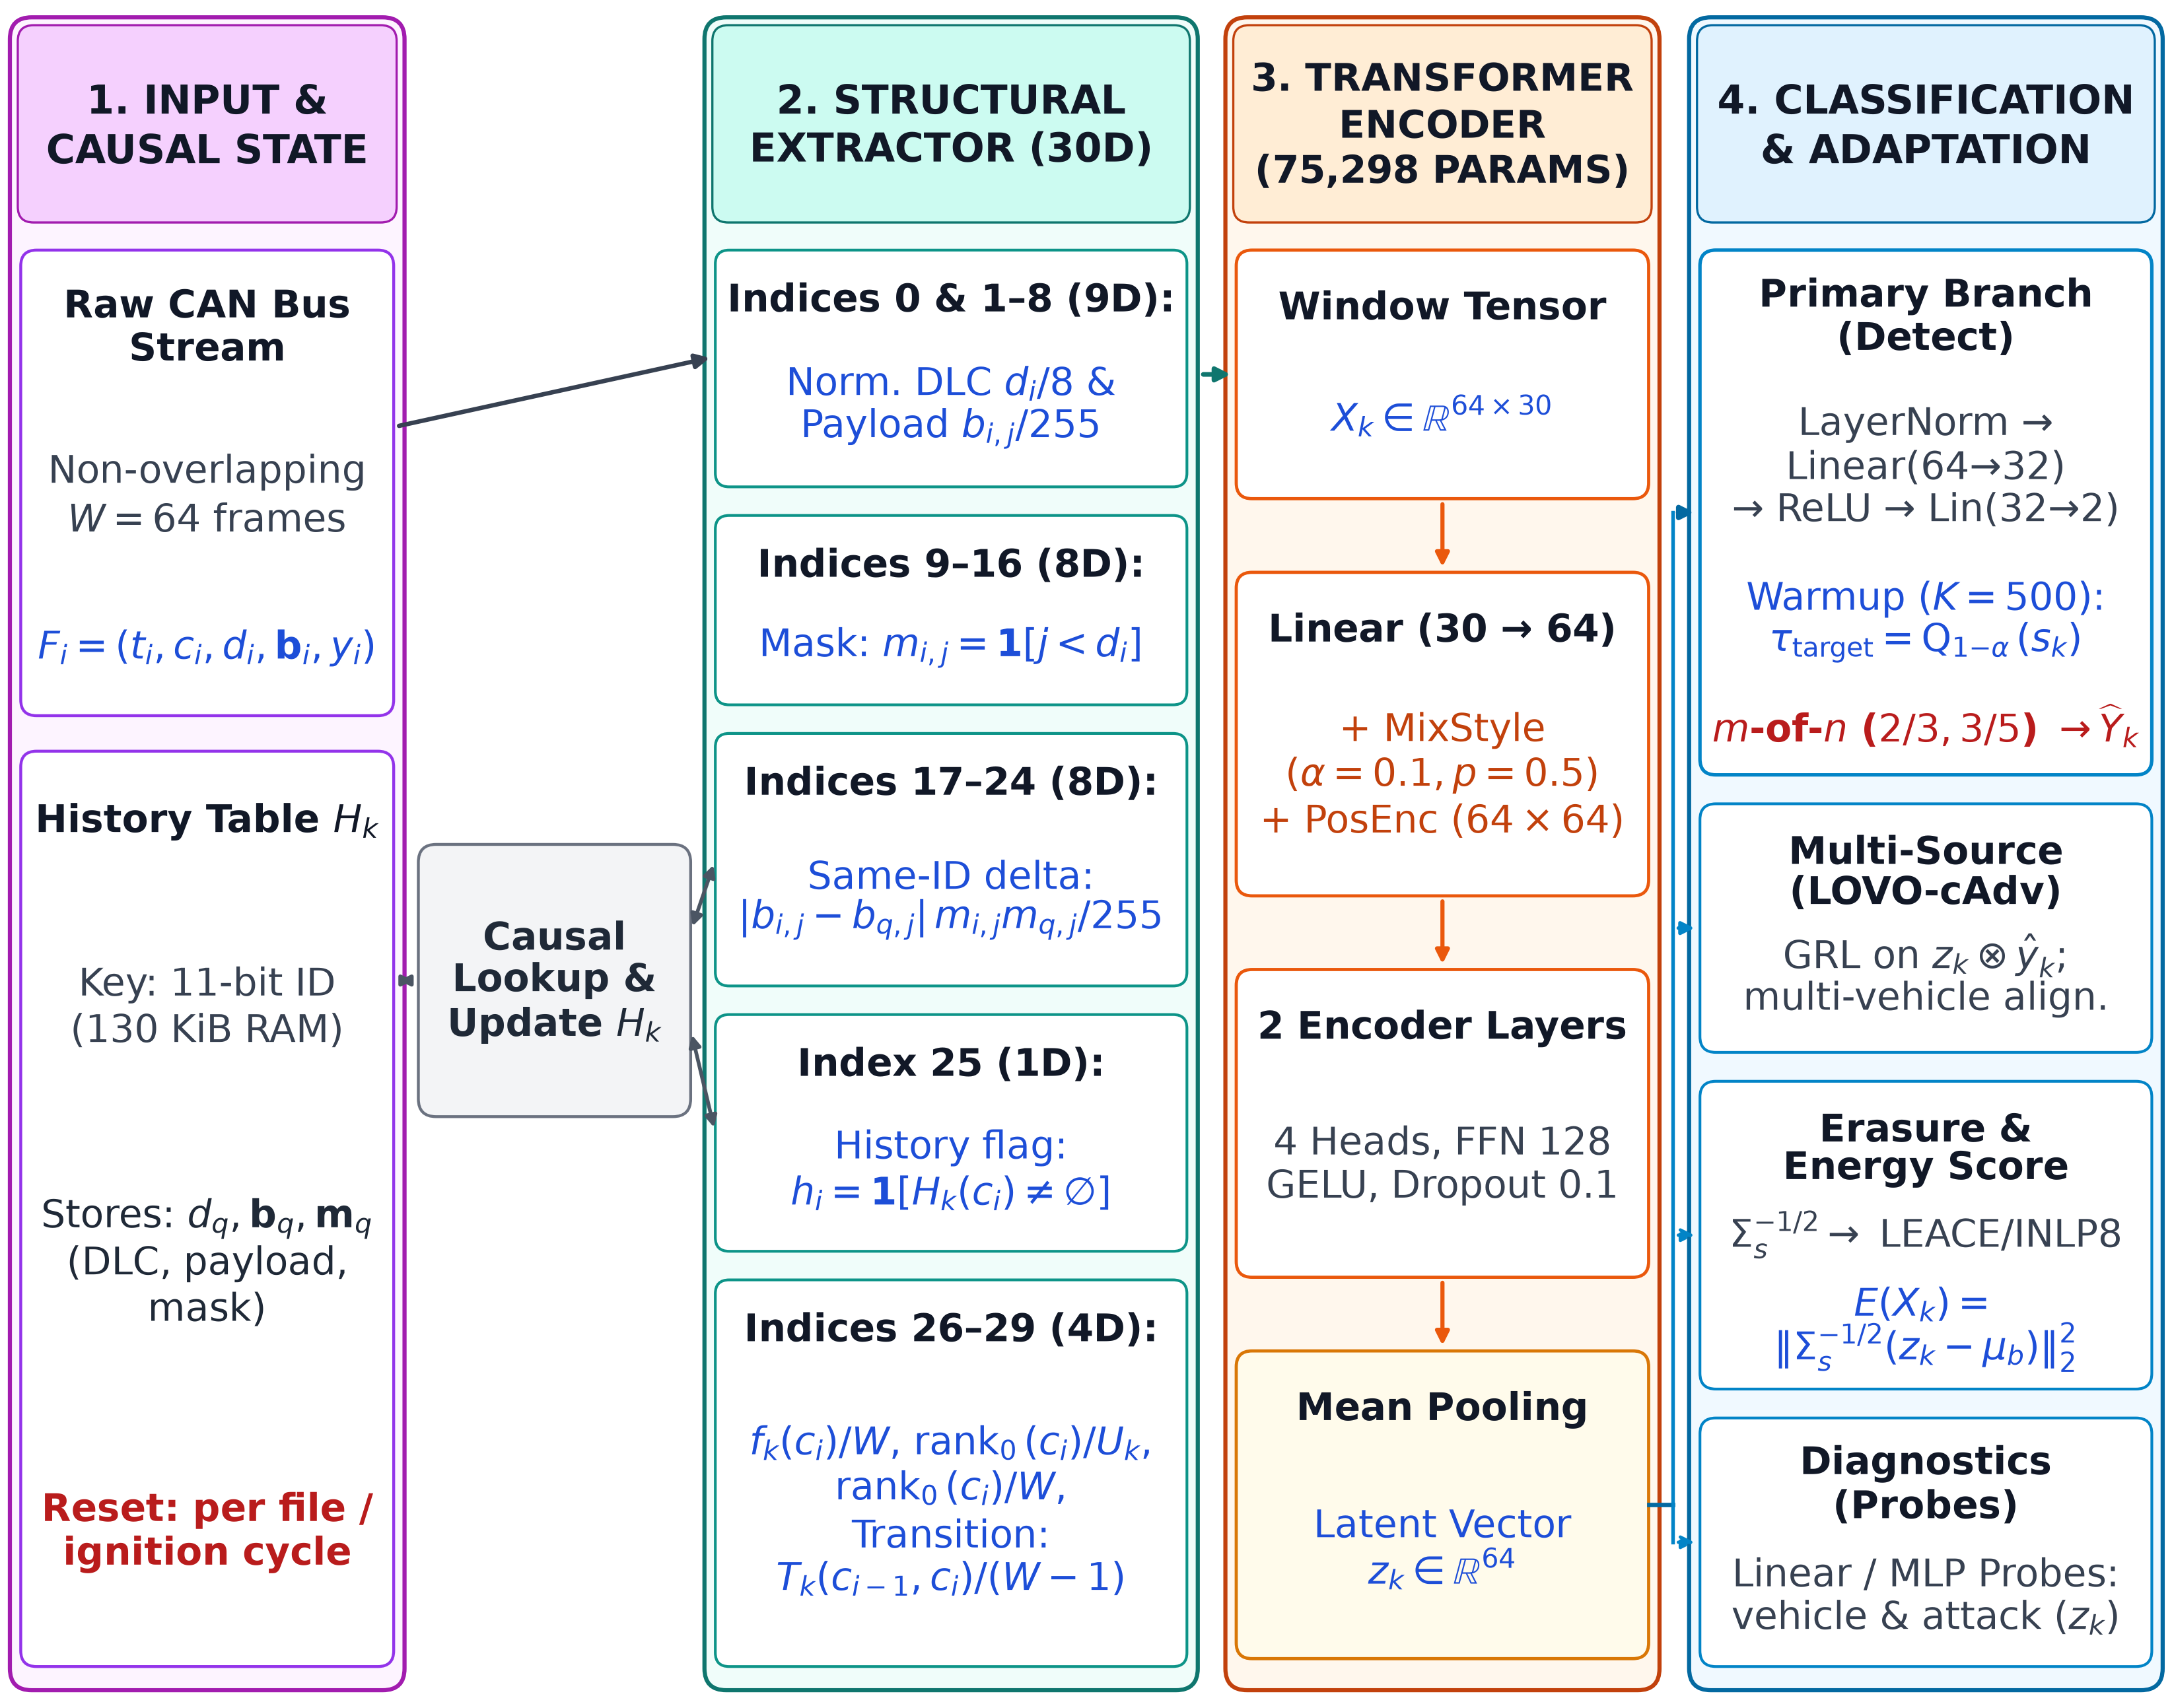
\includegraphics[width=0.98\textwidth]{figs/pipeline_architecture_30d.png}
\caption[Overall architecture of the Structural Transformer and adaptation pathways]{Overall architecture of the Structural Transformer method, adaptation extensions, and diagnostic pathways: (1) Raw CAN input stream ($W=64$) with causal lookup and updates against persistent history table $H_k$; (2) Frame-level 30D structural feature extraction; (3) 2-layer Transformer encoder ($75{,}298$ parameters) integrating MixStyle and mean pooling to form window representation $z_k \in \mathbb{R}^{64}$; (4) Primary classification branch with unsupervised benign warmup calibration ($K=500$) and sliding $m$-of-$n$ event filtering, alongside multi-source LOVO-cAdv DANN adaptation, benign covariance whitening with LEACE/INLP8 linear erasure and Mahalanobis energy scoring, and controlled diagnostic probes.}\label{fig:architecture-30d}
\end{figure}

Cross-entropy constrains predictions on training examples; it does not force every unseen attack into the benign class. Poor C/D performance may reflect attack coverage, representation, distribution shift or threshold choice. Without controlled evidence, observed limitations under Conditions C and D cannot be attributed solely to the cross-entropy loss, nor can reconstruction be guaranteed to resolve them. Detailed training hyperparameters and validation FAR budgets are specified in Section~\ref{sec:comparison-protocol} (Table~\ref{tab:config}).

\section{Domain adaptation and operational calibration extensions}\label{sec:domain-adaptation-methods}
To address distribution drift across vehicle models (particularly benign logit shift inducing source-threshold degradation), the thesis explores four post-hoc domain adaptation and vehicle-invariance mechanisms:

\subsection{Batch-Level Feature Statistics Mixing (MixStyle)}\label{subsec:method-mixstyle}
To enhance domain generalization without requiring target labels, MixStyle~\cite{zhou2021mixstyle} is adapted for the CAN Transformer encoder. During training, for pairs of inputs $(X, \widetilde{X})$ sharing the same window label ($Y = \widetilde{Y}$), frame-wise feature mean and standard deviation are computed after input projection ($E \in \mathbb{R}^{W \times d}$, with $d=64$) and prior to positional encoding:
\begin{equation}
\mu(X) = \frac{1}{W}\sum_{i=1}^W E_i, \qquad \sigma(X) = \sqrt{\frac{1}{W}\sum_{i=1}^W (E_i - \mu(X))^2 + \epsilon}.
\end{equation}
Mixed feature statistics are formed via convex interpolation:
\begin{align}
\gamma &= \lambda \sigma(X) + (1 - \lambda) \sigma(\widetilde{X}),\\
\beta &= \lambda \mu(X) + (1 - \lambda) \mu(\widetilde{X}),
\end{align}
where $\lambda \sim \text{Beta}(\alpha, \alpha)$ with $\alpha = 0.1$. The normalized feature representation becomes:
\begin{equation}
\operatorname{MixStyle}(X) = \gamma \odot \frac{E - \mu(X)}{\sigma(X)} + \beta.
\end{equation}
This perturbation activates with probability $p=0.5$ during training; at inference, the model operates deterministically (identity).

\subsection[Unsupervised Benign Warmup Calibration and Sliding m-of-n Event Filtering]{Unsupervised Benign Warmup Calibration and Sliding \texorpdfstring{$m$-of-$n$}{m-of-n} Event Filtering}\label{subsec:method-calibration}
To resolve the threshold shift on unseen vehicles without requiring attack labels, warmup calibration utilizes an initial prefix of $K$ benign windows observed upon vehicle startup. To strictly eliminate lookahead bias, the warmup boundary is capped at:
\begin{equation}
K_{\text{valid}} = \min\big(K, \lfloor \text{prefix\_end} / 2 \rfloor\big), \qquad K \in \{200, 500, 1000\}.
\end{equation}
The operational target threshold is computed via sample quantiles under a target FAR budget $\alpha \in \{0.1\%, 0.5\%, 1.0\%, 2.0\%\}$:
\begin{equation}
\tau_{\text{target}} = \operatorname{Quantile}_{1-\alpha}\big([s(X_k)]_{k=0}^{K_{\text{valid}}-1}\big).
\end{equation}
Furthermore, to suppress hourly false alarms on high-rate buses ($1{,}000\text{--}2{,}000\text{ frames/s}$), a sliding $m$-of-$n$ event filter is applied to post-warmup windows ($k = K_{\mathrm{valid}}, \ldots, M - 1$):
\begin{equation}\label{eq:mofn-filter}
\widehat{Y}_k^{(m/n)} = \mathbf{1}\!\left[\sum_{j=\max(K_{\mathrm{valid}},\, k-n+1)}^{k} \mathbf{1}\big[s(X_j) \ge \tau_{\mathrm{target}}\big] \ge m\right],
\end{equation}
triggering an intrusion alert only if at least $m$ of up to $n$ consecutive windows ($m/n \in \{2/3, 3/5\}$) exceed $\tau_{\text{target}}$. The complete leakage-free calibration and causal $m$-of-$n$ filtering procedure is specified in Algorithm~\ref{alg:benign-cal-mofn} (with $\mathrm{prefix\_end}$ denoting the count of initial benign windows prior to the first attack window, unified 0-based indexing $k=0,\ldots,M-1$ with Algorithm~\ref{alg:causal-30d}, and $s(X_k) = p_k = \operatorname{softmax}(f_\theta(X_k))_1$). Quantile computation over $K_{\mathrm{valid}} \le 1{,}000$ scalars incurs $\mathcal{O}(K_{\mathrm{valid}}\log K_{\mathrm{valid}})$ once post-warmup, while the sliding filter maintains only a ring buffer of capacity $n$ windows.

\begin{algorithm}[htbp]
\caption{Leakage-free unsupervised benign warmup calibration ($K_{\mathrm{valid}}$) and sliding $m$-of-$n$ event filtering}\label{alg:benign-cal-mofn}
{\small\linespread{1.05}\selectfont
\begin{algorithmic}[1]
\Require Frozen source classifier $f_\theta$ (fixed weights $\theta$); 0-based target capture windows $\{\mathcal{W}_k\}_{k=0}^{M-1}$ (initial benign prefix length $\mathrm{prefix\_end} \in \{0,\ldots,M\}$); warmup budget $K \in \{200, 500, 1000\}$; target FAR budget $\alpha \in \{0.1\%, 0.5\%, 1.0\%, 2.0\%\}$; sliding filter parameters $(m, n)$ (e.g., $2/3, 3/5$; default $(1,1)$ without filtering).
\Ensure Target operating threshold $\tau_{\mathrm{target}}$ and post-warmup decisions $\{\widehat{Y}_k^{(m/n)}\}_{k=K_{\mathrm{valid}}}^{M-1}$.
\State \textbf{Stage 1 --- Score extraction and leakage-free benign prefix collection:}
\State $H_0 \leftarrow \emptyset$; \quad $\mathcal{S}_{\mathrm{warm}} \leftarrow [\,]$ \Comment{Multiset preserving duplicate scalar scores}
\State $K_{\mathrm{valid}} \leftarrow \min\big(K,\, \lfloor \mathrm{prefix\_end} / 2 \rfloor\big)$ \Comment{Reserve at least half of benign prefix for evaluation}
\For{$k = 0$ \textbf{to} $M - 1$}
    \State $X_k, H_{k+1} \leftarrow \Phi(\mathcal{W}_k; H_k)$ \Comment{Invoke Algorithm~\ref{alg:causal-30d}}
    \State $s(X_k) \leftarrow p_k = \operatorname{softmax}(f_\theta(X_k))_1$ \Comment{Anomaly score from frozen $f_\theta$}
    \If{$k < K_{\mathrm{valid}}$}
        \State $\mathcal{S}_{\mathrm{warm}} \leftarrow \mathcal{S}_{\mathrm{warm}} \sqcup [s(X_k)]$ \Comment{Collect warmup scores ($0 \le k < K_{\mathrm{valid}}$)}
    \EndIf
\EndFor
\State \textbf{Stage 2 --- Target quantile threshold calibration:}
\State $\tau_{\mathrm{target}} \leftarrow \operatorname{Quantile}_{1-\alpha}(\mathcal{S}_{\mathrm{warm}})$ \Comment{Ensure $K_{\mathrm{valid}} \ge 1$ via same-vehicle pooling if needed}
\State \textbf{Stage 3 --- Post-warmup inference and sliding $m$-of-$n$ event filtering:}
\State Initialize binary alert buffer $a_k \leftarrow 0$ for $k = K_{\mathrm{valid}}, \ldots, M - 1$
\For{$k = K_{\mathrm{valid}}$ \textbf{to} $M - 1$}
    \State $a_k \leftarrow \mathbf{1}\big[s(X_k) \ge \tau_{\mathrm{target}}\big]$ \Comment{Raw window decision at index $k$}
    \State $j_0 \leftarrow \max(K_{\mathrm{valid}},\, k - n + 1)$ \Comment{Causal sliding window of at most $n$ steps}
    \State $c_k \leftarrow \sum_{j=j_0}^{k} a_j$ \Comment{Exceedance count within last $n$ windows}
    \State $\widehat{Y}_k^{(m/n)} \leftarrow \mathbf{1}[c_k \ge m]$ \Comment{Raise alert when at least $m$ of $n$ exceed}
\EndFor
\State \Return $\tau_{\mathrm{target}}, \{\widehat{Y}_k^{(m/n)}\}_{k=K_{\mathrm{valid}}}^{M-1}$
\end{algorithmic}}
\end{algorithm}

\subsection[Multi-Source LOVO with Conditional Adversarial Classifier]{Multi-Source Leave-One-Vehicle-Out Learning with Conditional Domain Adversarial Classifier (LOVO-cAdv DANN)}\label{subsec:method-lovo}
When multi-source data are available, Leave-One-Vehicle-Out (LOVO) cross-validation integrates a Domain-Adversarial Neural Network (DANN)~\cite{ganin2016dann}. Comprising feature extractor $G_f(\cdot; \theta_f)$, label classifier $G_y(\cdot; \theta_y)$, and domain discriminator $G_d(\cdot; \theta_d)$, the discriminator receives the conditional tensor product $z_k \otimes \hat{y}_k$ through a Gradient Reversal Layer (GRL):
\begin{equation}
\mathcal{L}_{\text{total}} = \mathcal{L}_y(G_y(G_f(X)), Y) - \lambda_{\text{adv}} \mathcal{L}_d\big(G_d(\operatorname{GRL}_{\lambda}(z \otimes \hat{y})), V\big),
\end{equation}
where $V$ denotes source-vehicle identity and $\lambda_{\text{adv}}$ follows an ascending training schedule to encourage vehicle-invariant representations.

\subsection[Benign Covariance Whitening, LEACE/INLP8, and Energy Scoring]{Benign-Target Covariance Whitening, Linear Concept Erasure (LEACE/INLP8), and Mahalanobis Energy Scoring}\label{subsec:method-whitening}
To investigate vehicle-identity remnants in the frozen 64-dimensional embedding space $z_k \in \mathbb{R}^{64}$, a three-stage geometric purification framework is established:
\begin{enumerate}
    \item \textbf{Benign-Target Covariance Whitening:} From 1,000 even-indexed benign windows of the target vehicle, sample mean $\mu_b$ and shrinkage covariance $\Sigma_s = (1-\gamma)\Sigma_b + \gamma \bar{\sigma}^2 I$ ($\gamma = 0.1$) are estimated. The whitening transformation $W_{\text{white}} = \Sigma_s^{-1/2}$ maps embeddings to $z'_k = W_{\text{white}}(z_k - \mu_b)$, standardizing target benign variance.
    \item \textbf{Linear Concept Erasure:} Orthogonal projections via LEACE~\cite{belrose2023leace} or Iterative Nullspace Projection (INLP8, 8 iterations)~\cite{ravfogel2020null} fitted exclusively on source vehicles eliminate linear vehicle subspaces.
    \item \textbf{Mahalanobis Energy Scoring (\code{white\_energy}):} Bypassing the source classification head, an anomaly energy score is evaluated directly on the whitened embedding:
    \begin{equation}
    E(X_k) = \| W_{\text{white}} (z_k - \mu_b) \|_2^2,
    \end{equation}
    yielding a metric-based anomaly detector calibrated entirely against target benign dynamics.
\end{enumerate}

\section{Chapter summary}
This chapter specified the window-level problem formulation, data validation contracts, causal history table management, 30-dimensional structural representation with causal extraction (Algorithm~\ref{alg:causal-30d}), Transformer sequence encoder, leakage-free unsupervised benign warmup calibration with sliding $m$-of-$n$ filtering (Algorithm~\ref{alg:benign-cal-mofn}), and domain adaptation extensions. Chapter~\ref{chap:results} establishes the experimental protocol and presents quantitative empirical evaluations.

\chapter{Experiments and evaluation}\label{chap:results}
This chapter distinguishes the primary criterion from additional post-hoc analyses. Aggregation averages seeds within sets before equally weighting sets; windows are not independent vehicles. A dash means undefined, not zero. Section 4.1 defines the experimental setup and protocol; Section 4.2 evaluates zero-shot transfer and representation diagnostics (RQ1--RQ4); Section 4.3 evaluates domain adaptation and operational calibration recovery; and Section 4.4 examines workstation processing latency and threats to validity.

\section{Experimental setup and protocol}
\subsection{Source splitting, sampling and leakage control}
Table~\ref{tab:split-stats} summarizes the recording-round split structure across the four datasets following input integrity verification: in total, 30 source training files ($388{,}435$ completed $W=64$ windows; recording-round suffixes 1 and 3) and 30 source validation files ($385{,}168$ full unsubsampled $W=64$ windows; suffixes 2 and 4) are held strictly disjoint from test conditions A--D during both training and threshold selection.

{\renewcommand{\arraystretch}{0.88}
\begin{table}[htbp]\centering\footnotesize
\caption{Source train/validation split statistics, test capture counts, and attack-family distributions across the four \texttt{can-train-and-test} sets}\label{tab:split-stats}
\begin{tabular}{P{1.1cm}P{2.2cm}P{2.2cm}P{1.5cm}P{6.3cm}}
\toprule
Set & Source (Train/Val) & Test A/B/C/D & Val Suffixes & Attack Families in A--B / C--D \\ \midrule
1 & 6 / 6 files & 8 / 8 / 12 / 12 & 2, 4 & A--B: DoS, force-neutral, rpm, standstill; C--D: double, fuzzing, interval, speed, systematic, triple \\
2 & 8 / 8 files & 12 / 12 / 8 / 8 & 2, 4 & A--B: double, fuzzing, interval, speed, systematic, triple; C--D: DoS, force-neutral, rpm, standstill \\
3 & 7 / 7 files & 10 / 10 / 14 / 14 & 2, 4 & A--B: DoS, double, force-neutral, fuzzing, triple; C--D: interval, rpm, rpm-acc., speed, speed-acc., standstill, systematic \\
4 & 9 / 9 files & 14 / 14 / 10 / 10 & 2, 4 & A--B: interval, rpm, rpm-acc., speed, speed-acc., standstill, systematic; C--D: DoS, double, force-neutral, fuzzing, triple \\
\bottomrule
\end{tabular}
\end{table}}

Source files are grouped by their trailing recording-round number, keeping all files with the same suffix together. The highest-numbered group is the default validation group. This is more conservative than random-window splitting, but metadata are still needed to establish independent driving sessions. The model is not refitted using validation after threshold selection, because that would break correspondence between checkpoint and threshold.

Sampling bounds memory through separate random-priority reservoirs for each file and class. Every window receives a random key; the smallest 1,000 keys per class are retained. The complete file is read before selection is finalized. An attack near the end therefore has the same selection opportunity as an early attack. Sampling occurs after continuous-state feature extraction, never by assembling disconnected frames into artificial sequences.

Selected window indices and available/selected counts by class and file are exported. All representations share the same sample. Validation and tests retain their natural prevalence and are evaluated in full. Attack-family coverage is retained to inspect classes and mechanisms in the actual source sample.

The executed sampler uses separate random streams per file and class, seeded from the sampling seed and filename. Changing chunksize or file traversal order therefore preserves a file's selected windows. Saved sample indices ensure all methods in a comparison use the same source windows.

Research runs require a successful full-file preflight manifest matching the validator specifications, documented input exclusions, and current SHA-256 data hashes. Preflight requires all four sets and A--D folders, records missing/excluded external files separately, and detects identical files involving source data within a set. SHA-256 does not rule out shared trace segments or establish independent driving sessions; session provenance remains a limitation to verify.

\subsection{Comparators, training configuration and the CTT evaluation protocol}\label{sec:comparison-protocol}
Table~\ref{tab:config} summarizes the default experimental training hyperparameters and the validation FAR budget used for source threshold selection ($100$ per $100{,}000$ benign windows, serving as a benchmark comparison design choice rather than an automotive safety standard). Logistic regression (LR) is used solely for post-hoc linear probing rather than as a ranked IDS comparator.

{\renewcommand{\arraystretch}{0.88}
\begin{table}[htbp]\centering\footnotesize
\caption{Default experimental training hyperparameters and validation false-alarm budget}\label{tab:config}
\begin{tabular}{ll}\toprule Parameter & Value\\\midrule
Main window / sensitivity & 64 / 32 and 128\\
Hidden / layers / heads & 64 / 2 / 4\\
Feed-forward / dropout & 128 / 0.1\\
Optimizer & AdamW\\
Learning rate / weight decay & 0.001 / $10^{-4}$\\
Epochs / batch size & 10 / 128\\
Scheduler & Epoch-wise cosine\\
Initialization seeds & 42, 43, 44\\
Shared sampling seed & 20261103\\
Training cap per file and class & 1,000 windows\\
Validation FAR budget & 100 per 100,000 benign windows\\\bottomrule\end{tabular}
\end{table}}

\textbf{The executing protocol is \code{ctt-content-order-comparison-v1}.}
Scanning all 236 CTT files identified 193,240,845 data frames (differing by 236 header lines from 193,241,081 CSV lines), 3,019,271 completed W64 repository windows, and 12,527 timestamp decreases across 100 files. Consequently, the primary 60-unit IDS matrix (4 sets $\times$ 3 seeds $\times$ 5 methods) strictly uses content and file order (Raw 28D and Structural 30D; SHA-256 manifest hashes recorded in Appendix~\ref{sec:app-provenance}), while isolating the extended timing-aware specification (Timed 29D/32D) into an independent sensitivity control over the 136 strictly monotonic files in Appendix~\ref{app:sensitivity}.

The cache retains original IDs, DLCs, payloads, labels, timestamps and row order without sorting, deduplication or synthetic time. The content-only schema omits all timing dimensions to retain 28 raw and 30 structural dimensions as indexed in Table~\ref{tab:features}. History features follow file order and are not interpreted as physical transmission periods. Four sets, seeds 42/43/44 and five methods form 60 IDS units, each evaluated on A--D. CANBERT+ pretraining and fine-tuning are two phases within one unit. W64 windows do not overlap or cross files. Full-file reservoir sampling selects at most 1,000 windows per class per source training file, with sampling seed 20261103 and identical source-window indices across methods. Source validation is grouped by recording-round suffix; vocabularies, TF-IDF and all learned parameters use source data only.

\subsubsection{Comparators, supervision and departures from publications}
Raw and Structural Transformer share encoder architecture, source samples, CE/AdamW/Cosine, 10 epochs, batch 128 and learning rate 0.001; their principal difference is the 28/30-dimensional representation. This comparison tests the representation package and does not isolate identifier removal from each added structural feature.

CANBERT+~\cite{won2026canbertplus} imports the authors' BERT/MLM modules with hidden size 768, six layers and 12 heads. The vocabulary is source-only; benign-source pretraining masks 15\% of identifiers for three epochs, followed by three epochs of frame-supervised fine-tuning with batch eight. Replacing Lightning with a PyTorch loop, shared sampling, grouped splits, W64, fixed epochs and ensuring at least one masked token per batch are disclosed adaptations. The window score is the maximum frame score ($\max_{i\in\mathcal{W}_k} s_i$) and does not measure frame localization. While aligning the evaluation unit, this maximum aggregation compounds frame-level false-positive probabilities across 64 frames, shifting validation scores upward and driving the source-calibrated threshold to stringent values.

CANLP~\cite{balasubramanian2025canlp} is adapted to character TF-IDF unigrams, at most 256 bigrams and ID/2048, followed by Dense 128/64, dropout 0.15 and two output classes. The PyTorch port uses Adam 0.001, batch 512, 30 epochs, original frame labels and maximum score/W64. TF-IDF fits only frames within sampled source-training windows. Grouped source splits, no deduplication, binary labels and fixed epochs replace the original publication's checkpoint selection; the reported name is CANLP-char-DNN adapted.

CrySyS-AssocRules/W64 imports the association-rule implementation from the framework~\cite{koltai2026trust}, fitting benign source data only. Window/stride 64/64 replaces the reference implementation's 900/450; relations never bridge gaps between selected samples. Default cluster count 300, distance threshold 0.3 and maximum itemset sizes three for fitting and two for scoring are retained. This is a framework-derived adapted comparator, not a claim to reproduce a different similarly named method unchanged. Pinned source commits of competitor implementations are recorded in Appendix~\ref{sec:app-provenance}.

Supervision and compute budgets differ: the Transformers use window labels; CANBERT+ additionally uses benign pretraining and frame labels; CANLP uses frame labels; AssocRules uses benign traffic only. This compares complete pipelines under shared data/evaluation rules, not equal-budget ablations or original published scores. Adaptation qualifiers remain visible in result tables.

\noindent\textbf{Thresholds, pairing, acceleration, and interpretation limits:} Source validation selects the threshold maximizing recall under a FAR budget of 100 per 100,000 benign source windows. Target labels never calibrate the threshold, and target FAR may exceed the budget. Paired differences subtract each opponent from Structural within each set and seed, averaging seeds within a set before equally weighting the four sets. Paired bootstrap resamples entire capture files and recomputes metrics from confusion counts, describing conditional variation over observed files rather than population-level vehicle confidence intervals. Four neural methods execute on an RTX 5060, while AssocRules uses an exact-call CPU cache backend preserving native fitting/scoring (a source-only $k=2$ validation check matched scores, rules, and centroids exactly with $\sim 8.3\times$ speedup; reservoir subsampling at $W=64$ increases itemset sparsity and drives rare legitimate validation transitions to score $1.0$). Four completed GPU Set~1/seed~42 cells are retained after verifying hashes, environment, and configuration. Seeds and environment are recorded, though CUDA attention exhibits minor hardware-level GPU nondeterminism; three seeds capture observed run variation without creating independent vehicles.

\subsection{Thresholds, metrics and controlled diagnostic design}
The default 0.5 threshold is reported alongside a source-calibrated threshold. Calibration maximizes validation recall subject to an observed FAR budget, breaking ties toward fewer false positives and then a higher threshold. Equal scores are treated together rather than arbitrarily split. A threshold above the maximum score is feasible when no positive decision satisfies the constraint; its zero recall must be disclosed.

For $N_+=TP+FN$ and $N_-=TN+FP$:
\begin{align}
P&=TP/(TP+FP), & R&=TP/N_+,\\
F_1&=2TP/(2TP+FP+FN), & \operatorname{FAR}_{100k}&=10^5FP/N_-.
\end{align}
FAR is N/A when $N_-=0$. Without positive ground truth, attack metrics are not interpreted as detection evidence. Precision is N/A when no alerts exist; with positive examples but no detections, recall and F1 are zero. AP uses continuous scores when both classes are present. It is never replaced by F1 when scores or a class are absent. The area under the Precision--Recall curve (PR-AUC) is evaluated consistently via Average Precision (AP), capturing the step-weighted mean precision across thresholds rather than a trapezoidal approximation.

The selected source threshold remains fixed for A--D and compatible external tests. Its source FAR budget does not guarantee target FAR. The smallest empirical FAR increment is $10^5/N_-$; sample counts must therefore accompany low-FAR claims, especially for small validation sets. Table~\ref{tab:ablations} summarizes the 10 controlled ablation comparisons and their corresponding research objectives.

{\renewcommand{\arraystretch}{0.88}
\begin{table}[htbp]\centering\footnotesize
\caption{Summary of controlled ablation comparisons and their corresponding research objectives}\label{tab:ablations}
\begin{tabular}{P{4.6cm}P{9.2cm}}
\toprule
Comparison & Purpose\\\midrule
Raw vs raw-minus-ID & Isolate removal of 11 original ID bits\\
Raw-plus-structural vs raw & Add history/structure while retaining IDs\\
Structural vs raw-plus-structural & Test IDs with a richer feature set\\
Structural-minus-delta & Payload changes and history flag\\
Structural-minus-local & Local frequency and rank\\
Structural-minus-transition & Bigram frequency\\
Structural-minus-payload & Remove absolute bytes; retain DLC/masks and history\\
Structural-minus-rank-W & Remove content dimension 28 only; retain other statistics\\
ID-only / raw-minus-ID & Content-modality limits; timing-only is not applicable\\
32/64/128 frames & Window sensitivity and waiting time\\\bottomrule
\end{tabular}
\end{table}}

Probes freeze the trained raw/structural encoders. Diagnostic data are split by capture group and balanced across vehicle-by-attack cells within each partition, reducing vehicle prediction from attack prevalence alone. LR predicts vehicle or attack from embeddings. Probes are post-freeze diagnostics, not target-informed checkpoint or threshold selection. Balanced chance accuracy is $1/V$ for $V$ vehicles. Probe results include constant/random embeddings as controls for decoder capacity~\cite{hewitt2019probes} and an attack probe to determine whether reduced vehicle information also removes useful detection signal. Probes use LR with $C=1$, at most 2,000 iterations and scaling fitted on probe training data; randomized controls use five fixed seeds.

\subsection{Reproducibility and computational cost protocol}
The run manifest stores schema version, configuration, Python/library versions, device and code hashes. The data manifest stores relative paths, sizes and full-file SHA-256. Every checkpoint records its dimensions, window size and threshold; prediction files retain window indices, labels, scores and start/end timestamps. To guarantee experimental immutability, artifact storage enforces read-only artifact locking preventing accidental overwriting of completed run directories.

Attention cost grows quadratically with $W$, while local statistics and history updates are linear in frame count. Runtime evaluation must include parsing, feature extraction, inference and window waiting time. GPU batch throughput alone is not online latency. The final manifest hashes checkpoints, metadata, metrics and prediction files; aggregation rejects incomplete runs, altered outputs, incompatible code/protocols, and repeated/missing set--seed--model cells. The execution orchestrator verifies and skips compatible completed units, while interrupted runs are restarted in new directories rather than resumed from a partial epoch.

Content runtime is measured separately on a source-validation prefix on an experimental workstation equipped with an AMD Ryzen 5 5600X CPU (6 cores/12 threads @ 3.7 GHz, 16 GB DDR4 RAM) and an NVIDIA GeForce RTX 5060 GPU (8 GB VRAM, Windows 11 host): batch one, 20 warmup windows and 300 measured windows over three repetitions. It includes CSV reading, conversion/validation, both representations and inference. Acquisition waits and event-level latency are not measured; results do not certify ECU deadlines.

\section{Zero-shot transfer and representation diagnostics}
\subsection{Detection performance and false alarm evaluation under vehicle transfer (RQ1)}\label{sec:comparison-results}
Table~\ref{tab:comparison-main} reports the primary five-method benchmark at window size $W=64$ under frozen source thresholds (shared test-window denominators are detailed in Table~\ref{tab:comparison-counts}, Appendix~\ref{app:sensitivity}), while Table~\ref{tab:comparison-paired} summarizes paired differences in Conditions B and D. B tests an unseen vehicle with known attacks; D changes both vehicle and attack type. Source thresholds remain frozen; the source budget of 100/100,000 does not bound target FAR, and original published scores are not included in this table.

\Needspace{6\baselineskip}
{\footnotesize\renewcommand{\arraystretch}{0.85}
\begin{longtable}{P{1.0cm}P{4.4cm}P{1.4cm}P{3.0cm}P{1.4cm}P{1.4cm}}
\caption[Primary five-method comparison at W=64 under frozen source thresholds]{Primary five-method benchmark at window size $W=64$ under frozen source thresholds across Conditions A--D (FAR per 100,000 benign windows and equivalent percentage)}\label{tab:comparison-main}\\\toprule
Cond. & Method & Recall & FAR /100k (\%) & F1 & AP\\\midrule
\endfirsthead\caption[]{(continued)}\\\toprule
Cond. & Method & Recall & FAR /100k (\%) & F1 & AP\\\midrule
\endhead
A & Raw TF & 0.6167 & 115.77 (0.12\%) & 0.7258 & 0.7312\\
A & Structural TF & 0.5886 & 81.67 (0.08\%) & 0.7072 & 0.7483\\
A & CANBERT+ adapted & 0.3843 & 79.27 (0.08\%) & 0.4576 & 0.5335\\
A & CANLP-char-DNN adapted & 0.1228 & 28.37 (0.03\%) & 0.1789 & 0.5482\\
A & CrySyS-AssocRules/W64$^{\dagger}$ & 0.0000 & 0.00 (0.00\%) & 0.0000 & 0.3338\\
B & Raw TF & 0.8541 & 65301.41 (65.30\%) & 0.3000 & 0.3781\\
B & Structural TF & 0.7383 & 52461.46 (52.46\%) & 0.2435 & 0.5554\\
B & CANBERT+ adapted & 0.6395 & 64843.85 (64.84\%) & 0.0593 & 0.0970\\
B & CANLP-char-DNN adapted & 0.2854 & 29695.88 (29.70\%) & 0.0329 & 0.0542\\
B & CrySyS-AssocRules/W64$^{\dagger}$ & 0.0000 & 0.00 (0.00\%) & 0.0000 & 0.0591\\
C & Raw TF & 0.2101 & 91.92 (0.09\%) & 0.2314 & 0.2661\\
C & Structural TF & 0.2230 & 75.82 (0.08\%) & 0.2600 & 0.2928\\
C & CANBERT+ adapted & 0.1037 & 62.54 (0.06\%) & 0.1461 & 0.2218\\
C & CANLP-char-DNN adapted & 0.0020 & 405.49 (0.41\%) & 0.0038 & 0.2373\\
C & CrySyS-AssocRules/W64$^{\dagger}$ & 0.0000 & 0.00 (0.00\%) & 0.0000 & 0.1732\\
D & Raw TF & 0.6614 & 67982.89 (67.98\%) & 0.1213 & 0.1648\\
D & Structural TF & 0.6445 & 54643.37 (54.64\%) & 0.2069 & 0.3357\\
D & CANBERT+ adapted & 0.5549 & 54513.45 (54.51\%) & 0.0644 & 0.1311\\
D & CANLP-char-DNN adapted & 0.2491 & 25452.19 (25.45\%) & 0.0119 & 0.0901\\
D & CrySyS-AssocRules/W64$^{\dagger}$ & 0.0000 & 0.00 (0.00\%) & 0.0000 & 0.0912\\
\bottomrule
\multicolumn{6}{P{13.4cm}}{\footnotesize $^{\dagger}$ Source-validation threshold degenerates at $1.0000000000000002$ (all-benign prediction, $R=0, \text{FAR}=0$); see Section~\ref{subsec:assoc-degenerate} for details.}
\end{longtable}}

{\renewcommand{\arraystretch}{0.85}
\begin{table}[htbp]\centering\footnotesize
\caption[Paired performance differences between Structural and active neural opponents]{Paired performance differences between the Structural Transformer and active neural opponents in Conditions B and D (equal set weights, FAR per 100,000 windows and percentage points)}\label{tab:comparison-paired}
\begin{tabular}{P{1.1cm}P{4.7cm}P{1.6cm}P{2.8cm}P{1.4cm}P{1.4cm}}
\toprule
Cond. & Opponent & $\Delta R$ & $\Delta$ FAR /100k (\%pt) & $\Delta$ F1 & $\Delta$ AP\\\midrule
B & Raw TF & -0.1159 & -12839.95 (-12.84) & -0.0565 & 0.1774\\
B & CANBERT+ adapted & 0.0988 & -12382.39 (-12.38) & 0.1842 & 0.4584\\
B & CANLP-char-DNN adapted & 0.4529 & 22765.57 (+22.77) & 0.2106 & 0.5012\\
D & Raw TF & -0.0169 & -13339.51 (-13.34) & 0.0856 & 0.1709\\
D & CANBERT+ adapted & 0.0896 & 129.92 (+0.13) & 0.1425 & 0.2046\\
D & CANLP-char-DNN adapted & 0.3953 & 29191.18 (+29.19) & 0.1950 & 0.2456\\
\midrule
\multicolumn{6}{P{13.4cm}}{\footnotesize \textit{Degenerate comparator note:} \code{CrySyS-AssocRules/W64} is omitted from active paired differences because its source threshold degenerates at $1.0000000000000002$ ($\text{Recall}=0.0000, \text{FAR}=0.00$ across A--D); subtracting $0$ ($\Delta R = +0.7383$, $\Delta\text{FAR}=+52,461.46$ in B; $\Delta R = +0.6445$, $\Delta\text{FAR}=+54,643.37$ in D) is purely arithmetic rather than comparison against an active detector. On threshold-free AP, Structural outperforms CrySyS-AssocRules/W64 ($\Delta\text{AP}=+0.4964$ in B and $+0.2445$ in D).}\\
\bottomrule\end{tabular}
\end{table}}

\begin{figure}[htbp]
\centering
\begin{subfigure}[b]{0.45\textwidth}
  \centering
  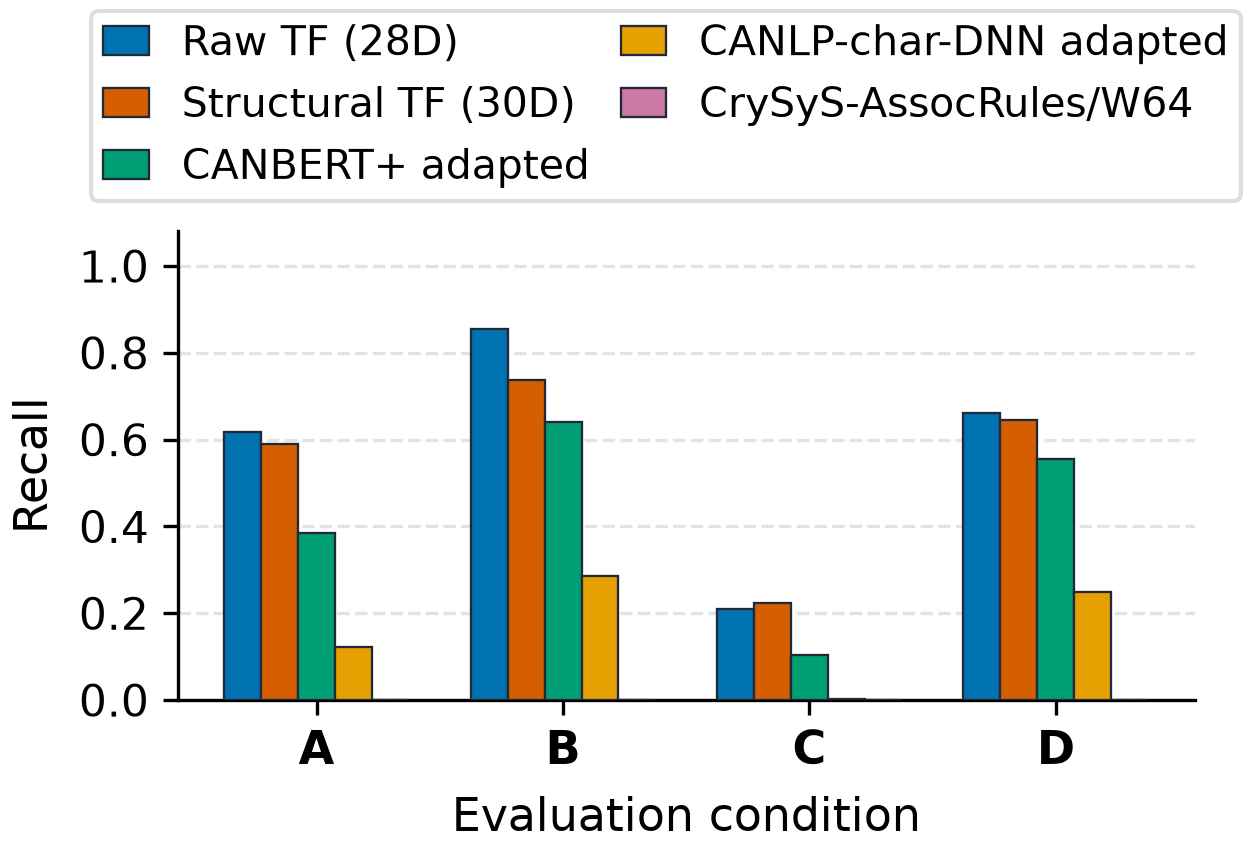
\includegraphics[width=\linewidth]{figs/comparison_v1_Recall.png}
  \caption{Recall}\label{subfig:comp-recall}
\end{subfigure}\hfill
\begin{subfigure}[b]{0.45\textwidth}
  \centering
  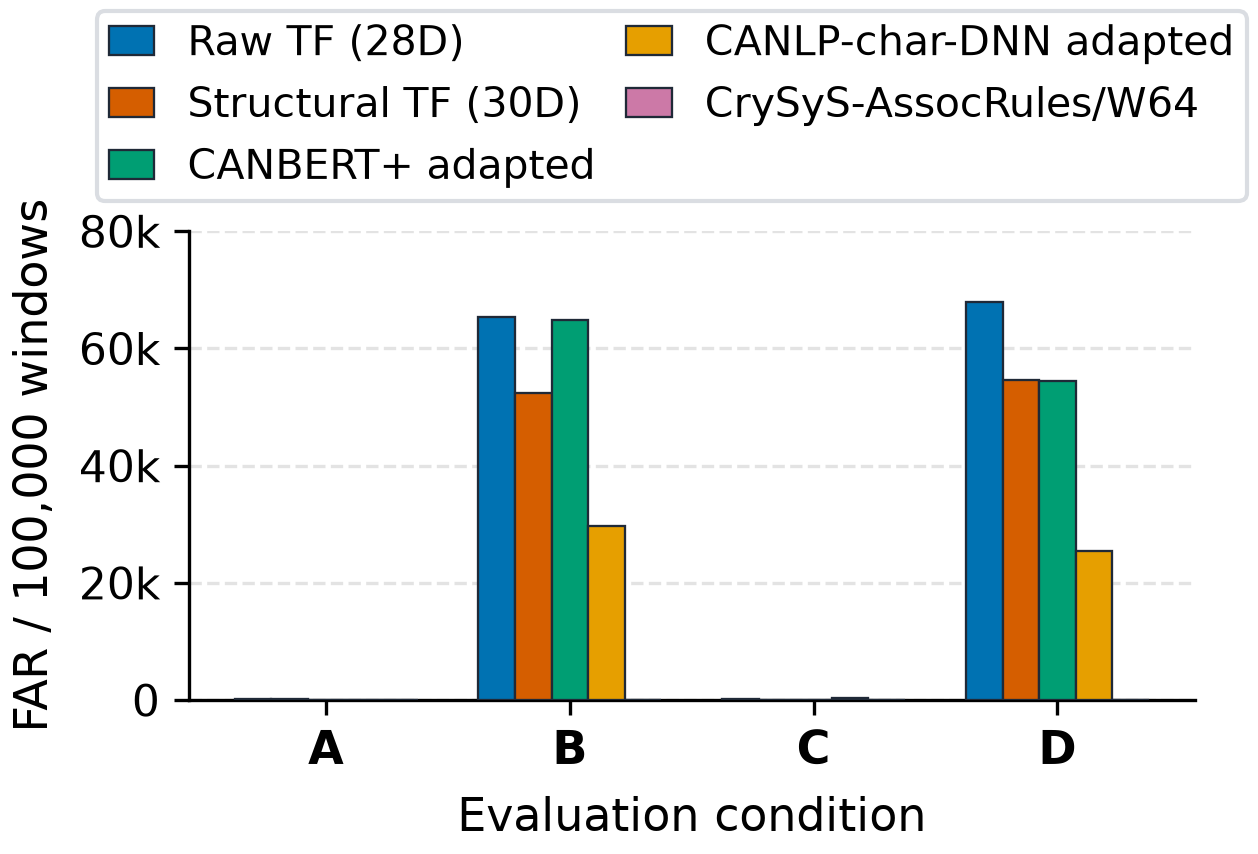
\includegraphics[width=\linewidth]{figs/comparison_v1_FAR_per_100k.png}
  \caption{FAR per 100,000 windows}\label{subfig:comp-far}
\end{subfigure}
\vskip 2pt
\begin{subfigure}[b]{0.45\textwidth}
  \centering
  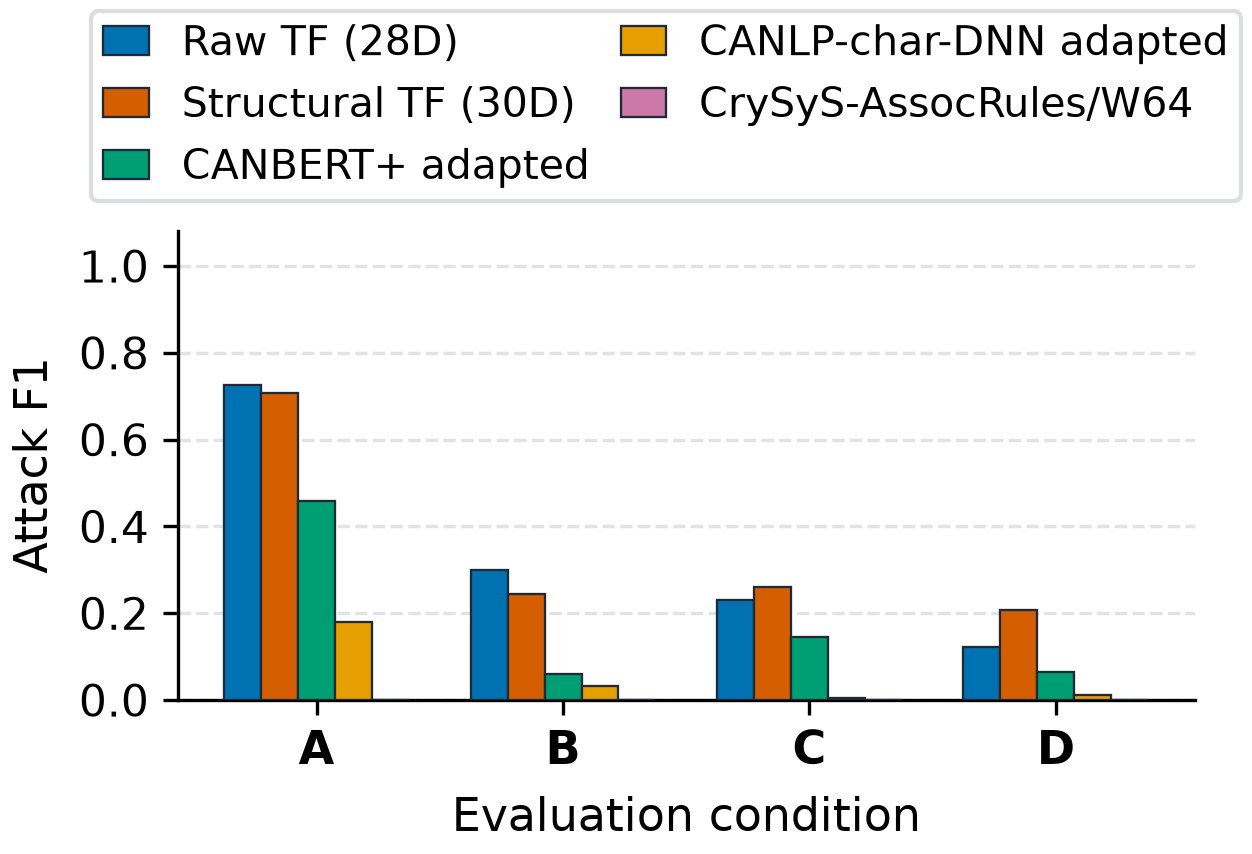
\includegraphics[width=\linewidth]{figs/comparison_v1_Attack_F1.png}
  \caption{Attack F1}\label{subfig:comp-f1}
\end{subfigure}\hfill
\begin{subfigure}[b]{0.45\textwidth}
  \centering
  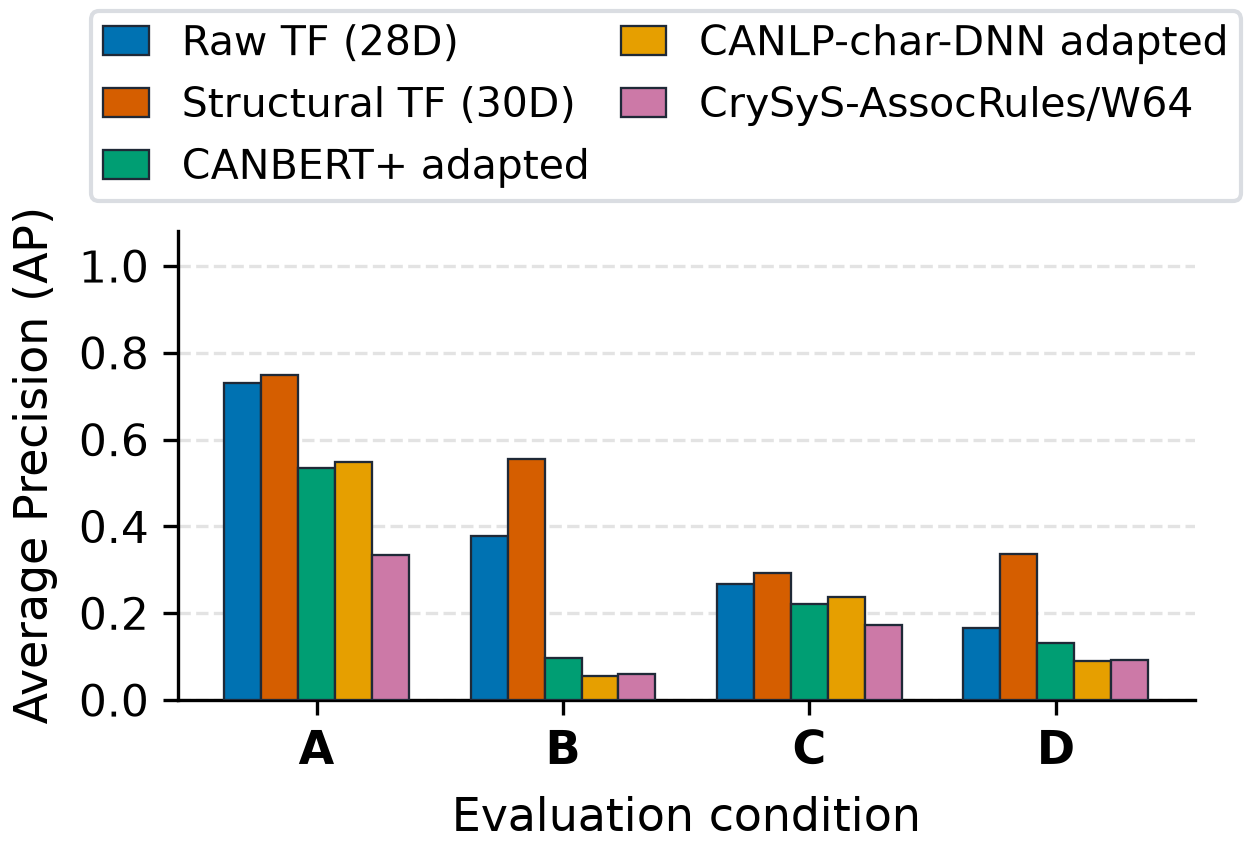
\includegraphics[width=\linewidth]{figs/comparison_v1_AP.png}
  \caption{Average Precision (AP)}\label{subfig:comp-ap}
\end{subfigure}
\caption[Five-method evaluation at W=64 across Conditions A--D]{Five-method evaluation at window size $W=64$ across Conditions A--D under frozen source thresholds (equal four-set weights).}\label{fig:comparison-four-metrics}
\end{figure}
\FloatBarrier

From Tables~\ref{tab:comparison-main}--\ref{tab:comparison-paired} and Figure~\ref{fig:comparison-four-metrics}, in B, Structural minus Raw recall is $-11.59$ percentage points ($0.7383$ vs $0.8541$), while the paired AP increase is $+0.1774$ ($+17.74$ percentage points paired difference; $+17.73$ percentage points difference of means, $0.5554 - 0.3781$). FAR falls by $12.84$ percentage points but remains $52.46\%$ ($52,461.46$ per 100k). In D under source thresholds, Structural achieves AP $0.3357$ (equal 4-set mean; $0.3404$ under 3-target-vehicle deduplication, compared to Raw $0.1648$ and $0.1799$), recall changes by $-1.69$ percentage points, and FAR remains $54.64\%$ ($43.60\%$ deduplicated); note that $\text{AP}_D=0.3411$ corresponds to post-warmup calibration at $K=500$ (Section~\ref{sec:benign-calibration}). Deduplicating Subaru Forester's target weight ($1/3, 1/6, 1/6, 1/3$) yields: in B, Structural achieves recall $0.6610$, FAR $41.26\%$, F1 $0.2891$, AP $0.5510$, whereas Raw achieves recall $0.8722$, FAR $60.23\%$, F1 $0.3629$, AP $0.4281$; in D, Structural achieves AP $0.3404$ (Raw $0.1799$) and FAR $43.60\%$ (Raw $63.69\%$). The primary increased-recall hypothesis for B is unsupported. Improved AP is a secondary ranking result and neither resolves high false alarms nor replaces the primary criterion.

Per-pair breakdown (detailed in Table~\ref{tab:comparison-sets} and Table~\ref{tab:comparison-ci} in Appendix~\ref{app:reproducibility}) reveals a sharp divergence between intra-manufacturer and cross-manufacturer transfer: in Set 1 (Chevrolet Impala to Chevrolet Silverado), Structural tightly controls target FAR at $32.14$ per 100,000 ($0.032\%$), substantially outperforming Raw ($168.99$ per 100,000), while Set~1 seed variance is large ($\pm 0.3875$). In Sets 2, 3 and 4 (Chevrolet--Subaru transfer), baseline scores drift past $\tau_{\text{source}}$, inflating target FAR to $37,700\text{--}100,000$ per 100,000, yet Structural achieves strictly superior AP over Raw on $4/4$ sets in Condition B.

\noindent\textbf{Timestamp monotonicity sensitivity verification:} Across the $136/236$ strictly monotonic CTT captures (detailed in Section~\ref{subsec:monotonic-sensitivity} and Table~\ref{tab:monotonic-timed-vs-content}, Appendix~\ref{app:sensitivity}), \code{Timed Structural (32D)} achieves $\text{AP}_B=0.9451$ ($K=500, 1.0\%$) and $\text{AP}_D=0.7219$, confirming that $\Delta t$ is highly informative when timestamps are clean, whereas \code{Content (30D)} serves as a conservative, chronology-safe lower bound.

\subsubsection{Degenerate AssocRules operating point}\label{subsec:assoc-degenerate}
All 12 source thresholds of \code{CrySyS-AssocRules/W64} equal $1.0000000000000002$, above $[0,1]$; all windows are predicted benign and recall/FAR are zero (Table~\ref{tab:assoc-scores} in Appendix~\ref{app:reproducibility}). At threshold $1.0$, source-validation FAR ranges from $348.58$ to $4,696.34$ per 100,000, exceeding the $100$ budget; only a threshold above $1.0$ satisfies the constraint.

\noindent\textbf{Impact of frame-score pooling rules on baseline comparators:} Re-evaluating saved frame probability traces with \code{max}, \code{top8\_mean}, and \code{mean} pooling (Section~\ref{subsec:baseline-pooling-ablation}, Table~\ref{tab:baseline-pooling-ablation}, Appendix~\ref{app:sensitivity}) confirms that \code{mean} pooling resolves threshold compression in Condition A for \code{CANLP} (Recall $0.1228 \to 0.4125$), yet cross-vehicle Condition B AP for \code{CANBERT+} ($0.1636$) and \code{CANLP} ($0.1982$) remains far below \code{Structural} ($0.5554$).

\subsubsection{Per-File Window Distributions in Conditions B and D}\label{subsec:bd-per-file-counts}
Table~\ref{tab:bd-per-file-counts} (Appendix~\ref{app:reproducibility}) audits window counts and label imbalance across all 88 evaluation captures in Conditions B and D to contextualize Tables~\ref{tab:comparison-main}--\ref{tab:benign-calibration-summary}: positive prevalence spans more than three orders of magnitude, from $0.00\%$ (\code{set\_04/D/force-neutral-2.csv}, 0/7,096) and $0.03\%$ (\code{set\_04/B/speed-1.csv}, 14/40,932) to $97.81\%$ (\code{set\_04/B/interval-1.csv}, 9,692/9,909) and $96.92\%\text{--}97.22\%$ in \code{set\_03/D}.

\subsection{Analysis of representation components and window-size sensitivity (RQ2)}\label{sec:completion}
Table~\ref{tab:extension-w64} presents the controlled ablation across 10 representation variants at $W=64$, and Table~\ref{tab:extension-w32} evaluates sensitivity across $W \in \{32, 128\}$. These analyses were designed after viewing primary outcomes; aliases (\code{payload-only} = \code{raw-no-ID}) do not count as independent evidence, and W32/W128 alter label aggregation and sample denominators alongside window length.

\Needspace{6\baselineskip}
{\footnotesize\renewcommand{\arraystretch}{0.84}
\begin{longtable}{P{1.1cm}P{4.9cm}P{1.6cm}P{2.2cm}P{1.6cm}P{1.6cm}}
\caption[Component ablation results across 10 representation variants at W=64]{Controlled representation component ablation results across 10 variants at window size $W=64$ (equal four-set weights, FAR per 100,000 benign windows)}\label{tab:extension-w64}\\\toprule
Cond. & Method & Recall & FAR & F1 & AP\\\midrule
\endfirsthead\caption[]{(continued)}\\\toprule
Cond. & Method & Recall & FAR & F1 & AP\\\midrule
\endhead
A & ID only & 0.7655 & 90.54 & 0.8439 & 0.8492\\
B & ID only & 0.8622 & 68896.67 & 0.2573 & 0.3379\\
C & ID only & 0.1978 & 93.00 & 0.2358 & 0.2736\\
D & ID only & 0.6822 & 67788.42 & 0.1857 & 0.1914\\
A & Raw & 0.6167 & 115.77 & 0.7258 & 0.7312\\
B & Raw & 0.8541 & 65301.41 & 0.3000 & 0.3781\\
C & Raw & 0.2101 & 91.92 & 0.2314 & 0.2661\\
D & Raw & 0.6614 & 67982.89 & 0.1213 & 0.1648\\
A & Raw without ID & 0.2533 & 100.13 & 0.3668 & 0.4139\\
B & Raw without ID & 0.6794 & 66658.13 & 0.0875 & 0.2200\\
C & Raw without ID & 0.0906 & 62.70 & 0.1466 & 0.2222\\
D & Raw without ID & 0.6871 & 66679.05 & 0.1677 & 0.2175\\
A & Raw + structure & 0.6515 & 84.74 & 0.7380 & 0.7428\\
B & Raw + structure & 0.7604 & 53227.73 & 0.3179 & 0.4842\\
C & Raw + structure & 0.1950 & 91.68 & 0.2296 & 0.2703\\
D & Raw + structure & 0.5783 & 52902.70 & 0.1567 & 0.2976\\
A & Structural & 0.5886 & 81.67 & 0.7072 & 0.7483\\
B & Structural & 0.7383 & 52461.46 & 0.2435 & 0.5554\\
C & Structural & 0.2230 & 75.82 & 0.2600 & 0.2928\\
D & Structural & 0.6445 & 54643.37 & 0.2069 & 0.3357\\
A & Structural without delta & 0.4910 & 89.84 & 0.6050 & 0.6789\\
B & Structural without delta & 0.8306 & 58636.28 & 0.2861 & 0.4927\\
C & Structural without delta & 0.2006 & 73.86 & 0.2363 & 0.2720\\
D & Structural without delta & 0.6795 & 60669.40 & 0.1815 & 0.2745\\
A & Structural without local statistics & 0.4851 & 100.21 & 0.6147 & 0.6346\\
B & Structural without local statistics & 0.6870 & 65298.51 & 0.0948 & 0.2894\\
C & Structural without local statistics & 0.1955 & 99.41 & 0.2412 & 0.2795\\
D & Structural without local statistics & 0.6925 & 66400.30 & 0.1626 & 0.3053\\
A & Structural without absolute payload & 0.6243 & 87.77 & 0.7317 & 0.7644\\
B & Structural without absolute payload & 0.9243 & 66779.19 & 0.3160 & 0.4453\\
C & Structural without absolute payload & 0.3328 & 101.16 & 0.4076 & 0.4730\\
D & Structural without absolute payload & 0.7202 & 67775.85 & 0.2024 & 0.3138\\
A & Structural without rank/W & 0.5308 & 79.90 & 0.6507 & 0.6837\\
B & Structural without rank/W & 0.7998 & 59718.63 & 0.2425 & 0.5266\\
C & Structural without rank/W & 0.2650 & 75.73 & 0.3247 & 0.3420\\
D & Structural without rank/W & 0.6881 & 62056.45 & 0.1830 & 0.3446\\
A & Structural without transitions & 0.5567 & 66.87 & 0.6784 & 0.7044\\
B & Structural without transitions & 0.7137 & 53236.21 & 0.2220 & 0.5556\\
C & Structural without transitions & 0.2419 & 76.67 & 0.2896 & 0.3210\\
D & Structural without transitions & 0.6665 & 55254.24 & 0.2049 & 0.3679\\
\bottomrule\end{longtable}}

{\renewcommand{\arraystretch}{0.85}
\begin{table}[htbp]
\centering
\footnotesize\setlength{\tabcolsep}{5pt}
\caption[Window-size sensitivity evaluation for W=32 and W=128]{Performance sensitivity to analysis window size for $W=32$ and $W=128$ (equal four-set weights, FAR per 100,000 benign windows)}\label{tab:extension-w32}
\vspace{2pt}
\begin{tabular}{cclcccc}
\toprule
$W$ & Cond. & Method & Recall & FAR (/100k) & F1 & AP\\\midrule
\multirow{8}{*}{$W=32$} 
 & A & Raw & 0.5516 & 107.46 & 0.6827 & 0.7057\\
 & B & Raw & 0.7722 & 61820.20 & 0.2066 & 0.2974\\
 & C & Raw & 0.2010 & 102.37 & 0.2263 & 0.2534\\
 & D & Raw & 0.6019 & 62060.00 & 0.1258 & 0.1285\\
 & A & Structural & 0.5760 & 140.93 & 0.6904 & 0.6952\\
 & B & Structural & 0.7791 & 53054.55 & 0.2420 & 0.4196\\
 & C & Structural & 0.2360 & 87.68 & 0.2765 & 0.2943\\
 & D & Structural & 0.6342 & 55225.47 & 0.1659 & 0.2732\\\midrule
\multirow{8}{*}{$W=128$} 
 & A & Raw & 0.4141 & 104.55 & 0.5186 & 0.6147\\
 & B & Raw & 0.7353 & 61158.10 & 0.1954 & 0.3903\\
 & C & Raw & 0.0702 & 71.78 & 0.1093 & 0.2021\\
 & D & Raw & 0.5957 & 58708.86 & 0.1111 & 0.2516\\
 & A & Structural & 0.6248 & 95.04 & 0.7339 & 0.7299\\
 & B & Structural & 0.7481 & 54375.95 & 0.2468 & 0.4899\\
 & C & Structural & 0.2213 & 68.53 & 0.2558 & 0.3073\\
 & D & Structural & 0.6589 & 56877.92 & 0.1764 & 0.3097\\
\bottomrule
\end{tabular}
\end{table}}

Removing ID bits from Raw in B reduces recall from $0.8541$ to $0.6794$ and AP from $0.3781$ to $0.2200$; identifier removal alone is insufficient. Removing absolute payload from Structural increases B recall from $0.7383$ to $0.9243$ while FAR rises to $66,779.19$ and AP drops to $0.4453$; crucially, in Condition C (known vehicle, unseen attacks), removing absolute payload yields F1 $0.4076$ and AP $0.4730$, markedly surpassing Raw (AP $0.2661$) and full Structural (AP $0.2928$) by preventing source attack-byte memorization. Conversely, removing local statistics collapses B AP to $0.2894$ and inflates FAR to $65,298.51$, whereas removing transitions leaves B AP at $0.5556$ and increases D AP to $0.3679$. At $W=32, 64, 128$, Structural minus Raw B recall shifts across $+0.69$, $-11.59$, and $+1.28$ percentage points while B FAR remains above $53\%$.

\noindent\textbf{Frame-equated window sensitivity and reservoir sampling variance:} Under an equated data budget of $64,000$ frames per file and class across $W \in \{32, 64, 128\}$ and across three independent reservoir sampling seeds (detailed in Section~\ref{subsec:frame-equated-w-and-reservoir}, Table~\ref{tab:frame-equated-w}, and Table~\ref{tab:reservoir-variance}, Appendix~\ref{app:sensitivity}), \code{Structural} consistently outperforms \code{Raw} in AP across all window sizes and retains its optimum at $W=64$ ($\text{AP}_B=0.5607$ post-calibration vs $0.4304$ at $W=32$ and $0.4903$ at $W=128$).

\subsection{Evaluation of vehicle-domain independence and attack separability via linear probing (RQ3)}
Table~\ref{tab:extension-probes} summarizes linear probing on 12 frozen encoder pairs (held-out recording-round splits, balanced vehicle-by-label cells). While attack-label decoding jumps $+12.50$ percentage points from $0.6419$ (Raw) to $0.7669$ (Structural), vehicle decoding decreases only $4.37$ percentage points from $0.9925$ to $0.9488$ (vastly above the $0.2500$ chance baseline; constant, permuted, and random controls stay near $0.25$ and $0.50$).

{\footnotesize\renewcommand{\arraystretch}{0.85}
\begin{longtable}{P{3.3cm}P{1.6cm}P{4.7cm}P{3.1cm}}
\caption[Linear probing and Hewitt--Liang controls on frozen encoders]{Linear probing accuracy and Hewitt--Liang control tasks on frozen hidden representations of the Raw and Structural encoders (mean balanced accuracy across four sets and three seeds)}\label{tab:extension-probes}\\\toprule
Representation & Target & Control & Balanced accuracy\\\midrule
\endfirsthead\caption[]{(continued)}\\\toprule
Representation & Target & Control & Balanced accuracy\\\midrule
\endhead
raw & attack & constant & 0.5000\\
raw & attack & learned & 0.6419\\
raw & attack & permuted train labels & 0.5106\\
raw & attack & random embedding & 0.5026\\
raw & vehicle & constant & 0.2500\\
raw & vehicle & learned & 0.9925\\
raw & vehicle & permuted train labels & 0.2444\\
raw & vehicle & random embedding & 0.2496\\
structural & attack & constant & 0.5000\\
structural & attack & learned & 0.7669\\
structural & attack & permuted train labels & 0.4958\\
structural & attack & random embedding & 0.5026\\
structural & vehicle & constant & 0.2500\\
structural & vehicle & learned & 0.9488\\
structural & vehicle & permuted train labels & 0.2287\\
structural & vehicle & random embedding & 0.2496\\
\bottomrule\end{longtable}}

\subsubsection{Root-cause diagnosis of vehicle leakage via input feature groups}
To resolve why the representation decodes vehicle identity with $\approx 95\%$ accuracy even after completely removing the 11-bit CAN-ID, Table~\ref{tab:input-feature-probes} isolates individual input feature groups across 8,440 balanced windows (3,800 training / 4,640 held-out test windows; regularization $C$-sensitivity is reported in Section~\ref{sec:probe-audit} and Table~\ref{tab:probe-c-scaling}, Appendix~\ref{app:sensitivity}).

\Needspace{18\baselineskip}
{\footnotesize\renewcommand{\arraystretch}{0.85}
\begin{longtable}{P{6.2cm}C{1.6cm}C{2.1cm}C{1.6cm}C{2.1cm}}
\caption{Linear decoding of vehicle and attack labels from isolated input feature groups ($W=64$)}\label{tab:input-feature-probes}\\\toprule
Input feature group & Dims / frame & Total dims ($W=64$) & Vehicle probe & Attack probe\\\midrule
\endfirsthead\caption[]{(continued)}\\\toprule
Input feature group & Dims / frame & Total dims ($W=64$) & Vehicle probe & Attack probe\\\midrule
\endhead
All 30 features (Full Structural) & 30 & 1920 & 0.9804 & 0.7487\\
DLC and valid masks (\texttt{dlc\_and\_masks}) & 10 & 640 & \textbf{0.9670} & 0.6289\\
\quad -- DLC and 8 valid masks only (9D) & 9 & 576 & 0.9642 & 0.5946\\
\quad -- History flag $h_i$ only (index 25) & 1 & 64 & 0.2746 & 0.5662\\
Local window stats (\texttt{local\_stats}) & 3 & 192 & \textbf{0.7565} & \textbf{0.7269}\\
Raw payload bytes (\texttt{payload}) & 8 & 512 & 0.7621 & 0.5601\\
Payload dynamics ($\Delta\text{payload}$) & 8 & 512 & 0.6498 & 0.6420\\
Identifier transitions (\texttt{transition}) & 1 & 64 & 0.4627 & 0.5013\\
\midrule
Ablation: omit raw payload (\texttt{no\_payload}) & 22 & 1408 & 0.9565 & 0.7578\\
Ablation: omit delta (\texttt{no\_delta}) & 22 & 1408 & 0.9884 & 0.7252\\
Ablation: omit local stats (\texttt{no\_local\_stats}) & 27 & 1728 & 0.9541 & 0.6319\\
Ablation: omit transitions (\texttt{no\_transition}) & 29 & 1856 & 0.9778 & 0.7241\\
\bottomrule\end{longtable}}

The empirical findings in Table~\ref{tab:input-feature-probes} identify three primary leakage conduits: (1) \textbf{DLC syntax (\code{dlc\_and\_masks}):} isolating the 9D DLC and valid-byte masks yields $0.9642$ vehicle probe accuracy (combining with $h_i$ yields $0.9670$, whereas $h_i$ alone yields only $0.2746$), reflecting manufacturer-specific proportions of 2/4/5/8-byte frames; (2) \textbf{Local window statistics (\code{local\_stats}):} only 3 dimensions leak $75.65\%$ vehicle identity while simultaneously delivering the highest isolated attack probe accuracy ($72.69\%$); and (3) \textbf{Sensor baseline offsets (\code{payload}):} $76.21\%$ vehicle probe. Across all 96 ablated checkpoints (Table~\ref{tab:app-96ckpt-probes}, Appendix~\ref{app:reproducibility}), latent vehicle decoding remains $>94.8\%$ (\code{no\_payload} $97.28\%$, \code{no\_delta} $96.52\%$, \code{no\_local} $96.33\%$), establishing \textbf{Feature Entanglement}: anomaly-indicative structural channels inherently co-occur with manufacturer network fingerprints. Regularization sweeps $C \in \{0.01, 0.1, 1.0, 10.0\}$ (Table~\ref{tab:probe-c-scaling}, Appendix~\ref{app:sensitivity}) confirm \code{dlc\_and\_masks\_10D} stability at $0.9597\text{--}0.9670$. Consequently, source-threshold failure arises from inter-vehicle score shift rather than loss of attack separability, motivating benign warmup calibration in Section~\ref{sec:benign-calibration}.

\subsection{Evaluation on external datasets and failure analysis (RQ4)}
Table~\ref{tab:extension-external} reports Set~1 frozen-threshold results (3 seeds) across 57 valid external captures (two OTIDS groups and one CICIoV SPEED file are excluded consistently per input validation rules).

{\footnotesize\renewcommand{\arraystretch}{0.85}
\begin{longtable}{P{4.2cm}P{2.8cm}P{1.6cm}P{3.6cm}}
\caption[External evaluation across 57 captures under frozen source thresholds]{External dataset evaluation across 57 valid captures under frozen source thresholds (counts pooled per dataset and seed before averaging seeds, FAR per 100,000 windows and percentage)}\label{tab:extension-external}\\\toprule
Dataset & Representation & Recall & FAR /100k (\%)\\\midrule
\endfirsthead\caption[]{(continued)}\\\toprule
Dataset & Representation & Recall & FAR /100k (\%)\\\midrule
\endhead
CAN\_MIRGU\_attack & raw & 0.5848 & 59175.90 (59.18\%)\\
CAN\_MIRGU\_attack & structural & 0.0546 & 2701.79 (2.70\%)\\
CAN\_MIRGU\_benign & raw & -- & 60615.05 (60.62\%)\\
CAN\_MIRGU\_benign & structural & -- & 6631.09 (6.63\%)\\
CICIoV2024 & raw & 0.6462 & 100000.00 (100.00\%)\\
CICIoV2024 & structural & 1.0000 & 100000.00 (100.00\%)\\
Opel\_Astra\_DoS & raw & 1.0000 & 43850.24 (43.85\%)\\
Opel\_Astra\_DoS & structural & 1.0000 & 31534.46 (31.53\%)\\
Opel\_Astra\_benign & raw & -- & 43841.70 (43.84\%)\\
Opel\_Astra\_benign & structural & -- & 30980.52 (30.98\%)\\
Renault\_Clio\_DoS & raw & 0.9995 & 33102.87 (33.10\%)\\
Renault\_Clio\_DoS & structural & 0.9984 & 188.56 (0.19\%)\\
Renault\_Clio\_benign & raw & -- & 33443.71 (33.44\%)\\
Renault\_Clio\_benign & structural & -- & 165.56 (0.17\%)\\
\bottomrule\end{longtable}}

Under frozen source thresholds, on Renault Clio DoS, Structural achieves $99.84\%$ recall with FAR only $0.19\%$ ($0.17\%$ on benign vs Raw $33.10\%$ and $33.44\%$). Conversely, CICIoV2024 degenerates to all-attack predictions ($\text{FAR}=100.00\%$), Opel Astra DoS retains FAR $>30.9\%$, and CAN-MIRGU reduces FAR at the cost of recall dropping to $5.46\%$ (vs Raw $58.48\%$), confirming that static source thresholds fail to generalize across differing acquisition pipelines and annotation policies.

\section{Domain adaptation and operational calibration evaluation}
\subsection{Empirical evaluation of Structural Transformer with MixStyle}\label{sec:mixstyle-study}
This section evaluates the empirical detection performance of the Structural Transformer integrated with batch-level feature statistics mixing (MixStyle), as formulated in Section~\ref{subsec:method-mixstyle}. The study comprises 12 newly fitted IDS models (4 sets $\times$ 3 seeds) sharing identical hyperparameters and data splits with the baseline (extended controls including the six-pipeline benchmark, linear probing, 57 external captures, and aggregate processing cost are reported in Tables~\ref{tab:mixstyle-six}, \ref{tab:mixstyle-probe}, \ref{tab:mixstyle-external}, and~\ref{tab:mixstyle-runtime} in Section~\ref{subsec:app-mixstyle}, Appendix~\ref{app:sensitivity}). Consistent with the remainder of Chapter~\ref{chap:results}, Table~\ref{tab:mixstyle-ad} reports FAR in percent (\%), corresponding to $\operatorname{FAR}(\%) = \operatorname{FAR}_{100k}/1{,}000$.

{\renewcommand{\arraystretch}{0.85}
\begin{table}[htbp]\centering\footnotesize
\caption[Performance of Structural Transformer with MixStyle across Conditions A--D]{Comparison of the Structural Transformer combined with MixStyle across Conditions A--D under frozen source thresholds (seed-averaged within sets then weighted equally across sets, FAR in percent)}\label{tab:mixstyle-ad}
\begin{tabular}{P{1cm}P{4.3cm}P{1.6cm}P{2cm}P{1.5cm}P{1.5cm}}
\toprule
A--D & Pipeline & Recall & FAR (\%) & AP & F1\\\midrule
A & Raw & 0.6167 & 0.1158 & 0.7312 & 0.7258\\
A & Structural & 0.5886 & 0.0817 & 0.7483 & 0.7072\\
A & Structural + MixStyle & 0.6675 & 0.0827 & 0.7784 & 0.7701\\
B & Raw & 0.8541 & 65.3014 & 0.3781 & 0.3000\\
B & Structural & 0.7383 & 52.4615 & 0.5554 & 0.2435\\
B & Structural + MixStyle & 0.8194 & 64.5387 & 0.5815 & 0.2298\\
C & Raw & 0.2101 & 0.0919 & 0.2661 & 0.2314\\
C & Structural & 0.2230 & 0.0758 & 0.2928 & 0.2600\\
C & Structural + MixStyle & 0.2838 & 0.0781 & 0.3620 & 0.3317\\
D & Raw & 0.6614 & 67.9829 & 0.1648 & 0.1213\\
D & Structural & 0.6445 & 54.6434 & 0.3357 & 0.2069\\
D & Structural + MixStyle & 0.6982 & 66.9915 & 0.3658 & 0.1600\\
\bottomrule\end{tabular}
\end{table}}

At the primary Condition B criterion, MixStyle raises recall over Structural by $+8.11$ percentage points ($0.8194$ vs $0.7383$, remaining below Raw $0.8541$) and raises AP to $0.5815$, yet increases FAR by $+12.08$ percentage points to $64.54\%$ (across A/C/D, recall improves over Raw in only $2/4$, $4/4$, and $1/4$ sets respectively). Across the extended controls in Section~\ref{subsec:app-mixstyle}, Appendix~\ref{app:sensitivity} (Tables~\ref{tab:mixstyle-six}, \ref{tab:mixstyle-probe}, \ref{tab:mixstyle-external}, and~\ref{tab:mixstyle-runtime}), MixStyle does not reduce linear vehicle-identity decodability (probe reaches $0.9527$ vs $0.9488$) and on external captures reduces Renault Clio DoS FAR modestly ($0.1886\% \to 0.1467\%$) while increasing Opel Astra FAR to $33.43\%$. Thus MixStyle strengthens pre-threshold ranking rather than solving cross-vehicle domain shift independently.

\subsection{Operational recovery via unsupervised target benign warmup calibration}\label{sec:benign-calibration}
To resolve the inter-make score distribution drift (\textit{threshold shift}) causing Condition B FAR to exceed $52\%$ under frozen source thresholds, we apply the unsupervised benign warmup calibration ($K_{\text{valid}} = \min(K, \lfloor \text{prefix\_end} / 2 \rfloor)$, $K \in \{200, 500, 1000\}$, $\alpha \in \{0.1\%, 1.0\%\}$) paired with sliding $m$-of-$n$ event filtering (Section~\ref{subsec:method-calibration}). Post-warmup results are presented in Figure~\ref{fig:calibration-recovery}, Table~\ref{tab:benign-calibration-summary}, and Table~\ref{tab:cal-baselines-mofn}.

\begin{figure}[htbp]
\centering
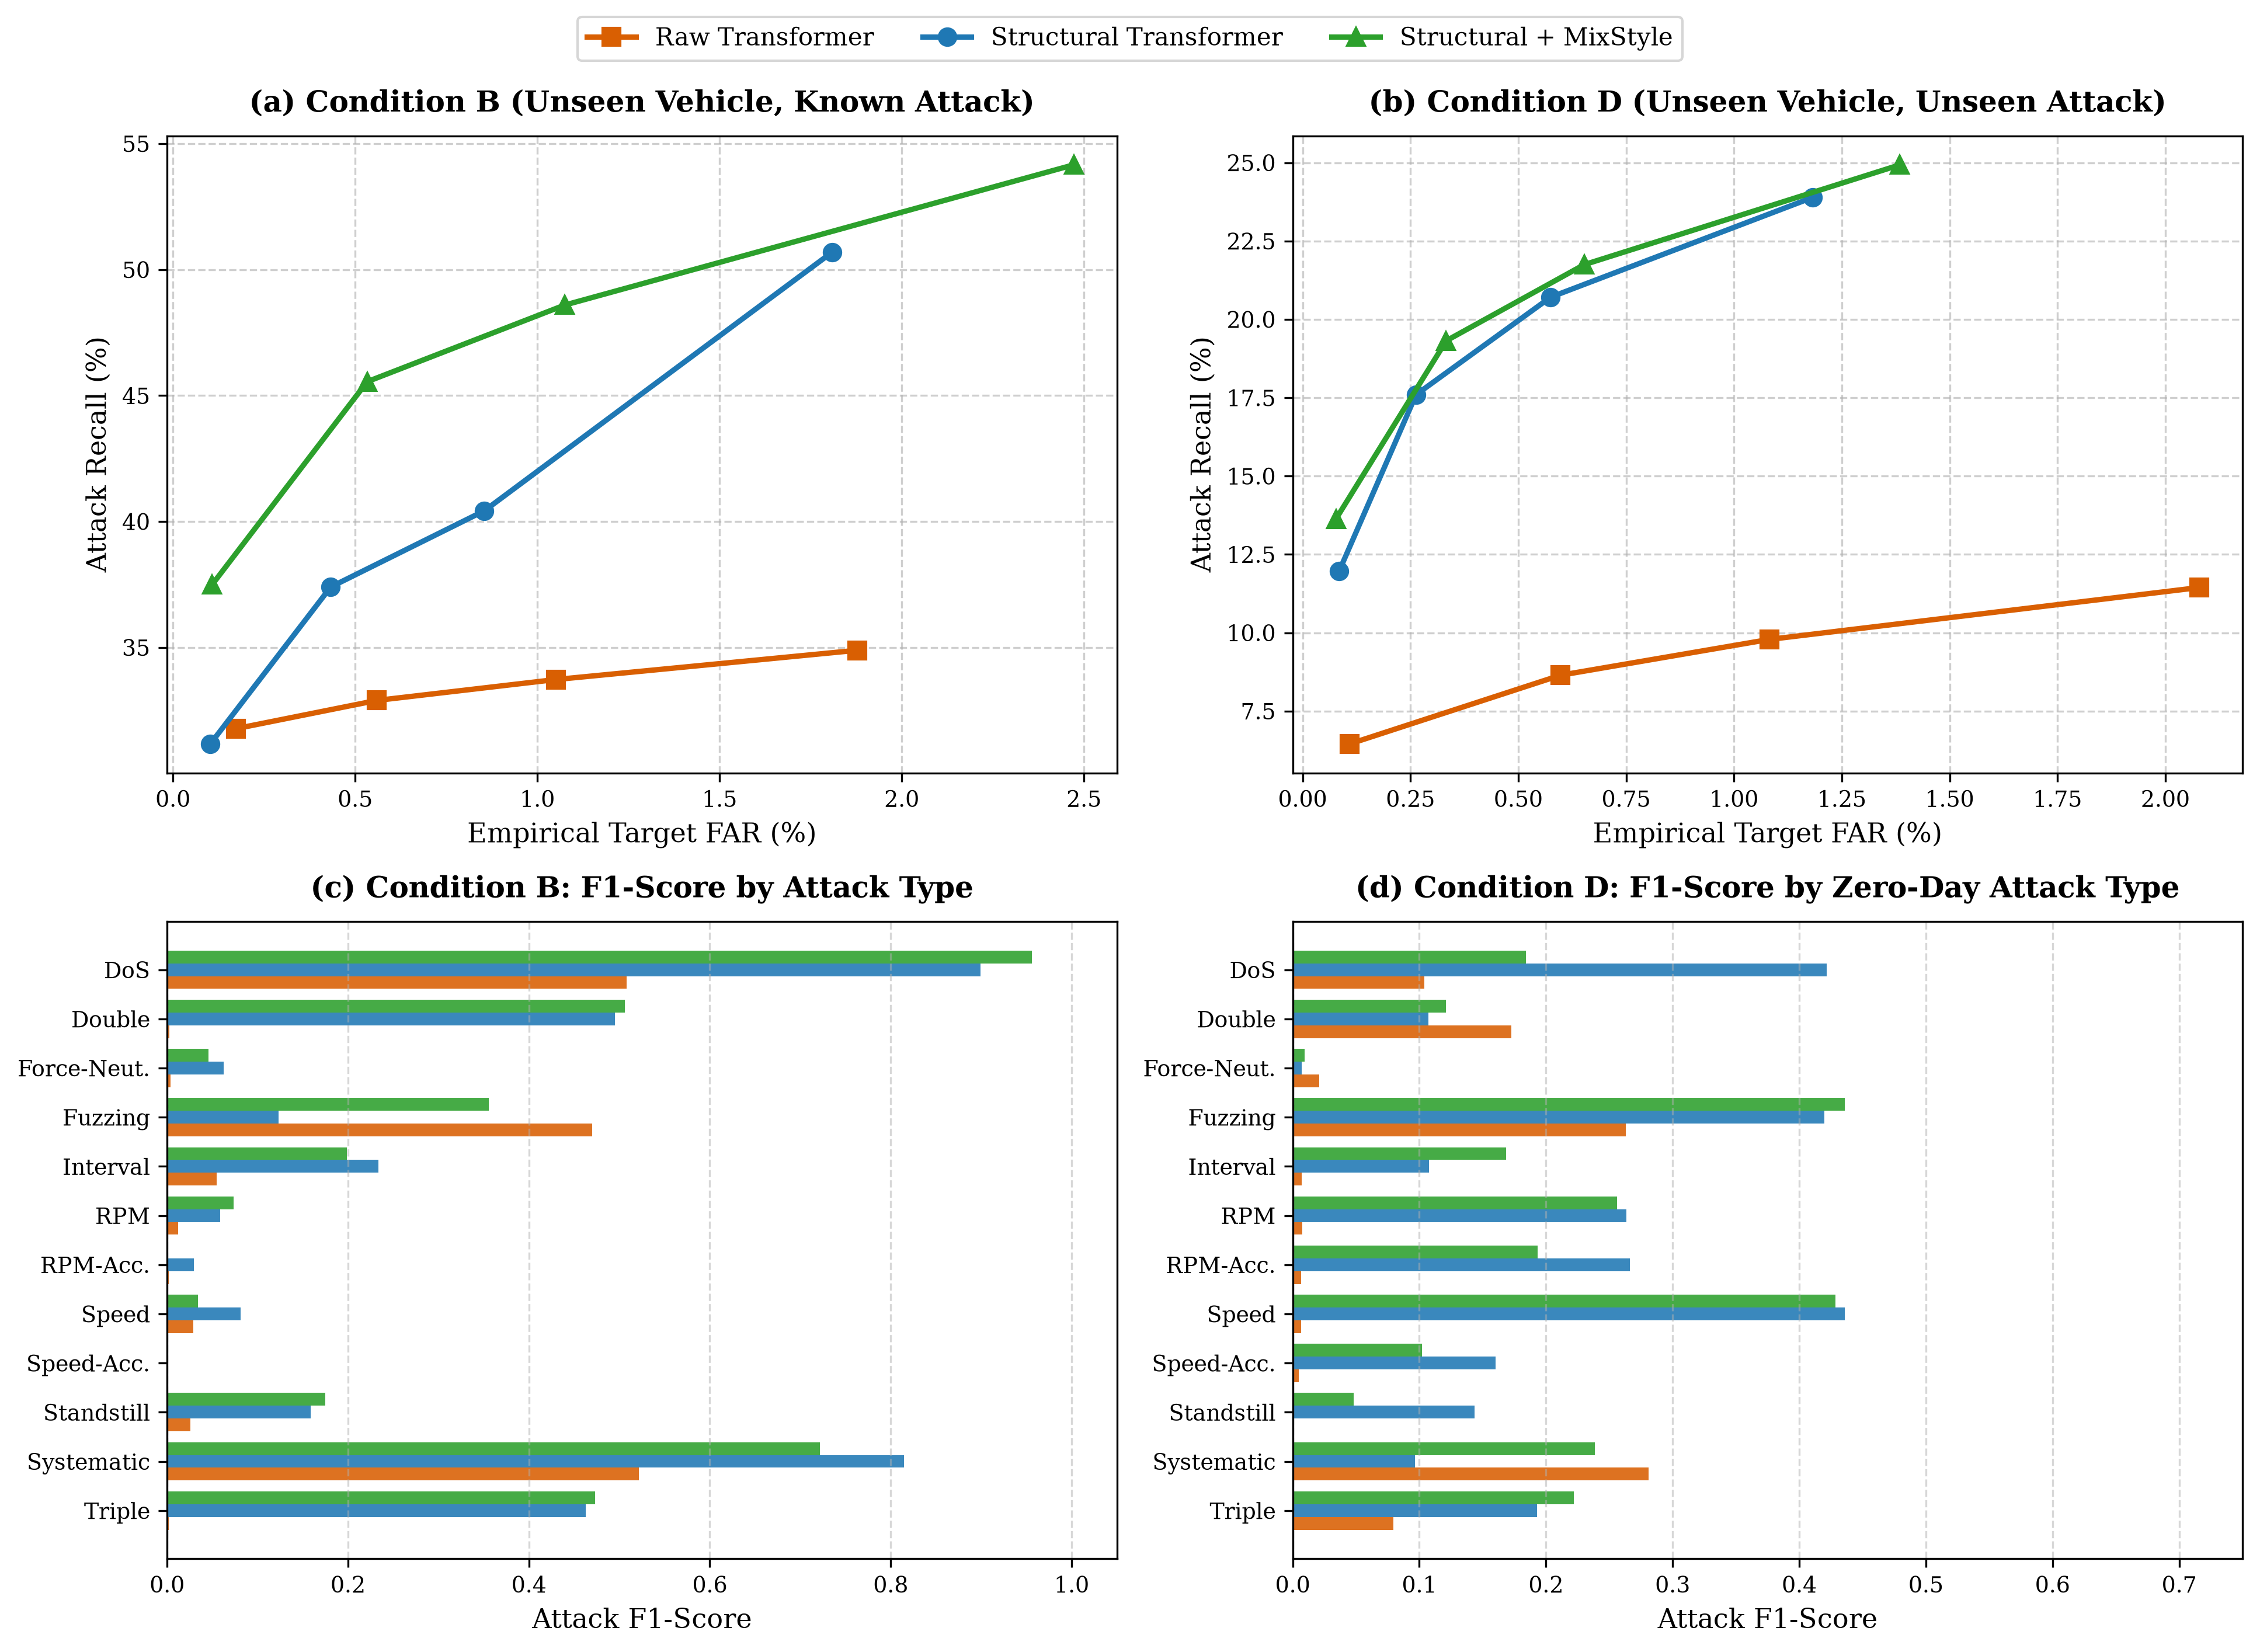
\includegraphics[width=0.80\textwidth]{figs/calibration_recovery_comparison.png}
\caption[Operational recovery evaluation via target benign warmup calibration]{Operational recovery under unsupervised target benign warmup calibration: (a)--(b) Recall versus empirical target FAR at $K=500$; (c)--(d) F1-score across individual attack types in Condition B and Condition D at $K=1000$ and $1.0\%$ FAR budget (complemented by the detailed comparison at $K \in \{200, 500, 1000\}$ in Table~\ref{tab:benign-calibration-summary}).}\label{fig:calibration-recovery}
\end{figure}

{\renewcommand{\arraystretch}{0.84}
\begin{table}[htbp]\centering\footnotesize\setlength{\tabcolsep}{4pt}
\caption[Operational recovery under benign warmup calibration across K=200, 500, 1000]{Operational recovery performance under unsupervised benign warmup calibration across $K \in \{200, 500, 1000\}$ (four-set mean, parenthesized values denote three-target-vehicle deduplicated mean)}\label{tab:benign-calibration-summary}
\begin{tabular}{P{0.9cm}P{0.9cm}P{1.7cm}P{2.9cm}P{2.2cm}P{1.4cm}P{1.2cm}P{1.2cm}}
\toprule
Cond & $K$ & Budget & Pipeline & Recall (3-veh) & FAR (\%) & AP & F1\\\midrule
B & 200 & 1.0\% & Structural + MixStyle & 0.4734 (0.4949) & 1.2163 & 0.5832 & 0.5344\\
B & 500 & 0.1\% & Raw & 0.3177 (0.3743) & 0.1727 & 0.3803 & 0.3810\\
B & 500 & 0.1\% & Structural & 0.3117 (0.3460) & 0.1024 & 0.5607 & 0.4227\\
B & 500 & 0.1\% & Structural + MixStyle & \textbf{0.3749} (0.3999) & 0.1077 & \textbf{0.5845} & \textbf{0.4955}\\
B & 500 & 1.0\% & Raw & 0.3373 (0.3922) & 1.0509 & 0.3803 & 0.3788\\
B & 500 & 1.0\% & Structural & 0.4042 (0.4303) & 0.8545 & 0.5607 & 0.4748\\
B & 500 & 1.0\% & Structural + MixStyle & \textbf{0.4859} (0.5042) & 1.0752 & \textbf{0.5845} & \textbf{0.5450}\\
B & 1000 & 0.1\% & Structural + MixStyle & 0.4002 (0.4246) & 0.0999 & 0.5864 & 0.5150\\
B & 1000 & 1.0\% & Structural + MixStyle & \textbf{0.5141} (0.5218) & 0.9710 & \textbf{0.5864} & \textbf{0.5697}\\
\midrule
D & 200 & 1.0\% & Structural + MixStyle & 0.2124 (0.2283) & 0.5086 & 0.3680 & 0.2863\\
D & 500 & 0.1\% & Raw & 0.0645 (0.0834) & 0.1087 & 0.1692 & 0.1018\\
D & 500 & 0.1\% & Structural & 0.1196 (0.1403) & 0.0845 & 0.3411 & 0.1793\\
D & 500 & 0.1\% & Structural + MixStyle & \textbf{0.1363} (0.1611) & 0.0772 & \textbf{0.3702} & \textbf{0.2026}\\
D & 500 & 1.0\% & Raw & 0.0979 (0.1257) & 1.0818 & 0.1692 & 0.1195\\
D & 500 & 1.0\% & Structural & 0.2071 (0.2255) & 0.5750 & 0.3411 & 0.2728\\
D & 500 & 1.0\% & Structural + MixStyle & \textbf{0.2175} (0.2340) & 0.6529 & \textbf{0.3702} & \textbf{0.2852}\\
D & 1000 & 1.0\% & Structural + MixStyle & 0.2211 (0.2375) & 0.7078 & 0.3728 & 0.2869\\
\bottomrule\end{tabular}
\end{table}}

{\renewcommand{\arraystretch}{0.84}
\begin{table}[htbp]\centering\footnotesize\setlength{\tabcolsep}{4pt}
\caption[Benign calibration comparison for baselines and sliding m-of-n event filtering]{Comparison of unsupervised benign warmup calibration across baseline models and the impact of sliding $m$-of-$n$ event filtering ($K=500$, $1.0\%$ FAR budget)}\label{tab:cal-baselines-mofn}
\begin{tabular}{P{4.2cm}P{0.9cm}P{1.6cm}P{1.6cm}P{1.6cm}P{1.65cm}P{1.3cm}}
\toprule
Method / Rule & Cond & Recall & FAR (\%) & F1 & Precision & AP\\\midrule
CANBERT+ adapted (Calib. $K=500$) & B & 0.2428 & 20.5601 & 0.1078 & -- & 0.0997\\
CANLP-char-DNN adapted (Calib. $K=500$) & B & 0.6578 & 68.2462 & 0.0794 & -- & 0.0564\\
Raw TF (1-of-1) & B & 0.3373 & 1.0509 & 0.3788 & -- & 0.3803\\
Structural TF (1-of-1) & B & 0.4042 & 0.8545 & 0.4748 & 0.6846 & 0.5607\\
Structural + MixStyle (1-of-1) & B & 0.4859 & 1.0752 & 0.5450 & 0.6603 & 0.5845\\
Structural + MixStyle (2-of-3) & B & 0.4911 & \textbf{0.2234} & 0.5903 & 0.8496 & --\\
Structural + MixStyle (2-of-5) & B & \textbf{0.5351} & 0.5491 & \textbf{0.6141} & 0.7704 & --\\
Structural + MixStyle (3-of-5) & B & 0.4926 & \textbf{0.1387} & 0.5947 & \textbf{0.9131} & --\\
\midrule
Structural + MixStyle (1-of-1) & D & 0.2175 & 0.6529 & 0.2852 & 0.4857 & 0.3702\\
Structural + MixStyle (2-of-3) & D & 0.1995 & \textbf{0.1160} & 0.2820 & 0.5738 & --\\
Structural + MixStyle (3-of-5) & D & 0.1919 & \textbf{0.0575} & 0.2747 & \textbf{0.6091} & --\\
\bottomrule\end{tabular}
\end{table}}

From Table~\ref{tab:benign-calibration-summary}, Table~\ref{tab:cal-baselines-mofn}, and Figure~\ref{fig:calibration-recovery}, five quantitative conclusions emerge:
\begin{enumerate}
    \item \textbf{Operational recovery and tail quantile resolution:} At $K=500, \alpha=1.0\%$ in Condition B, \code{CANBERT+} (FAR $20.56\%$) and \code{CANLP-char-DNN} (FAR $68.25\%$) still violate the budget, whereas Structural reaches $40.42\%$ recall ($\text{FAR}=0.8545\%$) and Structural+MixStyle reaches $48.59\%$ (3-vehicle mean $50.42\%$, $\text{FAR}=1.0752\%$). At $K=500, \alpha=0.1\%$, $K\alpha = 0.5 < 1$ inflates tail variance compared with $K=1000$ ($K\alpha = 1$). Per-set breakdown (Table~\ref{tab:cal-k-per-set}, Appendix~\ref{app:sensitivity}) shows strong recovery in Set~1 ($88.44\%$) and Set~3 ($53.14\%$) versus modest recall in Set~4 ($19.74\%$).
    \item \textbf{Hourly false-alarm suppression via sliding $m$-of-$n$ filtering:} At bus rates of $1{,}000$--$2{,}000$ frames/s ($56{,}250$--$112{,}500$ windows/hour), \code{2-of-3} cuts Condition B FAR nearly $5\times$ to $0.2234\%$ (Precision $0.8496$, Recall $49.11\%$), while \code{3-of-5} lowers Condition B FAR to $0.1387\%$ (Precision $0.9131$) and Condition D FAR to $0.0575\%$ (without claiming frame-level localization).
    \item \textbf{Warmup contamination sensitivity:} Injecting $1\%, 2\%, 5\%$ attack windows into the $K=500$ prefix of Structural+MixStyle drops Condition B recall ($\alpha=1.0\%$) from $48.59\%$ to $47.24\%$, $44.95\%$, and $32.85\%$ (at $\alpha=0.1\%$, $1\%$ poisoning halves recall from $37.49\%$ to $16.06\%$, and $5\%$ drops it to $5.33\%$).
    \item \textbf{Granular per-attack breakdown:} In Condition B ($K=500, 1.0\%$, Figure~\ref{fig:calibration-recovery}c), Structural+MixStyle achieves $92.42\%$ recall on DoS (F1 $0.9438$ vs Raw $0.5040$) and $72.35\%$ on Systematic (F1 $0.7177$), whereas \code{force-neutral} ($0.38\%$) and \code{speed} ($7.31\%$) remain low; in Condition D (Figure~\ref{fig:calibration-recovery}d), \code{speed} reaches $40.13\%$ (Raw $1.03\%$) and \code{fuzzing} reaches $39.71\%$.
    \item \textbf{External validation ($K=500, \alpha=0.1\%$, 3 seeds):} \textit{Opel\_Astra\_DoS} suppresses FAR to $0.271\% \pm 0.266\%$ (Structural) and $0.167\% \pm 0.079\%$ (MixStyle) at $1.0000$ recall; \textit{Renault\_Clio\_DoS} retains $0.9984$ recall with $0.0000\%$ FAR (Raw $0.0508\%$ benign); \textit{\mbox{CICIoV2024}} escapes its $100\%$ FAR collapse ($0.047\%$ and $0.086\%$) though seed variance is extreme (Structural recall $0.3336 \pm 0.5242$, AP $0.9172 \pm 0.0711$; MixStyle recall $0.0001 \pm 0.0002$ at $0.1\%$ and $0.3229 \pm 0.5593$ at $1.0\%$); and \textit{CAN\_MIRGU} maintains $0.087\%\text{--}0.094\%$ FAR ($1.135\%\text{--}1.236\%$ benign) at low recall $0.0065\text{--}0.0072$ ($0.0275\text{--}0.0308$ at $1.0\%$).
\end{enumerate}

\noindent\textbf{Target-only benchmarks without source training ($K=500$):} On target-only \code{IsolationForest} and \texttt{Split-Mahalanobis} controls (Section~\ref{subsec:target-only-k500}, Table~\ref{tab:target-only-k500}, Appendix~\ref{app:sensitivity}), \texttt{Split-Mahalanobis St60} (250/250) achieves high AP ($0.7048$ in B; $0.7605$ in D), yet estimating a 60D covariance matrix on 250 autocorrelated windows causes empirical FAR to drift to $1.225\%\text{--}7.564\%$ ($5\times\text{--}15\times$ over budget), whereas the frozen source Transformer calibrating a single scalar 1D threshold holds empirical FAR tightly near budget ($0.102\%\text{--}1.075\%$).

\subsection{Multi-source LOVO training with conditional adversarial classification}\label{sec:multisource-lovo}
To evaluate whether combining multiple source vehicles with conditional domain-adversarial alignment (LOVO-cAdv DANN, formulated in Section~\ref{subsec:method-lovo}) enables zero-shot detection directly under source-calibrated thresholds on unseen vehicles, we conduct 48 Leave-One-Vehicle-Out training runs across all four CTT models (\textit{Forester, Impala, Silverado, Traverse}). Decision thresholds are selected exclusively on source validation sets (maximum observed source validation FAR $99.87/100\text{k}$). Probing samples are held out by recording-round groups with balanced vehicle $\times$ label cells (chance accuracy: vehicle $25\%$, attack $50\%$). The aggregate results (equally weighted across 4 target vehicles) and Figure~\ref{fig:multisource-lovo} are presented in Table~\ref{tab:multisource-lovo}.

\begin{figure}[htbp]
\centering
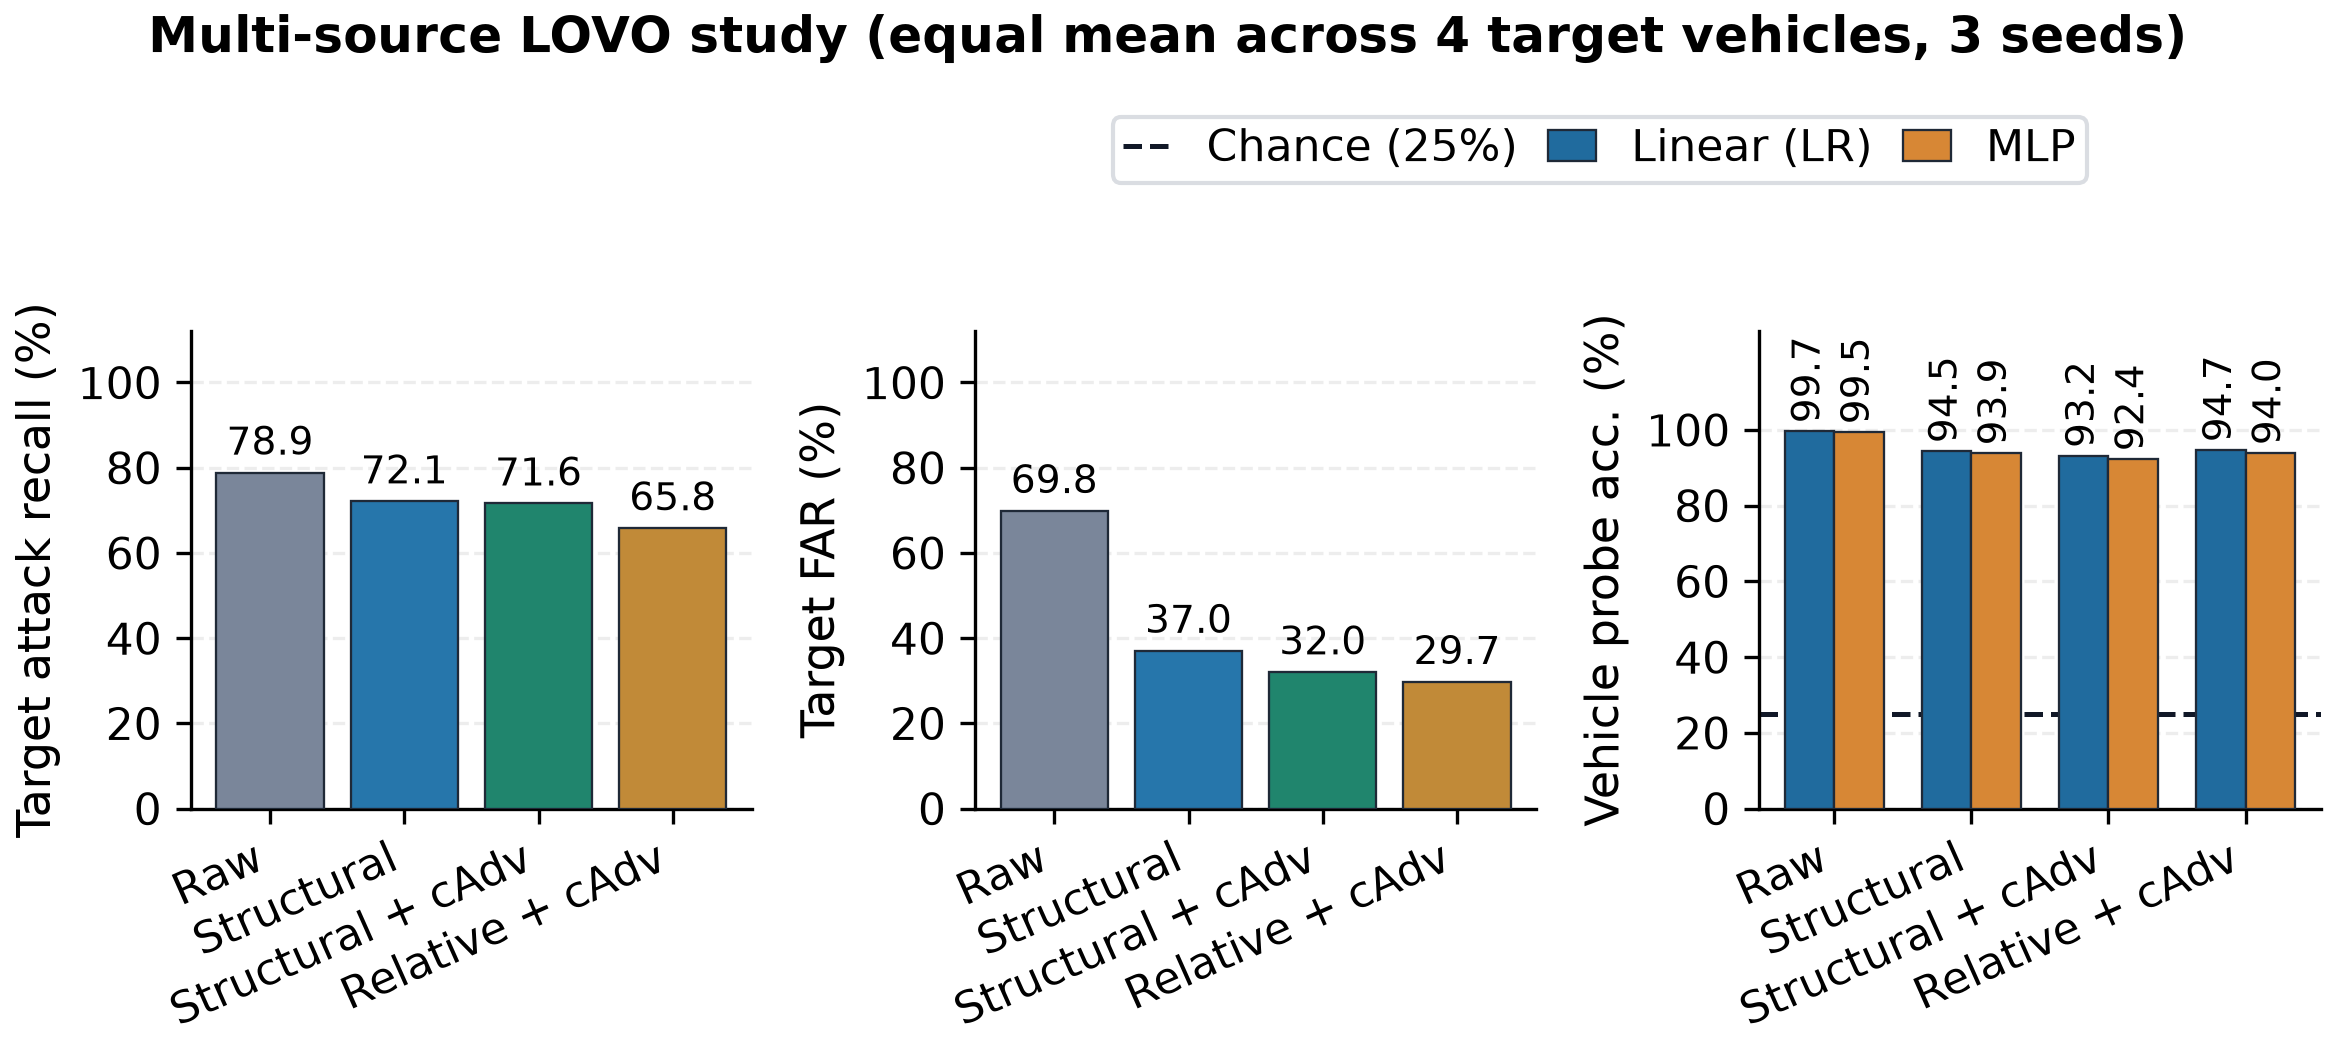
\includegraphics[width=0.80\textwidth]{figs/multisource_lovo_overview.png}
\caption[Multi-source LOVO performance and vehicle-identity probing]{Multi-source LOVO performance (equal mean across 4 held-out target vehicles $\times$ 3 seeds) under source validation thresholds alongside linear/MLP vehicle probing accuracy (chance level: $25\%$).}\label{fig:multisource-lovo}
\end{figure}

{\renewcommand{\arraystretch}{0.85}
\begin{table}[htbp]\centering\footnotesize\setlength{\tabcolsep}{4pt}
\caption[Multi-source LOVO results with conditional domain-adversarial alignment]{Multi-source Leave-One-Vehicle-Out (LOVO) results with conditional domain-adversarial alignment (48 training runs, equal weighting across four target vehicles, source-only threshold selection)}\label{tab:multisource-lovo}
\begin{tabular}{P{2.8cm}P{1.4cm}P{2.6cm}P{1.2cm}P{1.2cm}P{1.8cm}P{1.8cm}}
\toprule
Method & Recall & FAR /100k (\%) & AP & F1 & Vehicle Probe (LR/MLP) & Attack Probe (LR) \\ \midrule
Raw & 0.7885 & 69835.3 (69.84\%) & 0.2196 & 0.2182 & 99.74\% / 99.47\% & 61.51\% \\
Structural & \textbf{0.7211} & 37022.5 (37.02\%) & \textbf{0.6020} & 0.4073 & 94.49\% / 93.89\% & 80.47\% \\
Structural + cAdv & 0.7161 & 31974.5 (31.97\%) & 0.5970 & \textbf{0.4254} & \textbf{93.22\%} / \textbf{92.36\%} & \textbf{81.11\%} \\
Relative + cAdv & 0.6579 & \textbf{29721.1} (29.72\%) & 0.5764 & 0.4148 & 94.74\% / 93.96\% & 79.94\% \\
\midrule
\multicolumn{7}{P{13.6cm}}{\footnotesize \textit{Note:} Boldface highlights the best performance among the proposed structure-based models (Raw attains Recall 0.7885 but degenerates with FAR reaching 69.84\% and AP only 0.2196). Lower vehicle probe accuracy indicates reduced vehicle-identity leakage.}\\
\bottomrule
\end{tabular}
\end{table}}

The metrics in Table~\ref{tab:multisource-lovo} provide critical negative evidence regarding pure zero-shot multi-source transfer: although training across three diverse source vehicles boosts the AP of Structural to $0.6020$ (versus Raw $0.2196$) and adding conditional domain-adversarial alignment (\code{cAdv}) modestly reduces frozen source threshold FAR from $37.02\%$ to $31.97\%$ (increasing F1 to $0.4254$), target FAR remains unacceptably high and volatile across makes. Per-target breakdown of \code{structural\_cadv} reveals that \textit{Traverse} achieves FAR $0.058\%$ (recall $51.35\%$, AP $0.6193$) and \textit{Impala} achieves FAR $0.473\%$ (recall $54.26\%$, AP $0.6314$), but \textit{Silverado} explodes to FAR $47.46\%$ (recall $85.46\%$, AP $0.6485$) and \textit{Forester} to $79.91\%$ (recall $95.40\%$, AP $0.4890$). Concurrently, linear vehicle decoding on the frozen embedding of \code{structural\_cadv} remains at $93.22\%$ (LR) and $92.36\%$ (MLP). This empirical finding confirms that even under multi-source DANN training, the encoder retains substantial vehicle-discriminative information and cannot rely on a static source threshold to operate effectively on unobserved vehicles.

\subsection[Benign Covariance Whitening, LEACE/INLP8, and Energy Evaluation]{Benign-target covariance whitening combined with linear concept erasure (LEACE/INLP8) and energy scoring}\label{sec:benign-invariant}
Following the failure of static source thresholds in Section~\ref{sec:multisource-lovo}, we evaluate the geometric feature purification framework across 96 post-hoc pipelines (12 frozen Structural LOVO encoders $\times$ 8 methodological branches) alongside the Mahalanobis energy score (\code{white\_energy}) as designed in Section~\ref{subsec:method-whitening}. Each target vehicle reserves an authentic benign capture (54,231 windows strictly excluded from evaluation, with an additional 740 exact W64 duplicates removed via SHA-256 \code{content\_disjoint} check). Transformations \code{LEACE}, \code{INLP8} (truncated at 8 dimensions), \code{PCA8}, and logistic regression (LR) heads are fitted strictly on the three source vehicles. Results are summarized in Table~\ref{tab:benign-invariant-main} and Figure~\ref{fig:benign-invariant}.

\begin{figure}[htbp]
\centering
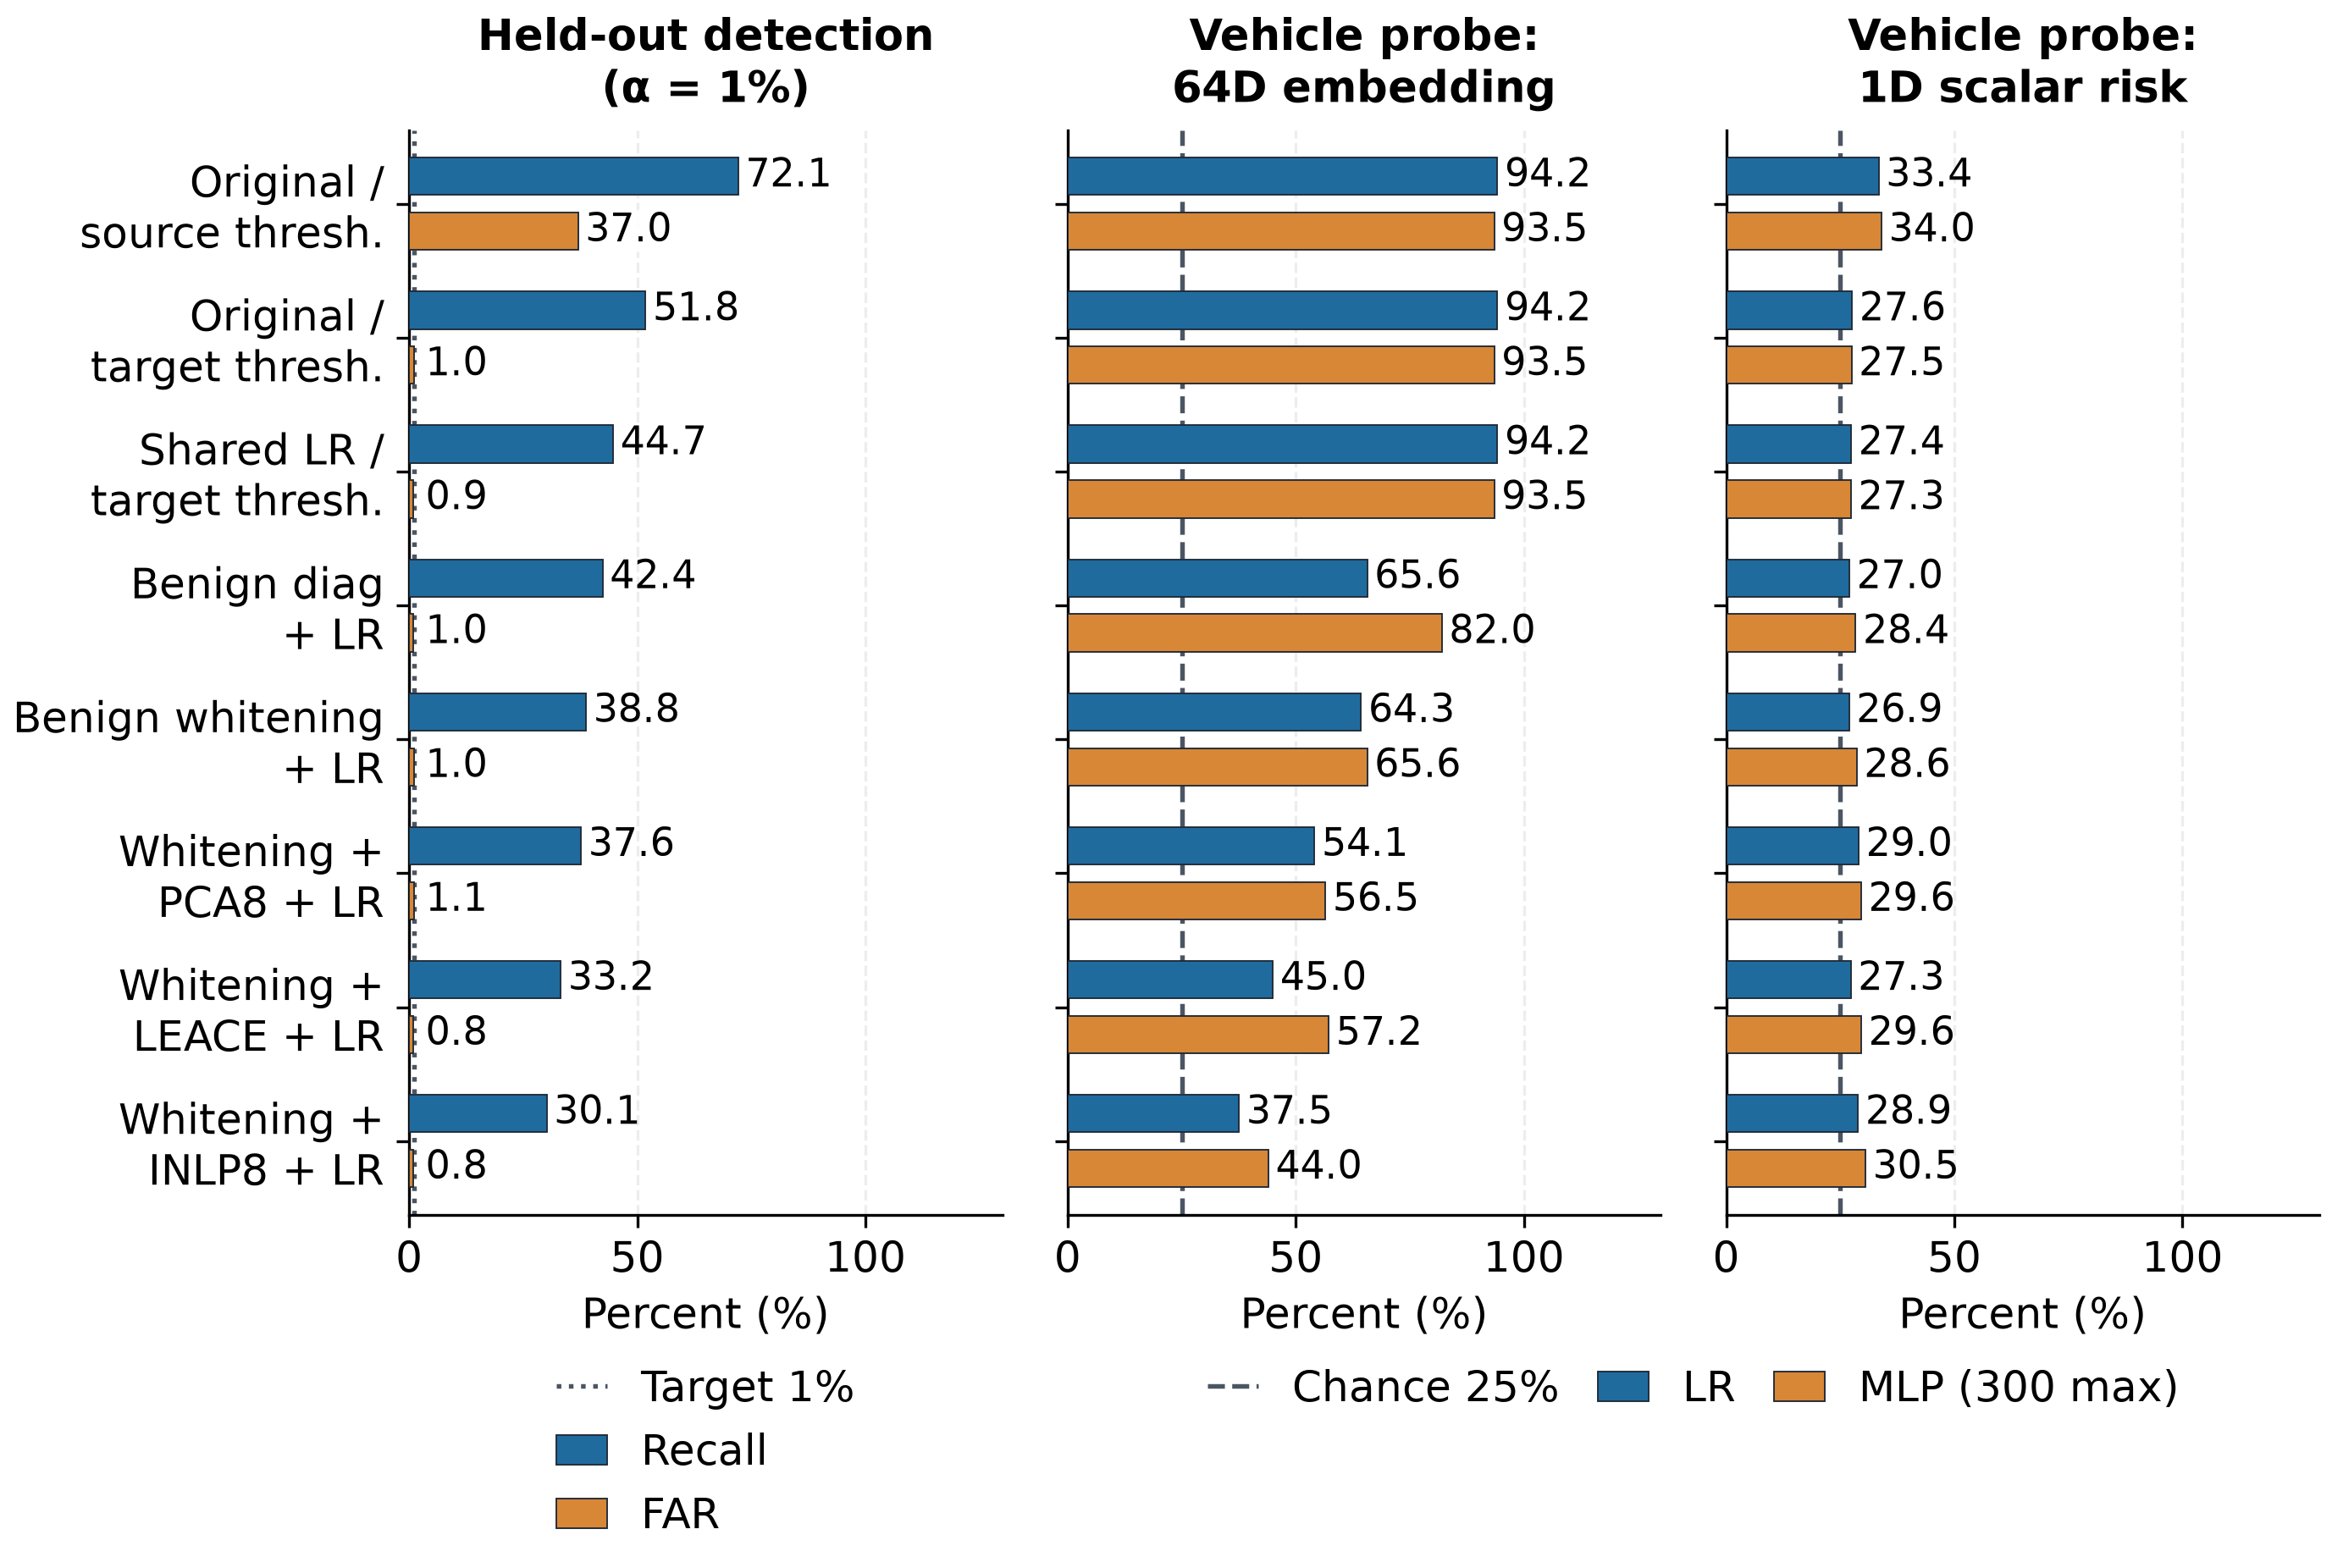
\includegraphics[width=0.80\textwidth]{figs/benign_invariant_overview.png}
\caption[Dual intrusion detection and probing after whitening and concept erasure]{Dual evaluation of intrusion detection ($\alpha=1\%$, \code{content\_disjoint}), 4-vehicle decoding on 64D embeddings, and vehicle probing on 1D anomaly risk scores (chance level: $25\%$).}\label{fig:benign-invariant}
\end{figure}

{\renewcommand{\arraystretch}{0.84}
\begin{table}[htbp]\centering\footnotesize\setlength{\tabcolsep}{3.5pt}
\caption[Comparison of benign-target whitening with linear concept erasure and energy scoring]{Comparison of benign-target covariance whitening combined with linear concept erasure (LEACE/INLP8) and Mahalanobis energy scoring \code{white\_energy} ($\alpha=1.0\%$ normalized budget, \code{content\_disjoint})}\label{tab:benign-invariant-main}
\begin{tabular}{P{2.85cm}P{1.1cm}P{1.3cm}P{1.1cm}P{1.1cm}P{1.85cm}P{1.6cm}P{1.5cm}}
\toprule
Method & Recall & FAR (\%) & F1 & AP & 64D Probe (LR / MLP300) & MLP 1500-iter & 1D Risk (LR) \\ \midrule
Original / source thresh. & 0.7211 & 37.001 & 0.4096 & 0.6042 & 94.18\% / 93.46\% & 93.46\% & 33.40\% \\
Original / target thresh. & \textbf{0.5180} & 1.009 & \textbf{0.6032} & 0.6042 & 94.18\% / 93.46\% & -- & 27.58\% \\
Shared LR / target thresh. & 0.4469 & 0.889 & 0.5362 & 0.5544 & 94.18\% / 93.46\% & -- & 27.38\% \\
Benign diag + LR & 0.4239 & 0.990 & 0.5152 & 0.5243 & 65.63\% / 81.99\% & -- & 26.99\% \\
Benign whitening + LR & 0.3876 & 1.036 & 0.4705 & 0.4852 & 64.29\% / 65.63\% & -- & 26.92\% \\
Whitening + PCA8 + LR & 0.3765 & 1.100 & 0.4361 & 0.4603 & 54.08\% / 56.48\% & 53.68\% & 29.03\% \\
Whitening + LEACE + LR & 0.3321 & \textbf{0.844} & 0.4065 & 0.4242 & 44.96\% / 57.19\% & 57.17\% & \textbf{27.30\%} \\
Whitening + INLP8 + LR & 0.3013 & \textbf{0.844} & 0.3750 & 0.3715 & \textbf{37.53\%} / \textbf{43.97\%} & \textbf{42.01\%} & 28.90\% \\
\midrule
\code{white\_energy} ($\alpha=0.1\%$) & 0.4606 & \textbf{0.297} & \textbf{0.5918} & \textbf{0.6172} & -- & -- & -- \\
\code{white\_energy} ($\alpha=1.0\%$) & 0.6008 & 3.831 & 0.5323 & \textbf{0.6172} & -- & -- & -- \\
\midrule
\multicolumn{8}{P{13.8cm}}{\footnotesize \textit{Note:} Boldface in the upper block indicates the best performance among supervised binary classifiers at $\alpha=1.0\%$; the lower block reports the unsupervised Mahalanobis energy score \code{white\_energy} (achieving Recall 0.6008 at $\alpha=1.0\%$ and FAR 0.297\% at $\alpha=0.1\%$).}\\
\bottomrule
\end{tabular}
\end{table}}

Three primary methodological insights emerge from Table~\ref{tab:benign-invariant-main} and Figure~\ref{fig:benign-invariant}:
\begin{enumerate}
    \item \textbf{Decoupling 1D risk score erasure from 64D representation erasure:} Even without whitening or concept erasure, simply projecting the embedding onto a 1D scalar risk score and applying a threshold collapses vehicle probing from $33.40\%$ to $27.30\%\text{--}28.90\%$ (near the random baseline of $25\%$), whereas the underlying 64D representation retains $94.18\%$ vehicle decoding. Asserting vehicle independence based solely on 1D anomaly score probing is a measurement artifact.
    \item \textbf{Trade-offs in linear concept erasure and residual non-linear leakage:} Combining target benign whitening with source-fitted LEACE or INLP8 substantially suppresses 64D linear vehicle probing from $94.18\%$ down to $44.96\%$ (LEACE) and $37.53\%$ (INLP8), far exceeding simple whitening ($64.29\%$) or PCA8 compression ($54.08\%$), while maintaining attack separability at $79.05\%\text{--}81.44\%$. However, this suppression penalizes detection recall, which drops from $51.80\%$ (\textit{Original / target thresh.}, $\text{AP}=0.6042$) to $33.21\%$ (LEACE, $\text{AP}=0.4242$) and $30.13\%$ (INLP8, $\text{AP}=0.3715$), especially on challenging vehicles (\textit{Silverado} and \textit{Forester}). Crucially, non-linear stress testing via 1,500-iteration MLP probing recovers $57.17\%$ (LEACE) and $42.01\%$ (INLP8) accuracy, proving that linear nullspace projection leaves non-linear vehicle identity intact.
    \item \textbf{Efficacy of whitened Mahalanobis energy scoring (\code{white\_energy}):} Instead of projecting through linear classifiers, measuring raw Mahalanobis energy distance directly on target-whitened 64D embeddings achieves the highest AP across all evaluated paradigms ($\text{AP} = 0.6172$). At $\alpha=0.1\%$, it delivers recall $46.06\%$, FAR $0.297\%$ ($297.3/100\text{k}$), and F1 $0.5918$ (Impala $59.09\%$, Silverado $53.97\%$, Traverse $52.33\%$, Forester $18.85\%$). However, at $\alpha=1.0\%$, empirical FAR slips to $3.83\%$ because automotive CAN temporal autocorrelation violates the i.i.d.\ assumption under 1,000-window calibration samples.
\end{enumerate}

\section{Host processing cost and threats to validity}
\subsection{Processing cost on the experimental host}\label{sec:runtime}
Table~\ref{tab:runtime-decomp} isolates three-component per-window processing latency on CPU and GPU (\code{batch=1}, 20 warmup + 900 windows of \code{accessory-2.csv}); the two aggregate I/O-and-dual-extraction tables (Table~\ref{tab:extension-runtime}, $6.176\text{ ms}$, and Table~\ref{tab:mixstyle-runtime}, $4.001\text{ ms}$) are archived in Section~\ref{subsec:app-runtime-audit}, Appendix~\ref{app:sensitivity}.

{\renewcommand{\arraystretch}{0.86}
\begin{table}[htbp]\centering\footnotesize
\caption{Three-component per-window processing latency decomposition at $W=64$ on CPU and GPU ($N=900$, \code{batch=1}, in ms)}\label{tab:runtime-decomp}
\begin{tabular}{P{1.6cm}P{2.5cm}P{2.5cm}P{2.5cm}P{2.8cm}}
\toprule
Device & CSV Read (Median) & Dual 28D+30D Extraction (Median) & Structural Inference (Median) & Total E2E Structural (Median / P95) \\ \midrule
CPU & 1.083 & 3.036 & 0.731 & 4.830 / 6.231 \\
CUDA & 0.932 & 2.285 & 1.150 & 4.402 / 5.291 \\
\bottomrule
\end{tabular}
\end{table}}

Pure inference latency of \code{Structural Transformer} on CPU is only $0.731\text{ ms}$ (comparable to Raw $0.768\text{ ms}$ and faster than CUDA $1.150\text{ ms}$ at \code{batch=1}), whereas CSV reading ($1.083\text{ ms}$) and dual extraction ($3.036\text{ ms}$) dominate end-to-end benchmark latency; on a $500\,\text{kbps}$ bus ($1{,}000\text{--}2{,}000$~frames/s), window buffering adds $32\text{--}64\text{ ms}$ for $W=64$ (total $\approx 37\text{--}70\text{ ms}$). The static complexity audit (Section~\ref{subsec:complexity-audit}, Table~\ref{tab:model-complexity-audit}, Appendix~\ref{app:sensitivity}) confirms that Structural adds only $128$ parameters ($75{,}298$ vs $75{,}170$, $+0.17\%$), $8{,}192$ MACs ($+0.15\%$), and $130.00\text{ KiB}$ of history state RAM $H_k$, remaining $720\times$ smaller in parameters and $5{,}075\times$ lighter in MACs than \code{CANBERT+} ($54.25\text{M}$ parameters, $206.94\text{ MiB}$, $27.24\text{G}$ MACs). Real-time ECU deployment is not certified by desktop timings.

\subsection{Threats to validity}\label{sec:threats-to-validity}
Synthesizing all experimental phases from the primary matrix to the post-hoc extensions, we identify five primary threats to validity:
\begin{enumerate}
    \item \textbf{Construct validity and target vehicle replication:} The four CTT benchmark sets utilize only 4 physical vehicles and 3 distinct target makes (Subaru Forester is duplicated in Set 2 and Set 3), and partitions by recording-round suffix lack physical metadata verifying independent driving sessions. Window labelling ($W=64$) requires only one positive frame and does not evaluate frame localization or pre-harm latency; comparators (\code{CANBERT+}, \code{CANLP}, \code{AssocRules}) differ in supervision and parameter scale, and \code{AssocRules} degenerates to $1.0000000000000002$ under strict budgets.
    \item \textbf{Tail quantile stability and unlabelled calibration:} Selecting a $0.1\%$ FAR threshold from source validation on uncalibrated cross-entropy logits induces severe drift (e.g., Structural Set 1 Seed 42 or CANBERT+ collapse). In the benign warmup regime ($K=500$, $\alpha=0.1\%$), the product $K\alpha = 0.5 < 1$ constrains quantile resolution and remains sensitive to $1\%\text{--}5\%$ adversarial contamination during ignition; similarly, the covariance whitening protocol in Section~\ref{sec:benign-invariant} requires 2,000 windows distributed across an entire benign file rather than an online stream and does not guarantee distribution-free tail bounds under autocorrelated CAN traffic.
    \item \textbf{Linear probing bounds and optimization warnings:} Logistic regression and MLP probes exhibited convergence/optimization warnings in certain configurations (98/576 cells in LOVO, 133 cells in whitening studies, including baseline controls); furthermore, suppressing 1D risk score or linear embedding probes does not establish non-linear invariance, as 1,500-iteration MLPs retain $42.01\%\text{--}57.17\%$ vehicle decoding.
    \item \textbf{Post-hoc exploration and physical chronology:} Ablation, MixStyle, calibration, LOVO, and benign whitening rounds were designed after inspecting initial 4-set outcomes; the content-only evaluation preserves CSV row order based on audit verification that all timestamp reversals are $\le 7.895\,\text{ms}$, but cannot substitute for validation on datasets with verified physical chronology and completely unobserved vehicle makes.
    \item \textbf{Disparity between desktop hosts and embedded ECUs:} Runtime benchmarks in Section~\ref{sec:runtime} were obtained on desktop CPU/GPU hardware with \code{batch=1}; execution times do not capture constrained memory, bus contention, or hard deadline constraints of microcontrollers in physical ECUs, and all configurations incur an inherent $32\text{--}64\,\text{ms}$ buffering latency to assemble $W=64$ frames.
\end{enumerate}

\section{Chapter summary}
This chapter presented controlled empirical evaluations spanning the 60-unit primary matrix, component ablations, window-length sensitivity, diagnostic linear probes, 57 external captures, adaptation regularizers, and unsupervised warmup calibration. Synthesized takeaways, limitations, and future directions are presented in \hyperref[chap:conclusion]{Conclusion and Future Work}.

\chap{Conclusion and future work}\label{chap:conclusion}
\sect{Summary of primary research findings}
Through rigorous controlled benchmarking across cross-vehicle transfer conditions and external automotive datasets, this thesis establishes the following core findings:

\textbf{Addressing RQ1 (Cross-vehicle transfer performance and threshold divergence):}
The investigational hypothesis that structural representation increases recall on unobserved target vehicles at window size $W=64$ under source-frozen thresholds ($\text{FAR} \le 100/100{,}000$) is not supported by the primary benchmark. At source thresholds, Structural achieves $73.83\%$ recall, approximately $11.59$ percentage points below Raw ($85.41\%$), while target false alarm rates remain elevated ($\text{FAR} = 52.46\%$). However, regarding threshold-independent anomaly ranking, Structural demonstrates clear superiority: Average Precision (AP) in Condition B rises from $0.3781$ to $0.5554$ (+17.74 percentage points paired difference; +17.73 percentage points difference of means over Raw and far outperforming CANBERT+ $0.0970$). The high target false alarm rate stems from an inter-vehicle static score distribution shift (\textit{threshold shift}). When paired with lightweight unsupervised benign warmup calibration ($K=500$, $\approx 16$\,s at $2{,}000$~frames/s or $\approx 32$\,s at $1{,}000$~frames/s upon ignition) in Section~\ref{sec:benign-calibration}, standalone Structural achieves $40.42\%$ recall at $0.8545\% < 1\%$ empirical FAR, while Structural+MixStyle reaches $48.59\%$ recall (empirical FAR $1.0752\%$ at a $1\%$ budget, reduced to $\le 0.22\%$ via $2\text{-of-}3$ or $3\text{-of-}5$ filtering).

\textbf{Addressing RQ2 (Component contribution tradeoffs within structural representation):}
Omitting raw identifier bits alone is insufficient to achieve effective transfer; removing CAN-IDs from the raw baseline degrades Condition B AP from $0.3781$ to $0.2200$. Individual feature components introduce decisive tradeoffs: local window statistics (frequency and first-seen rank within the window) are vital for ranking discrimination and anomaly sensitivity (ablating local statistics causes Condition B AP to collapse from $0.5554$ to $0.2894$). Conversely, removing absolute payload bytes and relying solely on payload dynamics ($\Delta$payload) prevents the model from overfitting to source attack signatures, dramatically boosting zero-day detection in Condition C (AP reaching $0.4730$ versus $0.2661$ for Raw).

\textbf{Addressing RQ3 (Vehicle-domain independence and feature entanglement):}
Diagnostic linear probing demonstrates that Structural inputs only slightly attenuate vehicle decoding accuracy from $0.9925$ to $0.9488$ ($4.37$ percentage points), remaining far above the $0.2500$ random-chance baseline. Root-cause feature probing reveals that message length syntax (\code{dlc\_and\_masks}: 9D DLC and valid-byte masks yielding $96.42\%$ plus 1D history flag $h_i$ yielding $27.46\%$, combining to $96.70\%$) and local traffic density ($75.65\%$) inherently encode manufacturer-specific bus topologies. Crucially, due to \textit{feature entanglement}, these vehicle-identifying structural channels also carry the primary signals for anomaly detection (attack-probe accuracy rising from $0.6419$ to $0.7669$). Consequently, manual feature ablation cannot eliminate vehicle identity without simultaneously crippling intrusion detection sensitivity. This proves that structural representations do not achieve complete vehicle independence, and cross-vehicle transfer necessitates domain adaptation techniques such as threshold calibration rather than relying on assumed absolute representation invariance.

\textbf{Addressing RQ4 (External generalization and practical deployment implications):}
Evaluation across 57 external captures indicates that practical cross-vehicle transfer depends intimately on syntactic message structure, identifier dictionaries, and label definition consistency. While the model achieves near-perfect detection on traffic-disrupting attacks ($99.84\%$ recall with $0.19\%$ source FAR and $0.00\%$ calibrated FAR on Renault Clio DoS, and $100\%$ recall with $0.17\%\text{--}0.27\%$ calibrated FAR on Opel Astra DoS), recall remains limited on CAN-MIRGU ($0.65\%\text{--}3.08\%$ post-calibration) and exhibits extreme initialization-seed variance on CICIoV2024 (Structural achieves mean recall $0.3336 \pm 0.5242$ with $\text{AP}=0.9172 \pm 0.0711$, whereas MixStyle yields $0.0001 \pm 0.0002$ at $0.1\%$ and $0.3229 \pm 0.5593$ at $1.0\%$; comparative analysis confirms that CICIoV2024 payload standard deviation is actually lower than CTT [$54.14$ vs $76.98$], attributing sensitivity to hexadecimal identifier format shifts rather than payload amplitude). These findings caution against extrapolating single-dataset benchmark scores to claims of universal IDS readiness, highlighting the necessity of dataset auditing and target baseline calibration.

\sect{Value and limitations}
The thesis supplies reproducible evaluation, representation controls and diagnostics separating ranking from decisions at source-selected thresholds. Consistent ID-renaming invariance is a tested narrow property, not vehicle independence. Negative outcomes bound the hypothesis and prevent isolated AP or recall from being interpreted as deployment success.

\subsection*{Findings from MixStyle, LOVO multi-source learning, and whitening--erasure}
MixStyle on single-source models increases Condition B recall relative to Structural but raises FAR ($64.54\%$) without reducing vehicle decoding ($0.9527$). Expanding to multi-source LOVO with conditional adversarial alignment (Section~\ref{sec:multisource-lovo}) confirms that even combining three source vehicles leaves static source thresholds with an average FAR of $31.97\%$ and vehicle probing of $93.22\%$. Combining target-benign covariance whitening across $2{,}000$ benign target windows with source-fitted LEACE/INLP8 (Section~\ref{sec:benign-invariant}) reduces 1D risk score vehicle probing to near-random levels ($27.30\%\text{--}28.90\%$) and 64D linear probing from $94.18\%$ to $37.53\%\text{--}44.96\%$, but trades off $18.6\text{--}21.7$ recall points and leaves non-linear vehicle identity intact (1,500-iteration MLP probing reaches $42.01\%\text{--}57.17\%$); meanwhile, whitened Mahalanobis energy achieves peak AP ($0.6172$, recall $46.06\%$, FAR $0.30\%$ at $\alpha=0.1\%$). Because this mechanism requires an unlabelled target benign stream for covariance estimation, a completely invariant zero-shot detector remains an open challenge.

\subsection*{Significance and constraints of unsupervised benign warmup calibration}
Experiments in Section~\ref{sec:benign-calibration} verify that performance degradation at source thresholds $\tau_{\text{src}}$ primarily reflects inter-make threshold shift. When supported by an unlabelled initial benign warmup budget ($K=500\text{--}1000$ windows, $\approx 16\text{--}32$\,s at ignition), Structural+MixStyle achieves Condition B recall $48.59\%\text{--}51.41\%$ (3-vehicle deduplicated: $50.42\%\text{--}52.18\%$) and Condition D recall $21.75\%\text{--}22.11\%$, while $2\text{-of-}3$ or $3\text{-of-}5$ event filtering suppresses empirical FAR to $0.14\%\text{--}0.22\%$. However, deployers must manage warmup contamination risks ($1\%\text{--}5\%$ adversarial injection degrades recall) and finite tail-quantile resolution when $K\alpha < 1$.

\sect{Future research}
Priorities are verified chronology and independent driving sessions (such as the ROAD dataset), vehicles excluded from development, and event-level detection latency. Extending benign warmup calibration to online test-time streaming adaptation offers a path for dynamic quantile tracking without interrupting packet processing. Embedded evaluation must measure resources, queues, ignition-cycle reset and LRU eviction policies for table $H_k$, buffering latency ($32\text{--}64\,\text{ms}$ for $W=64$), and hard deadlines on target automotive microcontrollers (ARM Cortex / Jetson Nano).

\appendix
\chapter{Reproducibility and evidence provenance}\label{app:reproducibility}
\section{Provenance and experimental scale}\label{sec:app-provenance}
The primary matrix has 60 IDS units (4 sets $\times$ 3 seeds $\times$ 5 methods). Post-hoc explorations comprise 144 new fits and 24 baseline references across window sizes ($W \in \{32, 64, 128\}$), 12 Structural+MixStyle fits, grid calibration ($K \in \{200, 500, 1000\}$), 48 multi-source LOVO fits with conditional DANN, 96 benign whitening and LEACE/INLP8 pipelines, and 120 extended verification runs (48 monotonic Timed/Content controls, 48 frame-equated windows, 24 reservoir sampling variance runs). Fifty-seven external captures do not represent 57 independent driving sessions. Complete result tables, bootstrap distributions, source score distributions, integrity hashes, and input-exclusion records are systematically archived in the study's reproducibility record.

\subsection{Integrity Hashes and Reference Implementation Commits}\label{subsec:app-hashes}
To guarantee full bit-to-bit auditability and independent reproducibility, the cache manifest SHA-256 hash and competitor source commits are pinned as follows:
\begin{itemize}
    \item \textbf{CTT Cache Manifest SHA-256:} \texttt{\seqsplit{03a6bbf16efb4f583ca5566025c8bdc3cc0b65a7138a0a29f652505b2c367f29}}
    \item \textbf{CANBERT+ commit:} \texttt{\seqsplit{4c81d9b08e6e0c17b8e70bdab518209e399f0dbe}}
    \item \textbf{CANLP commit:} \texttt{\seqsplit{8df8bb74a7aa9925187f4faff05d6c8b824ba5d1}}
    \item \textbf{CrySyS-AssocRules commit:} \texttt{\seqsplit{59b9f29f81b0f56f49c218cb1bd8e97552b8d22c}}
\end{itemize}

\section{Extended timing-aware feature specification}
The extended timing-aware specification comprises 29 raw and 32 structural dimensions (incorporating $\Delta t$ and $\Delta t_{\text{ID}}$). The primary benchmark adopts content-only inputs (28/30 dimensions) to guarantee data safety across 100 CTT files with sub-millisecond timestamp inversions; controlled evaluation of the timed specification on the 136 strictly monotonic captures is reported independently in Section~\ref{subsec:monotonic-sensitivity} (Table~\ref{tab:monotonic-timed-vs-content}), Appendix~\ref{app:sensitivity}.

\section{Analytical verification of feature consistency}
For $W=4$ and IDs (A,B,A,A), frequencies are (3/4,1/4,3/4,3/4); first-occurrence ranks divided by unique-ID count are (0,1/2,0,0), and divided by $W$ are (0,1/4,0,0). AB,BA,AA each occur once, producing transitions (0,1/3,1/3,1/3). One-byte payloads (10,20,13,15) give same-ID deltas (0,0,3/255,2/255). History survives window/chunk boundaries and resets at each file. Synthetic timestamps are unnecessary.

\section{Separating technical verification procedures from model evaluation results}
Diagnostic verification tables and metric-formula audits are kept strictly separate from official model evaluation outcomes. CSV line counts including headers are distinguished from actual CAN data-frame counts, and frame-level decisions are distinguished from window-level decisions ($W=64$). Software verification checks and formula audits validate technical correctness without constituting evidence of detection performance. Detailed audit logs, metric verification scripts, and data manifests are archived in the repository. The published-count audit refers specifically to the arXiv v1 appendix~\cite{lampe2023appendix}, without assuming identity to the journal appendix.

\section{Comprehensive Linear Probing Across All 10 Representation Variants}\label{sec:app-96ckpt-probes}
Table~\ref{tab:app-96ckpt-probes} reports the mean and standard deviation of linear decoding accuracy across 96+24 checkpoints for all 10 content representation variants ($4\text{ sets} \times 3\text{ seeds} \times 10\text{ representations} \times 2\text{ targets} = 240$ evaluation runs).

\Needspace{14\baselineskip}
{\footnotesize
\begin{longtable}{P{5.4cm}P{3.4cm}P{3.4cm}}
\caption[Comprehensive linear probing across 10 content representations]{Linear probing for vehicle and attack labels across 10 content representation variants (mean $\pm$ std balanced accuracy over four sets and three seeds)}\label{tab:app-96ckpt-probes}\\\toprule
Representation & Vehicle Probe (chance 0.25) & Attack Probe (chance 0.50)\\\midrule
\endfirsthead\caption[]{(continued)}\\\toprule
Representation & Vehicle Probe (chance 0.25) & Attack Probe (chance 0.50)\\\midrule
\endhead
\code{raw} (28D) & 0.9925 $\pm$ 0.0099 & 0.6419 $\pm$ 0.0169\\
\code{id\_only} (11D) & 0.9908 $\pm$ 0.0088 & 0.6531 $\pm$ 0.0165\\
\code{raw\_plus\_structural} (41D) & 0.9915 $\pm$ 0.0069 & 0.7451 $\pm$ 0.0255\\
\code{structural\_no\_payload} (22D) & 0.9728 $\pm$ 0.0023 & \textbf{0.7780 $\pm$ 0.0214}\\
\code{raw\_no\_id} (17D) & 0.9693 $\pm$ 0.0246 & 0.6449 $\pm$ 0.0157\\
\code{structural\_no\_delta} (21D) & 0.9652 $\pm$ 0.0225 & 0.6874 $\pm$ 0.0167\\
\code{structural\_no\_local} (27D) & 0.9633 $\pm$ 0.0125 & 0.7502 $\pm$ 0.0392\\
\code{structural\_no\_transition} (29D) & 0.9531 $\pm$ 0.0143 & 0.7701 $\pm$ 0.0379\\
\code{structural\_no\_rank\_w} (29D) & 0.9516 $\pm$ 0.0156 & 0.7669 $\pm$ 0.0362\\
\textbf{\code{structural}} (30D) & \textbf{0.9488 $\pm$ 0.0121} & 0.7669 $\pm$ 0.0271\\
\bottomrule\end{longtable}}

\section{Per-Set and Per-Seed Evaluation Audit for Conditions B and D}\label{sec:app-comparison-sets}
Table~\ref{tab:comparison-sets} details the per-set and per-seed performance across active neural baselines for Conditions B and D over three seeds. Comparator \code{CrySyS-AssocRules/W64} degenerates at source threshold $1.0000000000000002$, yielding $\text{Recall}=0.0000 \pm 0.0000$ and $\text{FAR}=0.00$ across all sets.

\Needspace{14\baselineskip}
{\footnotesize\setlength{\tabcolsep}{3pt}
\begin{longtable}{P{1.4cm}P{0.95cm}P{3.3cm}P{3.3cm}P{3.3cm}P{2.6cm}}
\caption[Per-set and per-seed breakdown in Conditions B and D]{Detailed per-set performance of active neural methods in Conditions B and D (mean recall $\pm$ std over three seeds, FAR per 100,000 windows in parentheses)}\label{tab:comparison-sets}\\\toprule
Set & Cond & Raw TF & Structural TF & CANBERT+ adapted & CANLP-char-DNN\\\midrule
\endfirsthead\caption[]{(continued)}\\\toprule
Set & Cond & Raw TF & Structural TF & CANBERT+ adapted & CANLP-char-DNN\\\midrule
\endhead
\code{set\_01} & B & 0.8165 $\pm$ 0.1960 (169) & 0.4950 $\pm$ 0.3875 (32) & 0.5730 $\pm$ 0.5111 (61471) & 0.1645 $\pm$ 0.0329 (21742)\\
\code{set\_01} & D & 0.0714 $\pm$ 0.1170 (10209) & 0.0005 $\pm$ 0.0008 (77) & 0.2344 $\pm$ 0.3023 (20027) & 0.0540 $\pm$ 0.0078 (4626)\\
\code{set\_02} & B & 1.0000 $\pm$ 0.0000 (100000) & 0.9663 $\pm$ 0.0366 (85422) & 0.9984 $\pm$ 0.0024 (99620) & 0.9772 $\pm$ 0.0059 (97042)\\
\code{set\_02} & D & 1.0000 $\pm$ 0.0000 (100000) & 0.8478 $\pm$ 0.1843 (84374) & 0.9943 $\pm$ 0.0084 (99499) & 0.9426 $\pm$ 0.0055 (97183)\\
\code{set\_03} & B & 0.6001 $\pm$ 0.3550 (61037) & 0.9741 $\pm$ 0.0290 (86687) & 0.0027 $\pm$ 0.0024 (35) & 0.0000 $\pm$ 0.0000 (0)\\
\code{set\_03} & D & 0.5744 $\pm$ 0.4664 (61722) & 0.9469 $\pm$ 0.0524 (91180) & 0.0004 $\pm$ 0.0006 (43) & 0.0000 $\pm$ 0.0000 (0)\\
\code{set\_04} & B & 1.0000 $\pm$ 0.0000 (100000) & 0.5179 $\pm$ 0.2763 (37705) & 0.9838 $\pm$ 0.0276 (98249) & 0.0000 $\pm$ 0.0000 (0)\\
\code{set\_04} & D & 1.0000 $\pm$ 0.0000 (100000) & 0.7827 $\pm$ 0.0870 (42942) & 0.9906 $\pm$ 0.0163 (98485) & 0.0000 $\pm$ 0.0000 (0)\\
\bottomrule
\multicolumn{6}{P{15.3cm}}{\footnotesize Values are mean recall $\pm$ std over three seeds; bracketed numbers denote false alarm rate (FAR) per 100,000 benign windows.}
\end{longtable}}

\section{File-Conditioned 95\% Bootstrap Confidence Intervals for Recall}\label{sec:app-comparison-ci}
Table~\ref{tab:comparison-ci} presents file-conditioned 95\% bootstrap confidence intervals for the recall differential between Structural and Raw ($\Delta R = \text{Structural} - \text{Raw}$).

\Needspace{14\baselineskip}
{\footnotesize\setlength{\tabcolsep}{3pt}
\begin{longtable}{P{1.4cm}P{1.0cm}P{1.4cm}P{4.0cm}P{1.4cm}P{4.0cm}}
\caption[File-conditioned 95\% bootstrap confidence intervals for recall differential]{File-conditioned 95\% bootstrap confidence intervals for the recall differential between Structural and Raw ($\Delta R = \text{Structural} - \text{Raw}$) in Conditions B and D}\label{tab:comparison-ci}\\\toprule
Set & Seed & $\Delta R_B$ & 95\% CI (Condition B) & $\Delta R_D$ & 95\% CI (Condition D)\\\midrule
\endfirsthead\caption[]{(continued)}\\\toprule
Set & Seed & $\Delta R_B$ & 95\% CI (Condition B) & $\Delta R_D$ & 95\% CI (Condition D)\\\midrule
\endhead
\code{set\_01} & 42 & -0.8782 & [-0.9602, -0.0012] (8 files) & -0.2064 & [-0.3391, -0.1134] (12 files)\\
\code{set\_01} & 43 & 0.1820 & [0.0000, 0.1990] (8 files) & -0.0005 & [-0.0055, 0.0029] (12 files)\\
\code{set\_01} & 44 & -0.2684 & [-0.2936, 0.0000] (8 files) & -0.0057 & [-0.0171, 0.0000] (12 files)\\
\code{set\_02} & 42 & -0.0019 & [-0.0042, 0.0000] (12 files) & -0.0181 & [-0.0541, -0.0046] (8 files)\\
\code{set\_02} & 43 & -0.0737 & [-0.1417, -0.0065] (12 files) & -0.3623 & [-0.6813, -0.1224] (8 files)\\
\code{set\_02} & 44 & -0.0256 & [-0.0487, -0.0027] (12 files) & -0.0761 & [-0.1335, -0.0217] (8 files)\\
\code{set\_03} & 42 & 0.1390 & [0.0407, 0.3676] (10 files) & 0.1164 & [0.0700, 0.1790] (14 files)\\
\code{set\_03} & 43 & 0.1993 & [-0.0147, 0.3589] (10 files) & 0.0936 & [-0.0181, 0.1775] (14 files)\\
\code{set\_03} & 44 & 0.7837 & [0.4389, 0.9840] (10 files) & 0.9076 & [0.8079, 0.9383] (14 files)\\
\code{set\_04} & 42 & -0.2963 & [-0.3695, -0.0491] (14 files) & -0.1661 & [-0.4748, -0.0452] (10 files)\\
\code{set\_04} & 43 & -0.3505 & [-0.4766, -0.0907] (14 files) & -0.1679 & [-0.4542, -0.0541] (10 files)\\
\code{set\_04} & 44 & -0.7996 & [-0.9750, -0.1600] (14 files) & -0.3177 & [-0.7372, -0.1051] (10 files)\\
\bottomrule
\multicolumn{6}{P{15.3cm}}{\footnotesize Bootstrap estimates based on 1,000 resamples with replacement conditioned on individual captures.}
\end{longtable}}

\section{Source Validation Score Distributions of AssocRules}\label{sec:app-assoc-scores}
Table~\ref{tab:assoc-scores} summarizes the anomaly score distribution on the source validation set for \code{CrySyS-AssocRules/W64} across 4 sets and 3 seeds.

\Needspace{14\baselineskip}
{\footnotesize\setlength{\tabcolsep}{3.5pt}
\begin{longtable}{P{1.5cm}P{1.0cm}P{1.2cm}P{1.8cm}P{1.7cm}P{1.7cm}P{2.2cm}}
\caption[Source-validation anomaly score distribution of CrySyS-AssocRules/W64]{Source-validation anomaly score distributions for \code{CrySyS-AssocRules/W64} by set and seed (label 0 indicates benign, label 1 indicates attack)}\label{tab:assoc-scores}\\\toprule
Set & Seed & Label & N & Median & Max & Ties at max\\\midrule
\endfirsthead\caption[]{(continued)}\\\toprule
Set & Seed & Label & N & Median & Max & Ties at max\\\midrule
\endhead
set\_01 & 42 & 0 & 75185 & 0.9937 & 1.0000 & 451\\
set\_01 & 42 & 1 & 1232 & 0.9939 & 1.0000 & 395\\
set\_01 & 43 & 0 & 75185 & 0.9968 & 1.0000 & 451\\
set\_01 & 43 & 1 & 1232 & 0.9971 & 1.0000 & 395\\
set\_01 & 44 & 0 & 75185 & 0.9934 & 1.0000 & 451\\
set\_01 & 44 & 1 & 1232 & 0.9937 & 1.0000 & 395\\
set\_02 & 42 & 0 & 121062 & 0.9972 & 1.0000 & 427\\
set\_02 & 42 & 1 & 4213 & 1.0000 & 1.0000 & 2966\\
set\_02 & 43 & 0 & 121062 & 0.9973 & 1.0000 & 422\\
set\_02 & 43 & 1 & 4213 & 1.0000 & 1.0000 & 2965\\
set\_02 & 44 & 0 & 121062 & 0.9991 & 1.0000 & 554\\
set\_02 & 44 & 1 & 4213 & 1.0000 & 1.0000 & 2973\\
set\_03 & 42 & 0 & 111163 & 0.9992 & 1.0000 & 493\\
set\_03 & 42 & 1 & 797 & 0.9992 & 1.0000 & 180\\
set\_03 & 43 & 0 & 111163 & 0.9992 & 1.0000 & 493\\
set\_03 & 43 & 1 & 797 & 0.9992 & 1.0000 & 180\\
set\_03 & 44 & 0 & 111163 & 0.9992 & 1.0000 & 493\\
set\_03 & 44 & 1 & 797 & 0.9992 & 1.0000 & 180\\
set\_04 & 42 & 0 & 70374 & 0.9990 & 1.0000 & 3305\\
set\_04 & 42 & 1 & 1142 & 0.9987 & 1.0000 & 100\\
set\_04 & 43 & 0 & 70374 & 0.9990 & 1.0000 & 2774\\
set\_04 & 43 & 1 & 1142 & 0.9987 & 1.0000 & 100\\
set\_04 & 44 & 0 & 70374 & 0.9990 & 1.0000 & 3271\\
set\_04 & 44 & 1 & 1142 & 0.9987 & 1.0000 & 100\\
\bottomrule\end{longtable}}

\section{Audit of Per-File W64 Window Distributions in Conditions B and D}\label{sec:app-bd-per-file-counts}
Table~\ref{tab:bd-per-file-counts} audits window counts and label imbalance across all 88 evaluation files in Conditions B and D.

\Needspace{14\baselineskip}
{\footnotesize\setlength{\tabcolsep}{3.5pt}
\begin{longtable}{P{1.4cm}P{0.95cm}P{1.0cm}P{1.8cm}P{1.5cm}P{1.8cm}P{2.85cm}P{1.6cm}}
\caption{Audit of per-file $W=64$ window counts and label imbalance distributions across all 88 evaluation captures in Conditions B and D}\label{tab:bd-per-file-counts}\\\toprule
Set & Cond & Files & Total windows & Total (+) & Total (--) & (+) ratio min / med / max & Min (--) / file\\\midrule
\endfirsthead\caption[]{(continued)}\\\toprule
Set & Cond & Files & Total windows & Total (+) & Total (--) & (+) ratio min / med / max & Min (--) / file\\\midrule
\endhead
\code{set\_01} & B & 8 & 100,745 & 8,430 & 92,315 & 0.22\% / 1.03\% / 43.91\% & 6,990\\
\code{set\_01} & D & 12 & 206,564 & 2,088 & 204,476 & 0.19\% / 0.79\% / 5.96\% & 4,857\\
\code{set\_02} & B & 12 & 131,953 & 2,578 & 129,375 & 0.31\% / 0.82\% / 10.90\% & 6,039\\
\code{set\_02} & D & 8 & 74,838 & 1,104 & 73,734 & 0.24\% / 1.12\% / 5.49\% & 4,378\\
\code{set\_03} & B & 10 & 107,093 & 8,834 & 98,259 & 1.72\% / 6.65\% / 34.70\% & 5,554\\
\code{set\_03} & D & 14 & 107,744 & 25,140 & 82,604 & 0.35\% / 6.48\% / 97.22\% & 202\\
\code{set\_04} & B & 14 & 271,995 & 13,782 & 258,213 & 0.03\% / 0.89\% / 97.81\% & 217\\
\code{set\_04} & D & 10 & 127,864 & 13,615 & 114,249 & 0.00\% / 8.03\% / 29.16\% & 5,193\\
\bottomrule\end{longtable}}

\chapter{Sensitivity Audits and Extended Controls}\label{app:sensitivity}
This appendix compiles the 14 sensitivity audits, statistical denominators, and extended control tables factored out from Chapter~\ref{chap:results} to maintain a concise primary narrative while preserving complete quantitative evidence and independent auditability.

\section{Sample Denominators, Timestamps, and Frame-Pooling Sensitivity}
Table~\ref{tab:comparison-counts} summarizes the shared test-window denominators ($W=64$) across all five methods and three seeds over Conditions A--D in the primary comparison matrix.

\begin{table}[htbp]
\centering
\footnotesize
\caption{Shared test-window denominators across five methods and three seeds over Conditions A--D (Attack / Benign)}\label{tab:comparison-counts}
\vspace{2pt}
\begin{tabular}{lcccc}
\toprule
\textbf{Dataset} & \textbf{Condition A} & \textbf{Condition B} & \textbf{Condition C} & \textbf{Condition D} \\
\midrule
\code{set\_01} & 2,987 / 86,114 & 8,430 / 92,315 & 8,636 / 126,284 & 2,088 / 204,476 \\
\code{set\_02} & 2,088 / 204,476 & 2,578 / 129,375 & 1,359 / 188,481 & 1,104 / 73,734 \\
\code{set\_03} & 9,775 / 124,217 & 8,834 / 98,259 & 6,998 / 140,620 & 25,140 / 82,604 \\
\code{set\_04} & 25,140 / 82,604 & 13,782 / 258,213 & 8,834 / 98,259 & 13,615 / 114,249 \\
\bottomrule
\end{tabular}
\end{table}

\subsection{Timestamp Monotonicity Sensitivity Verification}\label{subsec:monotonic-sensitivity}
To verify that the 12,527 sub-millisecond timestamp reversals across 100/236 CTT captures do not corrupt the file-order \code{Structural 30D} representation, post-calibration evaluation ($K=500$, $1.0\%$ budget) is partitioned into 136 strictly non-decreasing captures (\textit{monotonic}) and 100 captures with at least one reversal (\textit{non-monotonic}). In Condition B, Structural (Structural+MixStyle) achieves $\text{AP}=0.6980$ ($0.7188$), recall $55.83\%$ ($62.53\%$), and FAR $0.75\%$ ($0.90\%$) on the \textit{monotonic} subset, versus $\text{AP}=0.3548$ ($0.3560$), recall $30.74\%$ ($31.46\%$), and FAR $0.94\%$ ($1.30\%$) on the \textit{non-monotonic} subset. Per-set inspection confirms that this gap reflects set and attack composition rather than timestamp jitter: in Set~3 Condition B, the \textit{non-monotonic} group (4 files) outperforms the \textit{monotonic} group (6 files), with Structural+MixStyle reaching $76.61\%$ recall and $\text{AP}=0.9233$ vs $50.15\%$ and $\text{AP}=0.7221$, whereas in Set~1 Condition B the \textit{non-monotonic} group (6 files containing stealthy \code{force-neutral}, \code{rpm}, and \code{standstill} attacks) yields $\text{AP}=0.008$ vs $0.9913$ on the 2 \code{DoS} \textit{monotonic} files. Combined with $0/12,527$ reversals $>1\text{ s}$ and $99.84\% \le 1\text{ ms}$, CSV row order preserves local CAN traffic structure.

To isolate the direct impact of timing features free of clock jitter, we train and evaluate a paired \code{Content (28D/30D)} versus \code{Timed (29D/32D, adding }$\Delta t$\code{ and }$\Delta t_{\text{ID}}$\code{)} control exclusively on the $136/236$ strictly monotonic CTT files ($\text{timestamp\_inversions}=0$ across train, validation, and A--D over 4 sets $\times$ 3 seeds = 48 runs; Table~\ref{tab:monotonic-timed-vs-content}). The vectorized \code{Timed} extractor matches \code{WindowExtractor(64, 'timed')} bit-for-bit ($\text{max diff}=0.00$).

\Needspace{12\baselineskip}
{\footnotesize\setlength{\tabcolsep}{3.5pt}
\begin{longtable}{P{2.8cm}P{1.7cm}P{0.9cm}P{2.1cm}P{1.5cm}P{1.4cm}P{2.1cm}}
\caption[Comparison of Content (28D/30D) and Timed (29D/32D) on 136 monotonic files]{Direct comparison of \code{Content} (28D/30D) and \code{Timed} (29D/32D) representations on the 136/236 strictly monotonic CTT captures (mean across four sets and three seeds, parenthesized values denote three-vehicle mean)}\label{tab:monotonic-timed-vs-content}\\\toprule
Branch / Model & Thresh. & Cond & Recall (3-veh) & FAR (\%) & F1 & AP (3-veh)\\\midrule
\endfirsthead\caption[]{(continued)}\\\toprule
Branch / Model & Thresh. & Cond & Recall (3-veh) & FAR (\%) & F1 & AP (3-veh)\\\midrule
\endhead
Content Raw (28D) & Source & A & 0.7410 & 0.065\% & 0.8390 & 0.8923\\
Timed Raw (29D) & Source & A & 0.6371 & 0.108\% & 0.7467 & 0.8399\\
Content Structural (30D) & Source & A & 0.6100 & 0.088\% & 0.7217 & 0.8182\\
\textbf{Timed Structural (32D)} & Source & A & \textbf{0.8405} & 0.085\% & \textbf{0.8996} & \textbf{0.9638}\\
\midrule
Content Raw & Source & B & 0.9206 (0.8973) & 76.38\% & 0.2624 & 0.5377 (0.6070)\\
Timed Raw & Source & B & 0.8249 (0.8086) & 65.88\% & 0.2560 & 0.5788 (0.6501)\\
Content Structural & Source & B & 0.6479 (0.5808) & 41.16\% & 0.2360 & 0.5786 (0.6123)\\
\textbf{Timed Structural} & Source & B & 0.8123 (\textbf{0.8711}) & \textbf{2.46\%} & \textbf{0.8274} & \textbf{0.9359} (\textbf{0.9508})\\
\midrule
Content Raw & Source & C & 0.1592 & 0.081\% & 0.1933 & 0.3077\\
Timed Raw & Source & C & 0.1808 & 0.065\% & 0.2295 & 0.3561\\
Content Structural & Source & C & 0.1715 & 0.078\% & 0.2164 & 0.3699\\
\textbf{Timed Structural} & Source & C & \textbf{0.5015} & \textbf{0.065\%} & \textbf{0.5212} & \textbf{0.7537}\\
\midrule
Content Raw & $K=500$, 1.0\% & B & 0.4540 (0.5190) & 0.67\% & 0.5192 & 0.5424 (0.6119)\\
Timed Raw & $K=500$, 1.0\% & B & 0.4857 (0.5442) & 0.70\% & 0.5585 & 0.5850 (0.6572)\\
Content Structural & $K=500$, 1.0\% & B & 0.4264 (0.4689) & 2.24\% & 0.5225 & 0.5857 (0.6185)\\
\textbf{Timed Structural} & $K=500$, 1.0\% & B & \textbf{0.7460} (\textbf{0.8035}) & \textbf{0.63\%} & \textbf{0.8295} & \textbf{0.9451} (\textbf{0.9575})\\
\midrule
Content Raw & $K=500$, 1.0\% & D & 0.1009 (0.1308) & 1.20\% & 0.1368 & 0.1990 (0.2287)\\
Timed Raw & $K=500$, 1.0\% & D & 0.1192 (0.1544) & 0.93\% & 0.1635 & 0.2325 (0.2684)\\
Content Structural & $K=500$, 1.0\% & D & 0.2537 (0.3065) & 0.62\% & 0.3213 & 0.3904 (0.4190)\\
\textbf{Timed Structural} & $K=500$, 1.0\% & D & \textbf{0.4036} (\textbf{0.4341}) & \textbf{0.28\%} & \textbf{0.4742} & \textbf{0.7219} (\textbf{0.6736})\\
\bottomrule\end{longtable}}

Table~\ref{tab:monotonic-timed-vs-content} establishes two complementary findings: (1) omitting $\Delta t$ from the main benchmark stems purely from data-integrity hygiene across the 100 noisy files---on clean monotonic streams, spatiotemporal \code{Timed Structural (32D)} delivers dramatic gains across all transfer conditions ($\text{AP}_B=0.9451$, calibrated recall $74.60\%$ [$80.35\%$ 3-veh] at $0.63\%$ FAR, $\text{AP}_D=0.7219$, $\text{AP}_C=0.7537$, and source-threshold Condition B FAR reduced from $41.16\%$ to $2.46\%$, whereas \code{Timed Raw (29D)} increases $\text{AP}_B$ only slightly from $0.5377$ to $0.5788$ with source FAR still at $65.88\%$); and (2) \code{Content (30D)} serves as a conservative, chronology-safe lower bound when reliable timestamps are unavailable.

\subsection{Frame-Score Pooling Ablation on CANBERT+ and CANLP-char-DNN}\label{subsec:baseline-pooling-ablation}
To test whether the weak scores of frame-level baselines in Table~\ref{tab:comparison-main} stem from maximum window pooling (\code{max} over 64 frames), we re-aggregate saved frame probability traces (\code{.frames.f32}) across all 24 original runs of \code{CANBERT+} and \code{CANLP-char-DNN} using \code{max}, \code{top8\_mean}, and \code{mean}, alongside $K=500$ ($1.0\%$ budget) calibration in Conditions B and D (Table~\ref{tab:baseline-pooling-ablation}).

\Needspace{12\baselineskip}
{\footnotesize\setlength{\tabcolsep}{4pt}
\begin{longtable}{P{3.6cm}P{1.7cm}P{0.95cm}P{1.4cm}P{2.2cm}P{1.4cm}P{1.4cm}}
\caption[Impact of frame-score pooling rules on CANBERT+ and CANLP]{Impact of frame-level score pooling rules on \code{CANBERT+} and \code{CANLP} performance (mean across four sets and three seeds from saved frame probability traces)}\label{tab:baseline-pooling-ablation}\\\toprule
Method / Regime & Pooling & Cond & Recall & FAR (/100k or \%) & Attack F1 & AP\\\midrule
\endfirsthead\caption[]{(continued)}\\\toprule
Method / Regime & Pooling & Cond & Recall & FAR & Attack F1 & AP\\\midrule
\endhead
CANBERT+ (source thresh.) & \code{max} & A & 0.3843 & 79.27 /100k & 0.4576 & 0.5335\\
CANBERT+ (source thresh.) & \code{top8\_mean} & A & 0.4227 & 88.79 /100k & 0.5076 & 0.5447\\
CANBERT+ (source thresh.) & \code{mean} & A & \textbf{0.4229} & 88.77 /100k & \textbf{0.5077} & \textbf{0.5451}\\
CANBERT+ (source thresh.) & \code{max} & B & 0.6395 & 64.84\% & 0.0593 & 0.0970\\
CANBERT+ (source thresh.) & \code{mean} & B & 0.7334 & 70.99\% & 0.1011 & 0.1636\\
CANBERT+ (source thresh.) & \code{max} & C & 0.1037 & 62.54 /100k & 0.1461 & 0.2218\\
CANBERT+ (source thresh.) & \code{mean} & C & 0.1069 & 53.24 /100k & 0.1501 & 0.2256\\
CANBERT+ ($K=500$, 1.0\%) & \code{max} & B & 0.2428 & 20.56\% & 0.1078 & 0.0997\\
CANBERT+ ($K=500$, 1.0\%) & \code{mean} & B & 0.1183 & \textbf{1.89\%} & 0.1562 & 0.1665\\
\midrule
CANLP (source thresh.) & \code{max} & A & 0.1228 & 28.37 /100k & 0.1789 & 0.5482\\
CANLP (source thresh.) & \code{top8\_mean} & A & 0.4122 & 119.45 /100k & 0.5578 & \textbf{0.5907}\\
CANLP (source thresh.) & \code{mean} & A & \textbf{0.4125} & 119.35 /100k & \textbf{0.5582} & 0.5898\\
CANLP (source thresh.) & \code{max} & B & 0.2854 & 29.70\% & 0.0329 & 0.0542\\
CANLP (source thresh.) & \code{mean} & B & 0.6238 & 60.62\% & 0.1085 & 0.1982\\
CANLP (source thresh.) & \code{max} & C & 0.0020 & 405.49 /100k & 0.0038 & 0.2373\\
CANLP (source thresh.) & \code{mean} & C & 0.1908 & 330.84 /100k & 0.2189 & 0.2836\\
CANLP ($K=500$, 1.0\%) & \code{max} & B & 0.6578 & 68.25\% & 0.0794 & 0.0564\\
CANLP ($K=500$, 1.0\%) & \code{mean} & B & 0.1402 & \textbf{1.77\%} & 0.1835 & 0.2011\\
CANLP ($K=500$, 1.0\%) & \code{mean} & D & 0.1344 & \textbf{0.81\%} & 0.1858 & 0.2236\\
\bottomrule
\multicolumn{7}{P{13.6cm}}{\footnotesize \textit{Note:} Representative pooling configurations; under \code{mean} pooling in Condition D (source threshold), \code{CANBERT+} achieves $\text{AP}_D=0.1490$ (Recall $0.5982$, FAR $61.84\%$) and \code{CANLP} achieves $\text{AP}_D=0.2201$ (Recall $0.3215$, FAR $28.64\%$), both well below \code{Structural Transformer} ($\text{AP}_D=0.3357$ at source threshold and $0.3411$ post-calibration).}\\
\end{longtable}}

Table~\ref{tab:baseline-pooling-ablation} confirms that \code{max} pooling amplifies single-frame outliers (switching to \code{mean} raises \code{CANLP} Condition A recall from $0.1228$ to $0.4125$ and Condition C recall from $0.0020$ to $0.1908$, while reducing $K=500$ Condition B FAR from $68.25\%$ to $1.77\%$). Nonetheless, even under optimal \code{mean} pooling, cross-vehicle AP of \code{CANBERT+} ($\text{AP}_B=0.1636, \text{AP}_D=0.1490$) and \code{CANLP} ($\text{AP}_B=0.1982, \text{AP}_D=0.2201$) remains far below \code{Structural Transformer} ($0.5554$ source, $0.5607$ calibrated), showing that their primary bottleneck is dependence on source identifier vocabularies.

\section{Frame-Equated Window Sensitivity and Reservoir Sampling Variance}
\subsection{Frame-Equated Window-Size Sensitivity and Reservoir Sampling Variance}\label{subsec:frame-equated-w-and-reservoir}
Because the initial \code{W32/W128} runs fixed the reservoir cap at $1{,}000$ windows per file and class ($32\text{k}$, $64\text{k}$, and $128\text{k}$ frames), Table~\ref{tab:frame-equated-w} re-evaluates sensitivity under an equated $64{,}000$-frame budget per file and class (\code{W32 cap=2000}, \code{W64 cap=1000}, \code{W128 cap=500}) and matched warmup frame budget $K_{\text{frames}}=32{,}000$ ($K=1{,}000, 500, 250$ windows) across $4\text{ sets} \times 3\text{ seeds}$, confirming both invariance findings under equal data volume: (i) \code{Structural} outperforms \code{Raw} in AP across all three window sizes ($W=32$: $0.4304$ vs $0.2794$ in B; $W=64$: $0.5607$ vs $0.3803$; $W=128$: $0.4903$ vs $0.3679$), and (ii) $W=64$ remains optimal since $W=32$ lacks intra-window statistical context while $W=128$ halves the number of gradient update steps ($500$ vs $1{,}000$ windows). Table~\ref{tab:reservoir-variance} further measures variance across three independent reservoir sampling seeds (\code{20261103, 20261104, 20261105} at \code{seed=42}), confirming that Structural's AP advantage over Raw remains stable ($0.5311 \pm 0.0466$ vs $0.3591 \pm 0.0334$ in B; $0.3730 \pm 0.0252$ vs $0.2065 \pm 0.0443$ in D).

\Needspace{12\baselineskip}
{\footnotesize\setlength{\tabcolsep}{4pt}
\begin{longtable}{P{2.2cm}P{2.2cm}P{1.9cm}P{0.9cm}P{2.1cm}P{1.5cm}P{1.4cm}P{1.5cm}}
\caption[Frame-equated 64,000-frame window-size sensitivity evaluation]{Window-size sensitivity evaluation under an equated data budget of 64,000 frames per file and class (four sets $\times$ three seeds, warmup calibration $K_{\text{frames}}=32{,}000$ at $1.0\%$ FAR budget)}\label{tab:frame-equated-w}\\\toprule
Config $W$ & Model & Thresh. & Cond & Recall (3-veh) & FAR (\%) & F1 & AP\\\midrule
\endfirsthead\caption[]{(continued)}\\\toprule
Config $W$ & Model & Thresh. & Cond & Recall (3-veh) & FAR (\%) & F1 & AP\\\midrule
\endhead
$W=32$ (cap 2000) & Raw & Source & B & 0.7901 & 65.61\% & 0.1962 & 0.2759\\
$W=32$ (cap 2000) & Structural & Source & B & 0.8082 & 54.30\% & 0.2709 & 0.4246\\
$W=32$ ($K=1000$) & Raw & Cal 1.0\% & B & 0.2035 (0.2184) & 0.98\% & 0.2562 & 0.2794\\
$W=32$ ($K=1000$) & \textbf{Structural} & Cal 1.0\% & B & \textbf{0.2832} (\textbf{0.3086}) & 1.17\% & \textbf{0.3442} & \textbf{0.4304}\\
$W=32$ ($K=1000$) & Raw & Cal 1.0\% & D & 0.0543 (0.0652) & 1.37\% & 0.0514 & 0.1058\\
$W=32$ ($K=1000$) & \textbf{Structural} & Cal 1.0\% & D & \textbf{0.1690} (\textbf{0.1933}) & \textbf{0.89\%} & \textbf{0.2226} & \textbf{0.2767}\\
\midrule
$W=64$ ($K=500$) & Raw & Cal 1.0\% & B & 0.3373 (0.3922) & 1.05\% & 0.3788 & 0.3803\\
$W=64$ ($K=500$) & \textbf{Structural} & Cal 1.0\% & B & \textbf{0.4042} (\textbf{0.4303}) & \textbf{0.85\%} & \textbf{0.4748} & \textbf{0.5607}\\
$W=64$ ($K=500$) & Raw & Cal 1.0\% & D & 0.0979 (0.1257) & 1.08\% & 0.1195 & 0.1692\\
$W=64$ ($K=500$) & \textbf{Structural} & Cal 1.0\% & D & \textbf{0.2071} (\textbf{0.2255}) & \textbf{0.58\%} & \textbf{0.2728} & \textbf{0.3411}\\
\midrule
$W=128$ (cap 500) & Raw & Source & B & 0.8593 & 73.23\% & 0.2396 & 0.3657\\
$W=128$ (cap 500) & Structural & Source & B & 0.7466 & 56.50\% & 0.2681 & 0.4862\\
$W=128$ ($K=250$) & Raw & Cal 1.0\% & B & 0.3206 (0.3669) & \textbf{0.80\%} & 0.3827 & 0.3679\\
$W=128$ ($K=250$) & \textbf{Structural} & Cal 1.0\% & B & \textbf{0.3819} (\textbf{0.4330}) & 1.69\% & \textbf{0.4204} & \textbf{0.4903}\\
$W=128$ ($K=250$) & Raw & Cal 1.0\% & D & 0.1155 (0.1444) & 1.49\% & 0.1384 & 0.1856\\
$W=128$ ($K=250$) & \textbf{Structural} & Cal 1.0\% & D & \textbf{0.1968} (\textbf{0.2319}) & \textbf{0.72\%} & \textbf{0.2474} & \textbf{0.3334}\\
\bottomrule\end{longtable}}

\Needspace{12\baselineskip}
{\footnotesize\setlength{\tabcolsep}{4pt}
\begin{longtable}{P{2.2cm}P{2.1cm}P{0.9cm}P{2.4cm}P{2.4cm}P{2.2cm}P{2.2cm}}
\caption[Reservoir sampling variance across sampling seeds (W=64)]{Reservoir sampling variance across three independent sampling seeds (\code{sampling\_seed} $\in \{20261103,\, 20261104,\, 20261105\}$, $W=64$, \code{seed=42}, mean $\pm$ std over four sets)}\label{tab:reservoir-variance}\\\toprule
Model & Mode & Cond & Recall & FAR (/100k) & Attack F1 & AP\\\midrule
\endfirsthead\caption[]{(continued)}\\\toprule
Model & Mode & Cond & Recall & FAR (/100k) & Attack F1 & AP\\\midrule
\endhead
Raw & Source & B & 0.9539 $\pm$ 0.0135 & 80834 $\pm$ 7470 & 0.1916 $\pm$ 0.0968 & 0.3545 $\pm$ 0.0351\\
Structural & Source & B & 0.6878 $\pm$ 0.0914 & 55092 $\pm$ 12450 & 0.1767 $\pm$ 0.0736 & \textbf{0.5272 $\pm$ 0.0468}\\
Raw & Cal $K=500$, 0.1\% & B & 0.2040 $\pm$ 0.1021 & 106.20 $\pm$ 42.45 & 0.2941 $\pm$ 0.0859 & 0.3591 $\pm$ 0.0334\\
\textbf{Structural} & Cal $K=500$, 0.1\% & B & \textbf{0.2482 $\pm$ 0.0233} & \textbf{83.48 $\pm$ 11.30} & \textbf{0.3695 $\pm$ 0.0335} & \textbf{0.5311 $\pm$ 0.0466}\\
Raw & Cal $K=500$, 1.0\% & B & 0.2490 $\pm$ 0.0848 & 779.74 $\pm$ 95.03 & 0.3266 $\pm$ 0.0626 & 0.3591 $\pm$ 0.0334\\
\textbf{Structural} & Cal $K=500$, 1.0\% & B & \textbf{0.4261 $\pm$ 0.0495} & \textbf{627.18 $\pm$ 77.98} & \textbf{0.5242 $\pm$ 0.0441} & \textbf{0.5311 $\pm$ 0.0466}\\
Raw & Cal $K=500$, 1.0\% & D & 0.1418 $\pm$ 0.0698 & 1075.39 $\pm$ 316.44 & 0.1630 $\pm$ 0.0578 & 0.2065 $\pm$ 0.0443\\
\textbf{Structural} & Cal $K=500$, 1.0\% & D & \textbf{0.2018 $\pm$ 0.0259} & \textbf{510.72 $\pm$ 71.19} & \textbf{0.2756 $\pm$ 0.0303} & \textbf{0.3730 $\pm$ 0.0252}\\
\bottomrule\end{longtable}}

\section{Linear Probe Regularization Sensitivity}\label{sec:probe-audit}
To verify that the feature-group leakage ranking in Table~\ref{tab:input-feature-probes} is insensitive to the single regularization constant $C$, Table~\ref{tab:probe-c-scaling} sweeps $C \in \{0.01,\, 0.1,\, 1.0,\, 10.0\}$ on the exact $3{,}800/4{,}640$ balanced splits. Vehicle decoding of \code{dlc\_and\_masks\_10D} (640 flattened dimensions) remains stable within $0.9597\text{--}0.9670$ across four orders of magnitude, while isolated 9D \code{dlc\_masks\_9D} stays within $0.9580\text{--}0.9662$ and full 30D reaches $0.9791\text{--}0.9806$, confirming strong linear separability of manufacturer frame syntax even under heavy $L_2$ regularization ($C=0.01$). Comprehensive probing across all 10 content variants (96+24 checkpoints) appears in Table~\ref{tab:app-96ckpt-probes} in Appendix~\ref{app:reproducibility}.

\Needspace{12\baselineskip}
{\footnotesize\setlength{\tabcolsep}{5pt}
\begin{longtable}{P{4.4cm}P{1.4cm}P{1.5cm}P{1.5cm}P{1.5cm}P{1.5cm}}
\caption{Regularization constant $C$ sensitivity of vehicle-identity linear probes across isolated input feature groups (balanced accuracy on 4,640 held-out samples)}\label{tab:probe-c-scaling}\\\toprule
Input feature group & Flat dims & $C=0.01$ & $C=0.1$ & $C=1.0$ & $C=10.0$\\\midrule
\endfirsthead\caption[]{(continued)}\\\toprule
Input feature group & Flat dims & $C=0.01$ & $C=0.1$ & $C=1.0$ & $C=10.0$\\\midrule
\endhead
Full 30D (\code{all\_30D}) & 1920 & 0.9791 & 0.9804 & 0.9804 & \textbf{0.9806}\\
\code{dlc\_and\_masks\_10D} & 640 & 0.9597 & \textbf{0.9670} & \textbf{0.9670} & 0.9647\\
\code{dlc\_masks\_9D} (no $h_i$) & 576 & 0.9580 & \textbf{0.9662} & 0.9642 & 0.9636\\
\code{local\_stats\_3D} & 192 & 0.7463 & \textbf{0.7631} & 0.7565 & 0.7537\\
\code{payload\_8D} & 512 & \textbf{0.7864} & 0.7782 & 0.7621 & 0.7418\\
\code{delta\_8D} & 512 & \textbf{0.6765} & 0.6597 & 0.6498 & 0.6414\\
\code{transition\_1D} & 64 & \textbf{0.4853} & 0.4692 & 0.4627 & 0.4623\\
\code{has\_prev\_1D} ($h_i$) & 64 & 0.2668 & 0.2744 & 0.2746 & \textbf{0.2752}\\
\bottomrule\end{longtable}}

\section{Extended Evaluations of MixStyle}\label{subsec:app-mixstyle}
To compare across all detection paradigms under identical protocol rules, Table~\ref{tab:mixstyle-six} benchmarks six detection pipelines in vehicle-shift Condition B.
\Needspace{12\baselineskip}
{\footnotesize
\begin{longtable}{P{6cm}P{2cm}P{2.2cm}P{2cm}}
\caption{Performance comparison of six detection pipelines in vehicle-shift Condition B under the unified evaluation protocol and frozen source thresholds}\label{tab:mixstyle-six}\\\toprule
Pipeline & Recall & FAR (\%) & AP\\\midrule
\endfirsthead\caption[]{(continued)}\\\toprule
Pipeline & Recall & FAR (\%) & AP\\\midrule
\endhead
Raw & 0.8541 & 65.3014 & 0.3781\\
Structural & 0.7383 & 52.4615 & 0.5554\\
Structural + MixStyle & 0.8194 & 64.5387 & 0.5815\\
CANBERT+ adapted & 0.6395 & 64.8438 & 0.0970\\
CANLP-char-DNN adapted & 0.2854 & 29.6959 & 0.0542\\
CrySyS-AssocRules/W64 & 0.0000 & 0.0000 & 0.0591\\
\bottomrule\end{longtable}}
The table does not rank original published scores directly. AssocRules recall/FAR are zero at an all-benign operating point, not an effective detector.

\subsection{Probes, External Evaluation, and Processing Cost of MixStyle}
Linear probing results measuring vehicle-identity retention and attack separability for MixStyle are reported in Table~\ref{tab:mixstyle-probe}.
\Needspace{12\baselineskip}
{\footnotesize
\begin{longtable}{P{6cm}P{3cm}P{3cm}}
\caption[Linear probing of vehicle and attack separability for MixStyle]{Linear probing accuracy for vehicle and attack labels of MixStyle on 3,800 training and 4,640 held-out validation samples grouped by recording round (balanced accuracy)}\label{tab:mixstyle-probe}\\\toprule
Pipeline & Vehicle & Attack\\\midrule
\endfirsthead\caption[]{(continued)}\\\toprule
Pipeline & Vehicle & Attack\\\midrule
\endhead
raw & 0.9925 & 0.6419\\
structural & 0.9488 & 0.7669\\
structural\_mixstyle & 0.9527 & 0.7737\\
\bottomrule\end{longtable}}
Chance is 0.25 for vehicle and 0.5 for attack. MixStyle vehicle decoding reaches 0.9527, above Structural 0.9488; this does not support reduced linear vehicle-identity decodability. Attack decoding rises slightly to 0.7737. Constant/random/permuted controls are retained; independent driving sessions and vehicle invariance remain unestablished.

External dataset evaluation results for MixStyle under frozen source thresholds are summarized in Table~\ref{tab:mixstyle-external}.
\Needspace{12\baselineskip}
{\footnotesize
\begin{longtable}{P{4.4cm}P{4.8cm}P{1.6cm}P{2.2cm}}
\caption[External evaluation of MixStyle across 57 captures under source thresholds]{External dataset evaluation of MixStyle under frozen source thresholds (windows pooled by dataset and seed before averaging across seeds, FAR in percent)}\label{tab:mixstyle-external}\\\toprule
Dataset & Pipeline & Recall & FAR (\%)\\\midrule
\endfirsthead\caption[]{(continued)}\\\toprule
Dataset & Pipeline & Recall & FAR (\%)\\\midrule
\endhead
CAN\_MIRGU\_attack & raw & 0.5848 & 59.1759\\
CAN\_MIRGU\_attack & structural & 0.0546 & 2.7018\\
CAN\_MIRGU\_attack & structural\_mixstyle & 0.0486 & 1.8267\\
CAN\_MIRGU\_benign & raw & -- & 60.6151\\
CAN\_MIRGU\_benign & structural & -- & 6.6311\\
CAN\_MIRGU\_benign & structural\_mixstyle & -- & 5.9049\\
CICIoV2024 & raw & 0.6462 & 100.0000\\
CICIoV2024 & structural & 1.0000 & 100.0000\\
CICIoV2024 & structural\_mixstyle & 1.0000 & 100.0000\\
Opel\_Astra\_DoS & raw & 1.0000 & 43.8502\\
Opel\_Astra\_DoS & structural & 1.0000 & 31.5345\\
Opel\_Astra\_DoS & structural\_mixstyle & 1.0000 & 33.4282\\
Opel\_Astra\_benign & raw & -- & 43.8417\\
Opel\_Astra\_benign & structural & -- & 30.9805\\
Opel\_Astra\_benign & structural\_mixstyle & -- & 32.8628\\
Renault\_Clio\_DoS & raw & 0.9995 & 33.1029\\
Renault\_Clio\_DoS & structural & 0.9984 & 0.1886\\
Renault\_Clio\_DoS & structural\_mixstyle & 0.9984 & 0.1467\\
Renault\_Clio\_benign & raw & -- & 33.4437\\
Renault\_Clio\_benign & structural & -- & 0.1656\\
Renault\_Clio\_benign & structural\_mixstyle & -- & 0.1288\\
\bottomrule\end{longtable}}
MIRGU attack recall/FAR are 0.0486/1.8267\% for MixStyle versus Structural 0.0546/2.7018\%: fewer false alarms accompany more missed attacks. CICIoV recall and FAR remain 100\%, predicting every window as attack. Renault DoS retains recall 0.9984 while FAR falls from 0.1886\% to 0.1467\%, still above 0.1\%. Opel FAR increases relative to Structural. Benign-only recall/AP remain undefined; OTIDS exclusions and CICIoV SPEED quarantine are unchanged.

\Needspace{12\baselineskip}
{\footnotesize
\begin{longtable}{P{2cm}P{5.5cm}P{2.2cm}P{2.2cm}}
\caption[Aggregate end-to-end latency of MixStyle in repeated measurement session]{Aggregate end-to-end processing latency incorporating I/O and dual feature extraction for MixStyle in a repeated measurement session (\code{batch=1}, 900 windows per configuration, in ms)}\label{tab:mixstyle-runtime}\\\toprule
Device & Pipeline & Median & P95\\\midrule
\endfirsthead\caption[]{(continued)}\\\toprule
Device & Pipeline & Median & P95\\\midrule
\endhead
cpu & raw & 4.481 & 6.007\\
cpu & structural & 4.001 & 5.033\\
cpu & structural\_mixstyle & 3.785 & 4.427\\
cuda & raw & 3.962 & 5.786\\
cuda & structural & 3.836 & 4.617\\
cuda & structural\_mixstyle & 3.823 & 4.597\\
\bottomrule\end{longtable}}
Measurement includes CSV reading, validation, both representations and inference in the repeated session (the difference between $4.001\text{ ms}$ in Table~\ref{tab:mixstyle-runtime} and $6.176\text{ ms}$ in Table~\ref{tab:extension-runtime} reflects OS file-cache state across aggregate I/O runs, whereas pure CPU model inference takes $0.731\text{ ms}$ per Table~\ref{tab:runtime-decomp}); each repetition uses 20 warmup and 300 measured windows. Pre-measurement GPU utilization was 2\% with approximately 6.9 GB free VRAM. Shared desktop load, caching, measurement order and clock frequency limit interpretation of small differences; faster MixStyle inference is not established, and window buffering ($32\text{--}64\text{ ms}$) and ECU deadlines are excluded.

\section{Per-Set Benign Warmup Calibration Breakdown and Target-Only Benchmarks}
Table~\ref{tab:cal-k-per-set} provides the per-set breakdown of unsupervised benign warmup calibration performance at warmup budget $K=500$ and target $\alpha = 1.0\%$.

\Needspace{12\baselineskip}
{\footnotesize
\begin{longtable}{P{1.1cm}P{1.2cm}P{3.6cm}P{2.3cm}P{2.2cm}P{2.2cm}}
\caption{Per-set breakdown of unsupervised benign warmup calibration performance at $K=500$ and $1.0\%$ FAR budget (mean $\pm$ std over three seeds)}\label{tab:cal-k-per-set}\\\toprule
Cond & Set & Pipeline & Recall & FAR (\%) & F1\\\midrule
\endfirsthead\caption[]{(continued)}\\\toprule
Cond & Set & Pipeline & Recall & FAR (\%) & F1\\\midrule
\endhead
B & Set 1 & Raw & 0.9314 $\pm$ 0.0010 & 0.6413 $\pm$ 0.0863 & 0.9321 $\pm$ 0.0039\\
B & Set 1 & Structural & 0.7730 $\pm$ 0.2290 & 0.9938 $\pm$ 0.4096 & 0.8103 $\pm$ 0.1381\\
B & Set 1 & Structural + MixStyle & 0.8844 $\pm$ 0.0617 & 1.1225 $\pm$ 0.5147 & 0.8831 $\pm$ 0.0160\\
B & Set 2 & Raw & 0.1806 $\pm$ 0.1038 & 0.9213 $\pm$ 0.3416 & 0.2260 $\pm$ 0.1339\\
B & Set 2 & Structural & 0.3875 $\pm$ 0.0996 & 0.6876 $\pm$ 0.1789 & 0.4504 $\pm$ 0.1081\\
B & Set 2 & Structural + MixStyle & 0.3306 $\pm$ 0.2213 & 0.9543 $\pm$ 0.3823 & 0.3665 $\pm$ 0.2401\\
B & Set 3 & Raw & 0.1644 $\pm$ 0.0138 & 0.6386 $\pm$ 0.5029 & 0.2670 $\pm$ 0.0211\\
B & Set 3 & Structural & 0.2645 $\pm$ 0.2323 & 0.2704 $\pm$ 0.1984 & 0.3753 $\pm$ 0.2592\\
B & Set 3 & Structural + MixStyle & 0.5314 $\pm$ 0.1305 & 0.2227 $\pm$ 0.1058 & 0.6773 $\pm$ 0.1020\\
B & Set 4 & Raw & 0.0726 $\pm$ 0.0614 & 2.0025 $\pm$ 2.1866 & 0.0900 $\pm$ 0.0599\\
B & Set 4 & Structural & 0.1919 $\pm$ 0.0215 & 1.4660 $\pm$ 0.4026 & 0.2633 $\pm$ 0.0341\\
B & Set 4 & Structural + MixStyle & 0.1974 $\pm$ 0.0260 & 2.0014 $\pm$ 1.0755 & 0.2529 $\pm$ 0.0186\\
\midrule
D & Set 1 & Structural + MixStyle & 0.0027 $\pm$ 0.0019 & 0.1365 $\pm$ 0.0322 & 0.0047 $\pm$ 0.0033\\
D & Set 2 & Structural + MixStyle & 0.1057 $\pm$ 0.0978 & 0.9910 $\pm$ 0.5286 & 0.1100 $\pm$ 0.1058\\
D & Set 3 & Structural + MixStyle & 0.2299 $\pm$ 0.0542 & 0.4899 $\pm$ 0.0776 & 0.3673 $\pm$ 0.0703\\
D & Set 4 & Structural + MixStyle & 0.5316 $\pm$ 0.0459 & 0.9941 $\pm$ 0.5038 & 0.6588 $\pm$ 0.0210\\
\bottomrule\end{longtable}}

\subsection{Target-Only \texorpdfstring{$K=500$}{K=500} Benchmarks Without Source Training}\label{subsec:target-only-k500}
To address whether training a Transformer on source vehicles is strictly necessary once an initial prefix of $K=500$ benign windows on the target vehicle is available, Table~\ref{tab:target-only-k500} evaluates two purely unsupervised anomaly detectors fitted exclusively on the $K=500$ prefix of each target file (zero source samples, zero attack labels): (i) \code{IsolationForest} (200 trees) on the 60D summary vector of Structural windows (\code{mean}+\code{std}), and (ii) covariance \code{Mahalanobis} distance with shrinkage regularization $0.1$ on Raw 56D (\code{mean}+\code{std}) and Structural 60D, under both a synchronous thresholding protocol (using all $K=500$ windows to fit both covariance and quantile) and an intra-sample split-warmup protocol to prevent threshold leakage (the first 250 windows fit $\mu,\Sigma$ and the subsequent 250 windows determine the quantile threshold).

\Needspace{16\baselineskip}
{\footnotesize\setlength{\tabcolsep}{4pt}
\begin{longtable}{P{4.0cm}P{0.9cm}P{1.1cm}P{2.2cm}P{1.5cm}P{1.4cm}P{2.1cm}}
\caption[Target-only K=500 unsupervised detector benchmark]{Unsupervised target-only detector benchmark using $K=500$ benign target windows (zero source training, parenthesized values denote three-target-vehicle deduplicated mean)}\label{tab:target-only-k500}\\\toprule
Method (0 source) & Cond & $\alpha$ & Recall (3-veh) & FAR (\%) & F1 & AP (3-veh)\\\midrule
\endfirsthead\caption[]{(continued)}\\\toprule
Method (0 source) & Cond & $\alpha$ & Recall (3-veh) & FAR (\%) & F1 & AP (3-veh)\\\midrule
\endhead
IsolationForest St60 ($K=500$) & B & 0.1\% & 0.3174 (0.3786) & 0.195 & 0.3888 & 0.5989 (0.5945)\\
IsolationForest St60 ($K=500$) & B & 1.0\% & 0.3889 (0.4557) & 2.708 & 0.3575 & 0.5989 (0.5945)\\
Split-Mahalanobis Raw56 (250/250) & B & 0.1\% & 0.5867 (0.5858) & 1.825 & 0.6231 & 0.6349 (0.6206)\\
Split-Mahalanobis Raw56 (250/250) & B & 1.0\% & 0.6561 (0.6508) & 5.636 & 0.5712 & 0.6349 (0.6206)\\
Split-Mahalanobis St60 (250/250) & B & 0.1\% & \textbf{0.6581} (\textbf{0.6317}) & 1.225 & \textbf{0.6829} & \textbf{0.7048} (\textbf{0.6701})\\
Split-Mahalanobis St60 (250/250) & B & 1.0\% & 0.7007 (0.6759) & 4.999 & 0.5968 & \textbf{0.7048} (\textbf{0.6701})\\
\midrule
IsolationForest St60 ($K=500$) & D & 0.1\% & 0.2405 (0.2945) & 0.122 & 0.3238 & 0.5287 (0.5274)\\
IsolationForest St60 ($K=500$) & D & 1.0\% & 0.3931 (0.4531) & 1.713 & 0.4041 & 0.5287 (0.5274)\\
Split-Mahalanobis Raw56 (250/250) & D & 0.1\% & 0.6059 (0.6299) & 1.165 & 0.6185 & 0.6955 (0.6845)\\
Split-Mahalanobis Raw56 (250/250) & D & 1.0\% & 0.6588 (0.6893) & 5.244 & 0.5423 & 0.6955 (0.6845)\\
Split-Mahalanobis St60 (250/250) & D & 0.1\% & \textbf{0.6244} (\textbf{0.6359}) & 1.530 & \textbf{0.6344} & \textbf{0.7605} (\textbf{0.7244})\\
Split-Mahalanobis St60 (250/250) & D & 1.0\% & 0.7193 (0.7268) & 7.564 & 0.5547 & \textbf{0.7605} (\textbf{0.7244})\\
\midrule
\multicolumn{7}{P{13.4cm}}{\footnotesize In-sample reference comparison $K=500$ Mahalanobis St60: Condition B AP $=0.7321$ ($\alpha=0.1\%$ FAR $0.026\%$, $\alpha=1.0\%$ slips to $6.291\%$); Condition D AP $=0.7750$ ($\alpha=0.1\%$ FAR $0.023\%$, $\alpha=1.0\%$ slips to $1.959\%$).}\\
\bottomrule\end{longtable}}

The results in Table~\ref{tab:target-only-k500} highlight two complementary conclusions: (1) Once observing $K=500$ benign target windows is permitted, \code{Split-Mahalanobis St60} (relying solely on 30D Structural features in mean+std form, zero source training) achieves higher ranking AP than source-trained Transformers (B: $0.7048$ vs $0.5845$; D: $0.7605$ vs $0.3702$), with Structural consistently outperforming Raw ($0.7048$ vs $0.6349$ in B; $0.7605$ vs $0.6955$ in D); (2) However, estimating a 60D covariance matrix on only 250 temporally correlated windows causes severe tail FAR drift ($1.225\%\text{--}4.999\%$ in B and $1.530\%\text{--}7.564\%$ in D, $5\times\text{--}15\times$ over budget), mirroring \code{white\_energy} ($3.831\%$ in Table~\ref{tab:benign-invariant-main}); whereas the frozen source Transformer calibrating a single scalar 1D threshold holds empirical FAR strictly near budget ($0.102\%\text{--}0.108\%$ at $\alpha=0.1\%$ and $0.855\%\text{--}1.075\%$ at $\alpha=1.0\%$).

\section{Aggregate Processing Cost and Static Complexity Audit}\label{subsec:app-runtime-audit}
Table~\ref{tab:extension-runtime} records aggregate end-to-end processing time combining CSV reading, schema checks, and dual feature extraction in the first measurement session (\code{batch=1}, 900 windows on \code{accessory-2.csv}), complementing the three-component decomposition in Table~\ref{tab:runtime-decomp}.

{\footnotesize
\begin{longtable}{P{2cm}P{3.6cm}P{3.2cm}P{3.2cm}}
\caption{Initial aggregate per-window processing time incorporating CSV I/O and dual feature extraction (\code{batch=1}, in ms)}\label{tab:extension-runtime}\\\toprule
Device & Representation & Median (ms) & P95 (ms)\\\midrule
\endfirsthead\caption[]{(continued)}\\\toprule
Device & Representation & Median (ms) & P95 (ms)\\\midrule
\endhead
cpu & raw & 6.098 & 7.524\\
cpu & structural & 6.176 & 8.024\\
cuda & raw & 7.537 & 9.523\\
cuda & structural & 7.323 & 8.871\\
\bottomrule\end{longtable}}

\subsection{Model Architecture Complexity, FLOPs, and History State Memory Audit}\label{subsec:complexity-audit}
Alongside workstation timing, Table~\ref{tab:model-complexity-audit} audits parameter count, MACs per window, FLOPs per window, FP32 weight size, and history state RAM footprint $H_k$ for 11-bit CAN. \code{Structural Transformer} adds only $128$ parameters ($+0.17\%$) and $8{,}192$~\mbox{MACs/window} ($+0.15\%$) over \code{Raw Transformer} ($5.37\text{M}$ vs $5.36\text{M}$ MACs), plus $130.00\text{ KiB}$ fixed RAM for 2,048 IDs. Conversely, \code{CANBERT+} requires $54.25\text{M}$ parameters ($206.94\text{ MiB}$ FP32) and $27.24\text{G}$~\mbox{MACs/window} ($54.48\text{G}$ FLOPs from running a 6-layer, $H=768$ BERT block across 64 frames of 10-token sequences)---$720\times$ more parameters and $5{,}075\times$ more \mbox{MACs/window} than \code{Structural Transformer}.

\Needspace{18\baselineskip}
{\footnotesize\setlength{\tabcolsep}{3pt}
\begin{longtable}{P{3.45cm}P{0.95cm}P{1.65cm}P{2.20cm}P{2.25cm}P{1.90cm}P{1.70cm}}
\caption{Static model complexity audit (\code{batch=1}, $W=64$, per-window cost) and persistent history state memory footprint $H_k$}\label{tab:model-complexity-audit}\\\toprule
Model & Dim & Params & MACs & FLOPs & FP32 & RAM $H_k$\\\midrule
\endfirsthead\caption[]{(continued)}\\\toprule
Model & Dim & Params & MACs & FLOPs & FP32 & RAM $H_k$\\\midrule
\endhead
Raw Transformer & 28 & 75,170 & 5,359,680 & 10,719,360 & 293.63 KiB & 0.0 KiB\\
\textbf{Structural Transformer} & \textbf{30} & \textbf{75,298} & \textbf{5,367,872} & \textbf{10,735,744} & \textbf{294.13 KiB} & \textbf{130.0 KiB}\\
Raw + Structural & 41 & 76,002 & 5,412,928 & 10,825,856 & 296.88 KiB & 130.0 KiB\\
Raw-no-ID & 17 & 74,466 & 5,314,624 & 10,629,248 & 290.88 KiB & 0.0 KiB\\
Structural-no-delta & 21 & 74,722 & 5,331,008 & 10,662,016 & 291.88 KiB & 0.0 KiB\\
Structural-no-payload & 22 & 74,786 & 5,335,104 & 10,670,208 & 292.13 KiB & 130.0 KiB\\
CANLP-char-DNN ($d=273$) & 273 & 43,458 & 2,768,896 & 5,537,792 & 169.76 KiB & 0.0 KiB\\
CANBERT+ (Set 1 vocab) & 10 & 54,247,853 & 27,240,881,280 & 54,481,762,560 & 206.94 MiB & 0.0 KiB\\
\bottomrule\end{longtable}}

\backmatter\phantomsection\addcontentsline{toc}{chapter}{Bibliography}\bibliographystyle{plainnat}\begingroup\small\setlength{\bibsep}{2.5pt}\sloppy\bibliography{refs}\endgroup\end{document}
